\documentclass[11pt,letterpaper]{article}
\newif\ifLISTINGS
\newif\ifALGORITHMS
\newif\ifTiKZ

%%%%% USER CONFIGURATION %%%%%
\newcommand{\userName}{Franco López Usquiano}
\newcommand{\userId}{flopez}
\newcommand{\institution}{Universidad de Chile}
% Toggles, set to false if not needed since it will speed up the compilation
\LISTINGStrue   % LISTINGS toggle
\ALGORITHMStrue % ALGORITHMS toggle
\TiKZtrue       % TiKZ toggle



%% Jose Javier Gonzalez Ortiz %%
%% Custom LaTex Configuration %%
%% 2016-05-10                 %%

%%%%%%%%%%%%
% PACKAGES %
%%%%%%%%%%%%

\usepackage[T1]{fontenc} % Use 8-bit encoding that has 256 glyphs
\usepackage[utf8]{inputenc} % For Spanish characters
\usepackage[USenglish]{babel} % USEnglish localisation
% =========== General Formatting =============
\usepackage[hmargin=2cm,vmargin=2.5cm]{geometry} % Margin sizes
\usepackage{microtype} % Slightly tweak font spacing for aesthetics
\usepackage{fancyhdr} % Allows for nice header and footer
\usepackage{sectsty} % Allows customizing section commands
\usepackage{appendix} % Enables appendices
\usepackage{enumerate} % Custom numerate, useful for i,ii,iii... I,II,III...
% \usepackage{hyperref} % For hyperlinks in the PDF
\usepackage[colorlinks = true,
            linkcolor = red,
            urlcolor  = blue,
            citecolor = green,
            filecolor = cyan,
            anchorcolor = blue]{hyperref}
\usepackage[usenames,dvipsnames]{xcolor} % Required for custom colors
\usepackage{lastpage} %  par­tic­u­larly use­ful in the page footer that says: Page N of M.

% =============== Math ===============
\usepackage{amsmath} % Standard math packages
\usepackage{amsthm} % Math Theorems
\usepackage{amssymb} % Math Symbols
\usepackage{amsfonts} % Math Fonts
\usepackage{mathtools} % Extra math tools such as PairedDelimiter
\usepackage{upgreek} % Nice sigma => \upsigma
\usepackage{array} % Enables array features
\usepackage{siunitx} % For SI Unit easy formatting

% =============== Figures ===============
\usepackage{float} % Float features
\usepackage{graphicx} % Image insertion.
\usepackage{caption,subcaption} % For custom caption environments
\usepackage{wrapfig} % Al­lows fig­ures or ta­bles to have text wrapped around them
\ifTiKZ
\usepackage{tikz} % Diagram and figure creation and rendering
\usepackage[americanvoltages, europeancurrents, americanresistors, cuteinductors]{circuitikz} % Circuit Graphics
\fi
% =============== Tables ===============
\usepackage{booktabs} % Horizontal rules in tables
\usepackage{float} % Required for tables and figures in the multi
\usepackage{multirow} % Combined rows in tables
\usepackage{multicol} % Combined columns in tables
\usepackage{colortbl} % Color cells
%\usepackage{longtable} % Tables than span multipages

% % =============== Listings ============
\ifLISTINGS
\usepackage{listings} % Main package for inserting code
\usepackage[scaled]{beramono} % For using the beramono font
\fi
% % =============== Algorithms ===============
\ifALGORITHMS
%\usepackage{algorithm} % Allows for algorithm description
\usepackage[ruled,linesnumbered,lined,boxed]{algorithm2e} % Allows for algorithm description, more customizable than algorithm
\usepackage[noend]{algpseudocode}
\fi
% =============== Other ===============
\usepackage{datetime} % Date-Time formatting
\usepackage{ulem} % For strikethrough text \st{}
\usepackage[colorinlistoftodos]{todonotes} % useful for leaving todonotes
\usepackage{textcomp} %Text Com­pan­ion fonts

\usepackage{pdfpages} % Insert pdfs
\usepackage{lipsum} % Used for inserting dummy 'Lorem ipsum' text into the template
% \usepackage[space]{grffile} % insert files with spaces
\usepackage{pdflscape} % Individual horizontal pages
\usepackage{tcolorbox} % Color boxes for comment
%\usepackage{xargs} % Expanded arguments features
%\usepackage{fix-cm} % Computer-Modern at arbitrarysizes
%\usepackage{eurosym} % Eurosymbol

%%%%%%%%%%%%%%%%%%%%%%
% PACKAGES FLOPEZ ADD%
%%%%%%%%%%%%%%%%%%%%%%

\usepackage{csquotes} %The csquotes package provides advanced facilities for in-line and display quotations.
\usepackage{cprotect} % for include verb in a figure caption and align

%%%%%%%%%%%%%%%%%%%%%%
% PAGE FORMAT FLOPEZ ADD%
%%%%%%%%%%%%%%%%%%%%%%


%%%%%%%%%%%%%%%
% PAGE FORMAT %
%%%%%%%%%%%%%%%

\pagestyle{fancy}
\setlength\parindent{0in}
\setlength\parskip{0.1in}
\setlength\headheight{15pt}

%%%%%%%%%%% HEADER / FOOTER %%%%%%%%%%%
\rhead{\textit{Last modified: \today, \currenttime}}
\chead{\textsc{Research Diary}}
\lhead{\textsc{\userName}}
\rfoot{}
\cfoot{\color{gray} \textsc{\thepage~/~\pageref*{LastPage}}}
\lfoot{}

% University Logo
\newcommand{\univlogo}{%
  \noindent % University Logo
  \begin{wrapfigure}{r}{0.1\textwidth}
    \vspace{-38pt}
    \begin{center}
      
\includegraphics[width=0.06\textwidth]{img/uchile_full.png}
    \end{center}
    \vspace{-100pt}
  \end{wrapfigure}
}

\renewcommand{\thesection}{\Roman{section}}
% \renewcommand{\thesubsection}{\thesection.\Roman{subsection}}

%%%%%%%%%%%%
% CAPTIONS %
%%%%%%%%%%%%

%%%% Paragraph separation
%\setlength{\parskip}{.5em}

\numberwithin{equation}{section} % Number equations within sections (i.e. 1.1, 1.2, 2.1, 2.2 instead of 1, 2, 3, 4)
\numberwithin{figure}{section} % Number figures within sections (i.e. 1.1, 1.2, 2.1, 2.2 instead of 1, 2, 3, 4)
\numberwithin{table}{section} % Number tables within sections (i.e. 1.1, 1.2, 2.1, 2.2 instead of 1, 2, 3, 4)

\newcommand{\gm}[1] {\guillemotleft #1\guillemotright} %$ pretty <<sth>>$

%%%%%%%%%%%%%%%%%
% MATH COMMANDS %
%%%%%%%%%%%%%%%%%
\DeclarePairedDelimiter\paren{(}{)}%
\DeclarePairedDelimiter\bra{[}{]}%
\DeclarePairedDelimiter\curly{\{}{\}}%
\DeclarePairedDelimiter\abs{\lvert}{\rvert}%
\DeclarePairedDelimiter\norm{\lVert}{\rVert}%
\DeclarePairedDelimiter\floor{\lfloor}{\rfloor}%
\DeclarePairedDelimiter\ceil{\lceil}{\rceil}%

\newcommand{\grad}{\nabla}
\newcommand{\deriv}[2]{\frac{d #1}{d #2}}
\newcommand{\bigO}{\mathcal{O}}
\DeclareMathSymbol{\umu}{\mathalpha}{operators}{0}


%%%%%%%%
% TikZ %
%%%%%%%%

\ifTiKZ
\usetikzlibrary{shapes,arrows,fit,calc,positioning,automata,decorations.markings}
\fi

%%%%%%%%%%%%%%
% ALGORITHMS %
%%%%%%%%%%%%%%

\ifALGORITHMS

% % Comment
% \renewcommand\algorithmiccomment[1]{%
%   \hfill\ \eqparbox{COMMENT}{#1}%
% }

%% Multiline Comment
%\newcommand\LONGCOMMENT[1]{%
%  \hfill\ \begin{minipage}[t]{\eqboxwidth{COMMENT}}#1\strut\end{minipage}%
%}
% %Do while
%\algdef{SE}[DOWHILE]{Do}{doWhile}{\algorithmicdo}[1]{\algorithmicwhile\ #1}%
%\newcommand{\Break}{\State \textbf{break} }
%\newcommand{\Yield}{\State \textbf{yield} }
%
%% Go to
%\algnewcommand{\algorithmicgoto}{\textbf{go to}}%
%\algnewcommand{\Goto}{\algorithmicgoto\xspace}%
%\algnewcommand{\Label}{\State\unskip}
%
\fi

%%%%%%%%%%%%
% LISTINGS %
%%%%%%%%%%%%

\ifLISTINGS

% Captioning
\AtBeginDocument{\numberwithin{lstlisting}{section}}  % Number listings within sections (i.e. 1.1, 1.2, 2.1, 2.2 instead of 1, 2, 3, 4)

% Colors
\definecolor{background}{gray}{.98}                 % Background color definition
\definecolor{comments}{RGB}{51,102,0}               % Comments   color definition
\definecolor{keywords}{RGB}{0,0,120}                % Keywords   color definition
\definecolor{keywords2}{RGB}{204,0,102}             % Keywords2  color definition
\definecolor{numbers}{RGB}{127, 0, 127}             % Keywords2  color definition
\definecolor{Maroon}{RGB}{128, 0, 0}

% General config
\lstset{
    frame=Ltb,
    framerule=0pt,
    aboveskip=0.5cm,
    framextopmargin=3pt,
    framexbottommargin=3pt,
    framexleftmargin=0.4cm,
    framesep=0pt,
    rulesep=.4pt,
    rulecolor=\color{black},
    %
    stringstyle=\ttfamily,
    basicstyle=\small\ttfamily,
    commentstyle=\itshape\color{comments},
    keywordstyle=\bfseries\color{keywords},
    %
    % numberstyle=\tiny,
    numberstyle=\small\ttfamily\color{gray},
    numbers=left,
    numbersep=8pt,
    numberfirstline = false,
    %
    breakatwhitespace=false,         % sets if automatic breaks should only happenat whitespace
    breaklines=true,                 % sets automatic line breaking
    captionpos=t,                    % sets the caption-position to bottom
    escapeinside={<@}{@>},            % if you want to add LaTeX within your code
    keepspaces=true,                 % keeps spaces in text, useful for keepingindentation of code (possibly needs columns=flexible)
    showspaces=false,                % show spaces everywhere adding particularunderscores; it overrides 'showstringspaces'
    showstringspaces=false,          % underline spaces within strings only
    showtabs=false,                  % show tabs within strings adding particularunderscores
    stepnumber=1,                    % the step between two line-numbers. If it's1, each line will be numbered
    tabsize=2,                       % sets default tabsize to 2 spaces
}

% PYTHON
\definecolor{pgreen}{rgb}{0,0.5,0}
\lstdefinestyle{Python}{
    language=Python,
    aboveskip=3mm,
    belowskip=3mm,
    numbers=left,
    numbersep=8pt,
    numberstyle=\small\ttfamily\color{gray},
    basicstyle={\small\ttfamily},
    commentstyle=\color{gray},
    showstringspaces=false,
    tabsize=4,
    showspaces=false,
    showtabs=false,
    breaklines=true,
    showstringspaces=false,
    breakatwhitespace=true,
    commentstyle=\color{pgreen},
    keywordstyle=\color[HTML]{A71D5D},
    stringstyle=\color[HTML]{0086B3},
    basicstyle=\ttfamily,
    upquote=true,
    moredelim=**[is][\btHL]{<|}{|>},%
    literate={*}{{\char42}}1
         {-}{{\char45}}1
         {^}{{\char94}}1
    % http://www.monperrus.net/martin/copy-pastable-ascii-characters-with-pdftex-pdflatex
}

% VHDL
\lstdefinestyle{customvhdl}{
    language=vhdl,                              % Language
    morekeywords = {},
    morestring=[b][\color{numbers}]',
    morestring=[b][\color{numbers}]",
    emph={std_logic,std_logic_vector,integer,unsigned,to_unsigned},
    emphstyle={\color{keywords2}\bfseries},%
    %deletekeywords={...},            % if you want to delete keywords from the given language
}

% Code highlight
\makeatletter
\newenvironment{btHighlight}[1][]
{\begingroup\tikzset{bt@Highlight@par/.style={#1}}\begin{lrbox}{\@tempboxa}}
{\end{lrbox}\bt@HL@box[bt@Highlight@par]{\@tempboxa}\endgroup}

\newcommand\btHL[1][]{%
  \begin{btHighlight}[#1]\bgroup\aftergroup\bt@HL@endenv%
}
\def\bt@HL@endenv{%
  \end{btHighlight}%
  \egroup
}
\newcommand{\bt@HL@box}[2][]{%
  \tikz[#1]{%
    \pgfpathrectangle{\pgfpoint{1pt}{0pt}}{\pgfpoint{\wd #2}{\ht #2}}%
    \pgfusepath{use as bounding box}%
    \node[anchor=base west, fill=orange!30,outer sep=0pt,inner xsep=1pt, inner ysep=0pt, rounded corners=3pt, minimum height=\ht\strutbox+1pt,#1]{\raisebox{1pt}{\strut}\strut\usebox{#2}};
  }%
}
\makeatother
\fi
%%%%%%%%%%%%%%%%%
% TODO COMMANDS %
%%%%%%%%%%%%%%%%%

\newcommand{\hightodo}[1]{\todo[inline,backgroundcolor=red!90!yellow!80!white]{\textbf{\userId}: #1}}
\newcommand{\lowtodo}[1]{\todo[inline,backgroundcolor=blue!30!white]{\textbf{\userId}: #1}}

\newtcolorbox{tip}{colback=blue!5!white,colframe=blue!75!black}
%\newtcolorbox{tipt}[1]{colback=blue!5!white,colframe=blue!75!black,fonttitle=\bfseries,title=#1}
\newtcolorbox{tipt}{colback=blue!5!white,colframe=blue!75!black,fonttitle=\bfseries,title=TIP}

% Thick strike out
\newcommand{\soutthick}[1]{%
    \renewcommand{\ULthickness}{3pt}%
       \sout{#1}%
    \renewcommand{\ULthickness}{.4pt}% Resetting to ulem default
}

%%%%%%%%%%%%%%%% FLOPEZ COMANDOS %%%%%%%%%%%%%%%%%%

\renewcommand\thesection{\arabic{section}}
\renewcommand\thesubsection{\thesection.\arabic{subsection}}

%Questions box
\newcommand{\question}[1]{\todo[inline,backgroundcolor=yellow!90!yellow!80!white]{\textbf{\userId}: #1}}

%%%%%%%%%%%%%%%%%%%%%%%%%%%%%%%%%%%%%%%%%%%%%%%%%%%


%%%%%%%%%%%%%%%%%%%
% VECTOR COMMANDS %
%%%%%%%%%%%%%%%%%%%

% \newcommand{\vx}{\bar{x}}
% \newcommand{\vv}{\bar{v}}
% \newcommand{\vw}{\bar{w}}
% \newcommand{\vu}{\bar{u}}
% \newcommand{\vy}{\bar{y}}
% \newcommand{\vt}{\bar{\theta}}

%%%%%%%%%%%%%%%%%%%%%%%%
% INDEPENDENCE SYMBOLS %
%%%%%%%%%%%%%%%%%%%%%%%%

% \makeatletter
% \newcommand*{\indep}{%
%   \mathbin{%
%     \mathpalette{\@indep}{}%
%   }%
% }
% \newcommand*{\nindep}{%
%   \mathbin{%                   % The final symbol is a binary math operator
%     \mathpalette{\@indep}{\not}% \mathpalette helps for the adaptation
%                                % of the symbol to the different math styles.
%   }%
% }
% \newcommand*{\@indep}[2]{%
%   % #1: math style
%   % #2: empty or \not
%   \sbox0{$#1\perp\m@th$}%        box 0 contains \perp symbol
%   \sbox2{$#1=$}%                 box 2 for the height of =
%   \sbox4{$#1\vcenter{}$}%        box 4 for the height of the math axis
%   \rlap{\copy0}%                 first \perp
%   \dimen@=\dimexpr\ht2-\ht4-.2pt\relax
%       % The equals symbol is centered around the math axis.
%       % The following equations are used to calculate the
%       % right shift of the second \perp:
%       % [1] ht(equals) - ht(math_axis) = line_width + 0.5 gap
%       % [2] right_shift(second_perp) = line_width + gap
%       % The line width is approximated by the default line width of 0.4pt
%   \kern\dimen@
%   {#2}%
%       % {\not} in case of \nindep;
%       % the braces convert the relational symbol \not to an ordinary
%       % math object without additional horizontal spacing.
%   \kern\dimen@
%   \copy0 %                       second \perp
% }
% \makeatother

%%%%%%%%%%%%%%%%%%%%%%%%%
%
%%%%%%%%%%%%%%%%%%%%%%%%%
\begin{document}
\title{CinC-2016 Logbook}
\univlogo
{\Huge Cuaderno de Tesis de Magíster}\\[5mm]

\textit{N.B.: The following is a template research diary written by \userName\ and intends to display the numerous capabilities of LaTeX to successfully register and track research projects. It is mostly oriented to Computer Science research in general and  Machine Learning projects in particular but the template can be used for any kind of project.}

\vspace{1em}
{\large \underline{\textbf{\uppercase{PROJECT SUBTITLE}}}}

\section{Entrada del 2021-11-20}
\label{2021-11-20}

Se compiló y generó la primera entrada del cuaderno de Tesis del Magíster. Como tip, hay que instalar el paquete \verb|cm-super| para solucionar errores en la compilación.

\subsection*{Fuentes}

\begin{itemize}
\item[•] Plantilla original en GitHub

\url{https://github.com/JJGO/research-logbook.git}

\item[•] Fork en mi cuenta de GitHub 

\url{https://github.com/flopezus/research-logbook}

\end{itemize}

\section{Entrada del 2021-11-22}
\label{2021-11-22}

\subsection*{Recuento de códigos:}

Tenemos el proyecto \verb|sapito-program| alojado en mi cuenta de GitLab en el siguiente enlace:

\begin{itemize}
\item \url{https://gitlab.com/flopus/sapito-program.git}
\end{itemize}	

cuyo contenido es el siguiente:

\begin{figure}[H]
    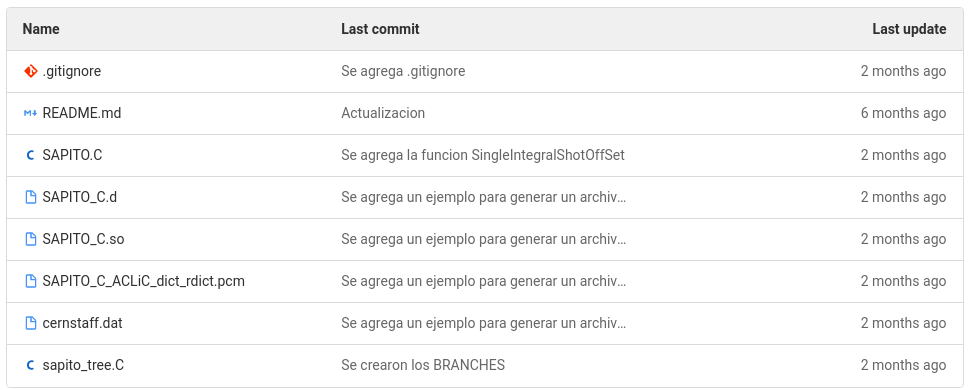
\includegraphics[width=1\textwidth]{img/Screenshot from 2021-11-22 17-40-51.png}
    \centering
    \caption{Estructura del proyecto sapito-program en GitLab.}
\end{figure}



el cual a la fecha de la presente entrada, tiene 12 commits siendo el último de SHA \verb|4582213d| con nombre de commit ``Se crearon los BRANCHES'', donde se modifica el archivo de nombre \verb|sapito_tree.C| el cual es un programa que genera un archivo \verb|.root| llamado \verb|sapito_shot.root|. Este es un archivo con estructura tipo TTree, que representa un conjunto de datos en forma de columnas (que en la jerga de \textit{root} se le llama también \textit{tree}), donde cualquier tipo de variable de \verb|C++| puede ser almacenado en sus columnas. Este \textit{tree} de nombre \verb|T|, posee 16 \textit{branches} (ramas o columnas). Las cuales son mostradas a continuación como extracto del código.


\begin{lstlisting}[language=C++]
/*ANALYSIS PARAMETERS*/
  Int_t shot;
  Int_t ch;
  double_t integral;
  double_t neutrons;
  Int_t saturated;
  std::string step;
  
/*PLASMA FOCUS CONDITIONS*/
  std::string gas;
  double_t voltage;
  double_t pressure;
  
/*DETECTOR PARAMETERS*/  

  std::string orientation;
  std::string moderator;
  Int_t angle;
  Int_t shadowC;
  Int_t test;
  double_t distance;
  double_t detector;

/*EXPERIMENTAL DATE*/
  Int_t day;
  Int_t hour;
  Int_t min;


  TFile *myfile = new TFile("sapito_shot.root","CREATE"); //Creamos un archivo root
  
  TTree *mytree = new TTree("T","SHOTS ANALYSIS"); //Creamos un tree de nombre "T"
  
  mytree->Branch("Shot",&shot,"shot/I");
  mytree->Branch("Channel",&ch,"Channel/I");
  mytree->Branch("Integral",&integral,"Integral/I");
  mytree->Branch("Neutrons",&neutrons,"Neutrons/I");
  mytree->Branch("Saturated",&saturated,"Saturated/I");
  mytree->Branch("Step",&step,"Step/I");
 //mytree->Branch("Gas",gas,"Gas/C");
  mytree->Branch("Voltage",&voltage,"Voltage/I");
  mytree->Branch("Pressure",&pressure,"Pressure/I");
 // mytree->Branch("Orientation",orientation,"Orientation/C");
  //mytree->Branch("Moderator",moderator,"Moderator/C");
  mytree->Branch("Angle",&angle,"Angle/I");
  mytree->Branch("Shadow_Cone",&shadowC,"Shadow Cone/I");
  mytree->Branch("Test",&test,"Test/I");
  mytree->Branch("Distance",&distance,"Distance/I");
  mytree->Branch("Detector",&detector,"Detector/I");
  mytree->Branch("Day",&day,"Day/I");
  mytree->Branch("Hour",&hour,"Hour/I");
  mytree->Branch("Min",&min,"Minute/I");
  \end{lstlisting}
  
 
Posteriormente (hoy) se hizo una actualización al programa \verb|SAPITO.C| agregándole dos nuevas funciones (actualización que había quedado atrasada) de nombres:

\begin{itemize}
\item[•]  \verb|double_t SingleIntegralShotOffSet_O(TString shot, int ch, int binx1, int binx2)|
\item[•] \verb|void IntegralShotOutput(TString shot)|
\end{itemize}
Donde la primera retorna la integral de un canal de un disparo con el offset ajustado usando FitAOSmovilSp, en un intervalo
determinado. La segunda retorna el archivo \verb|integral_neutrones_shot.txt| donde en tres columnas se muestra el disparo, canal e integral correspondiente al canal. Las integrales se calculan con la función descrita anteriormente.

También se hizo una actualización del programa \verb|sapito_tree.C|, resolviendo unos errores de tipo y agregándole una nueva rama tipo \verb|Int_t| y de nombre \verb|step| la cual entrega información correspondiente al fenómeno de pulso invertido.

Por último se actualizó el archivo \verb|.gitignore| para que excluya el archivo \verb|integral_neutrones_shot.txt| al hacer \verb|git push|.

De esta manera, el proyecto en GitLab queda de la siguiente manera:

\begin{figure}[H]
    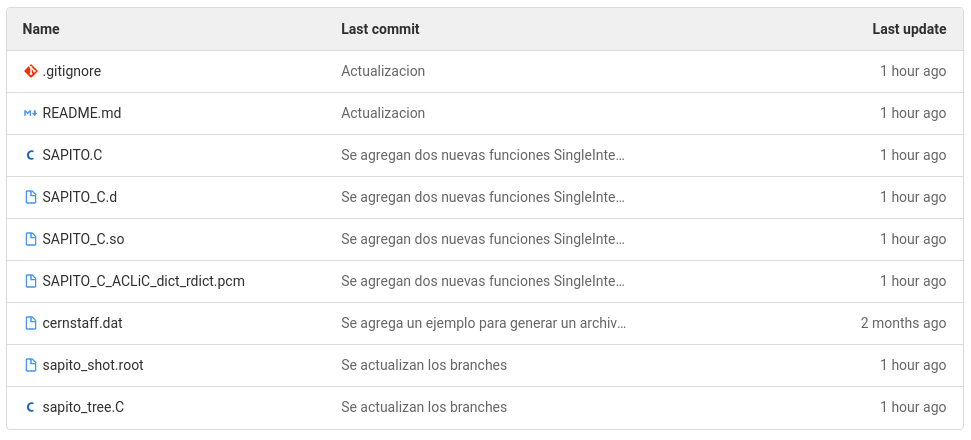
\includegraphics[width=1\textwidth]{img/Screenshot from 2021-11-22 21-17-32.png}
    \centering
    \caption{Estructura del proyecto sapito-program en GitLab.}
    \label{fig:PCG_ECG}
\end{figure}

\begin{tipt}
Para hacer un \verb|git push| a archivos modificados con distintos \verb|commits|, hacemos lo siguiente:

\begin{itemize}
\item[•]Nos movemos al directorio del programa, donde ya se encuentra creado el directorio oculto \verb|.git|
\item[•] \verb|git status| \quad Verificamos el estado del branch 
\item[•] \verb|git add programa.C| \quad Agregamos el archivo a actualizar 
\item[•] \verb|git status| \quad  Verificamos el estado del branch, debería aparecer el archivo agregado, listo para hacer el commit
\item[•] \verb|git commit -m "comentario" programa.C| \quad Hacemos el commit y agregamos un comentario 
\item[•] \verb|git push| \quad Subimos la actualización al servidor de GitLab 
\item[•] Repetir lo mismo para cada archivo a actualizar.
\end{itemize}
\end{tipt}

A partir del proyecto anterior, y en específico del programa \verb|SAPITO.C| se creó una clase que agrupa todas las funciones de este programa, permitiendo así una mejor y simple implementación de códigos futuros. El proyecto de la clase tiene por nombre en GitLab \verb|Class ANPulses| y cuyo repositorio es:

\begin{itemize}
\item \url{https://gitlab.com/flopus/class-anpulses}
\end{itemize}

La clase tiene por nombre \verb|ANPulses| y consta de los archivos \verb|ANPulses.h| donde se declaran las clases, y del archivo \verb|ANPulses.cc| donde se implementan. La última actualización en GitLab fue el 2021-11-09 donde se agregaron todas la mayoría de las funciones de \verb|SAPITO.C|, además la clase se puede probar ejecutando el programa \verb|test.C|.

\begin{tip}
Para ejecutar el código, se necesita generar antes el diccionario de la clase \verb|ANPulses|, para esto hacemos lo sisguiente:

\begin{itemize}
\item \verb|root -l| \quad Ingresamos a root
\item \verb|.L ANPulses.cc++| \quad Compilamos la macro con ACLiC, con el primer \verb|+| generamos la biblioteca compartida (shared library) de la clase \verb|ANPulses|, que recibe el nombre \verb|ANPulses_cc.so| haciendo que los símbolos del programa ( \verb|ANPulses.cc|) estén disponibles para ser cargados desde el \verb|.so| en la memoria y puedan así ser utilizados desde dentro del interprete por otros programas, además el comando \verb|+| también reconstruye (rebuild) la librería solo si el script o algunos de los archivos que incluye son más nuevos que la biblioteca. Para asegurarnos que la biblioteca partida sea reconstruida usamos el \verb|++|, generando el archivo \verb|ANPulses_cc.d|. También se genera un pre-compiled module (\verb|.pcm|) de nombre \verb|ANPulses_cc_ACLiC_dict_rdict.pcm|.
\item \verb|.L test.C++| \quad Compilamos la macro con ACLiC donde haremos la prueba de la clase (se generarán los mismos archivos explicados anteriormente).
\item \verb|test()| \quad Ejecutamos la función \verb|test()| que está definida dentro de \verb|test.C|
\end{itemize}
\end{tip} 

Par entender mejor lo anterior, de la guía de usuario de root \url{https://root.cern.ch/root/htmldoc/guides/users-guide/Cling.html#aclic-compiling-scripts-into-libraries} tenemos lo siguiente :

\begin{displayquote}
\section*{9.4 ACLiC: Compiling Scripts Into Libraries}
Instead of having Cling interpret your script there is a way to have your scripts compiled, linked and dynamically loaded using the C++ compiler and linker. The advantage of this is that your scripts will run with the speed of compiled C++ and that you can use language constructs that are not fully supported by Cling. On the other hand, you cannot use any Cling shortcuts (see “C++ Extensions To Ease Scripting” above) and for small scripts, the overhead of the compile/link cycle might be larger than just executing the script in the interpreter.

\textbf{ACLiC will build a \emph{dictionary} and a \emph{shared library} from your C++ script}, using the compiler and the compiler options that were used to compile the ROOT executable. You do not have to write a Makefile remembering the correct compiler options, and you do not have to exit ROOT.

\subsection*{9.4.1 Usage}
Before you can compile your interpreted script you need to add include statements for the classes used in the script. Once you did that, you can build and load a shared library containing your script. To load it use the command .L and append the file name with a +.

\verb|root[] .L MyScript.C+|

\textbf{The} \verb|+| \textbf{option generates the \emph{shared library}} and names it by taking the name of the file “filename” but replacing the dot before the extension by an underscore and by adding the shared library extension for the current platform. For example on most platforms, \verb|hsimple.cxx| \textbf{will generate} \verb|hsimple_cxx.so|.

\textbf{The} \verb|+|\textbf{ command \emph{rebuild} the library only if the script or any of the files it includes are newer than the library}. When checking the timestamp, ACLiC generates a dependency file which name is the same as the library name, just replacing the ‘so’ extension by the extension ‘d’. For example on most platforms, \verb|hsimple.cxx| \textbf{will generate} \verb|hsimple_cxx.d|.

\textbf{To ensure that the shared library is rebuilt you can use the} \verb|++| \textbf{syntax}:

\verb|root[] .L MyScript.C++|

To build, load, and execute the function with the same name as the file you can use the .x command. This is the same as executing a named script; you can also provide parameters. The only difference is you need to append a \verb|+| or a \verb|++|.

\verb|root[] .x MyScript.C+(4000)|\\
Creating shared library \verb|/home/./MyScript_C.so|

You \textbf{can select} whether \textbf{the script in compiled} with \emph{\textbf{debug symbol}} or with \emph{\textbf{optimization}} by appending the letter \textbf{‘g’} or \textbf{‘O’} after the ‘\verb|+|’ or ‘\verb|++|’. Without the specification, the script is compiled with the same level of debugging symbol and optimization as the currently running ROOT executable. For example:

\verb|root[] .L MyScript.C++g|

will compile MyScript.C with debug symbols; usually this means giving the \verb|-g| option to compiler.

\verb|root[] .L MyScript.C++O|

will compile MyScript.C with optimizations; usually this means giving the \verb|-O| option to compiler. The syntax:

\verb|root[] .L MyScript.C++|

is using the default optimization level.

\end{displayquote}

\section{Entrada del 2021-11-23}
\label{2021-11-23}

Se hizo una actualización de la clase \verb|ANPulses| agregando varias funciones nuevas para implementar una nueva función importante, llamada \verb|Test_Unfolding()| la cuál devuelve en pantalla el número de neutrones simulados o calculados, a partir de un flujo inventado y eficiencias absolutas, pero ahora noté que en realidad le pasamos a la función las eficiencias intrínsecas (correspondientes a seis matrices-detectores) como archivos \verb|.root| resultantes de simulaciones en Geant4. Por lo tanto, en la función \verb|Test_Unfolding()| necesitamos implementar un cálculo previo al cálculo de los neutrones simulados.

Por ahora, en GitLab actualizaremos la clase a este estado, donde en \verb|test.C| le agregamos la función \verb|Test_Unfolding()| para probarla. Además agregamos el programa de prueba \verb|flujos_inventados.C| en el cual generamos un canvas de 4x4 para visualizar los distintos flujos inventados variando los parámetros \verb|par1|  y \verb|par2|, que corresponden al centroide y ancho de una distribución gaussiana.

Se procedió a actualizar el repositorio origin/main desde el repositorio local main del pclin5 que se encuentra en el lab LIN de la cchen, quedando el repositorio en GitLab como:


\begin{figure}[H]
    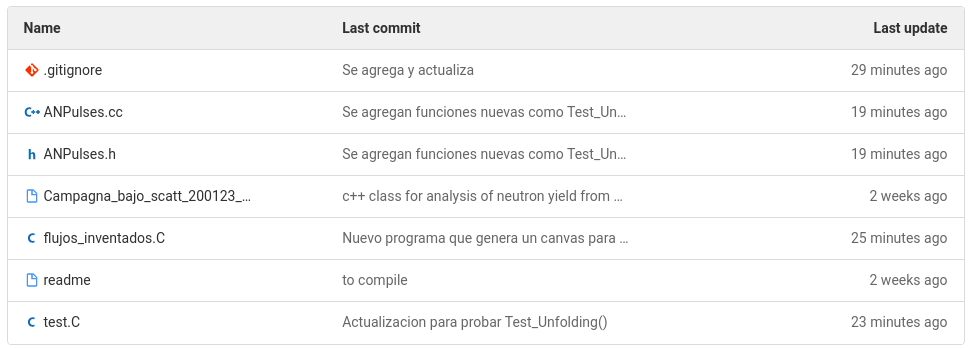
\includegraphics[width=1\textwidth]{img/Screenshot from 2021-11-23 15-58-25.png}
    \centering
    \caption{Estructura del proyecto class-anpulses  en GitLab.}
\end{figure}

Al tratar de hacer un \verb|git pull| desde mi repositorio local en mi thinkpad-t430, arrojó el siguiente error en la terminal:


\begin{lstlisting}
hint: Pulling without specifying how to reconcile divergent branches is
hint: discouraged. You can squelch this message by running one of the following
hint: commands sometime before your next pull:
hint: 
hint:   git config pull.rebase false  # merge (the default strategy)
hint:   git config pull.rebase true   # rebase
hint:   git config pull.ff only       # fast-forward only
hint: 
hint: You can replace "git config" with "git config --global" to set a default
hint: preference for all repositories. You can also pass --rebase, --no-rebase,
hint: or --ff-only on the command line to override the configured default per
hint: invocation.
\end{lstlisting}

\begin{tipt}
Cuya solución fue la siguiente (vista en \url{https://stackoverflow.com/a/32877954}):\\

\verb|git reset --hard|\\

\verb|git pull|
\end{tipt}

\subsection{Pruebas con la función Test Unfolding() }

En la clase \verb|ANPulses| tenemos implementada la función \verb|Test_Unfolding(double_t par1, double_t par2)| que toma seis eficiencias intrínsecas simuladas:

\begin{itemize}
\item[•]\verb|Efi_219_M_V4.root|
\item[•]\verb|Efi_284_M_V4.root|
\item[•]\verb|Efi_C12_V4.root|
\item[•]\verb|Efi_C15_V4.root|
\item[•]\verb|Efi_C20_V4.root|
\item[•]\verb|Efi_919_M_V4.root|
\end{itemize}

correspondientes a distintas matrices moderadoras. \\

Luego haciendo la siguiente operación:



\begin{align}\label{neutrones_calculados}
\tilde{N}_{i}^{(s)} = \sum_{j=1}^{G} \varepsilon_{ij}^{abs} \Upsilon_{j}^{(s)}
\end{align}

donde $\tilde{N}_{i}^{(s)}$ corresponde al número de neutrones calculados para cada paso $s$ de la deconvolución asociado al detector $i$, $\varepsilon_{ij}^{abs}$ es la eficiencia absoluta del detector $i$ para el grupo de energía $j$, $G$ es el número de grupos de energías y $ \Upsilon_{j}^{(s)}$ es el Yield simulado (inventado) para el grupo de energía $j$ en el paso $s$.

Dentro de la implementación de la función \verb|Test_Unfolding(double_t par1, double_t par2)| las definiciones anteriores se asocian a objetos de \verb|c++| tal y como lo muestra la siguiente tabla:

\begin{table}[H]
\centering
\begin{tabular}{|c|c|c|c|}
\hline
\textbf{Definición} & \textbf{Notación} & \verb|c++| \textbf{Type} & \textbf{Objeto} \\
\hline
Eficiencia intrínseca (simulada) & $\varepsilon_{ij}^{abs}$ & \verb|vector< vector<Double_t>>| &\verb|R[i][j]| \\
\hline
Yield inventado & $\Upsilon_{j}^{(s)}$ & \verb|vector<double>| &\verb|Phi_inv[j]| \\
\hline
\begin{tabular}{@{}c@{}} Número de neutrones calculados \\ o simulados \end{tabular}   & $\tilde{N}_{i}^{(s)}$ &\verb|vector<double>| & \verb|N[i]| \\
\hline
\end{tabular}
\caption{Implementación de los elementos de la ecuación \ref{neutrones_calculados} mediante objetos de c++.}
\end{table}


Donde la parte del código donde se implementa esto corresponde a:

\begin{lstlisting}[language=C++]
/*Numero de neutrones calculados: convolucionados, simulados o inventados por detector (i): N_i = sum efi_abs_ij*flux_j */
	for (int i = 0; i < ndet; i++)
	{
		double sum=0;
		for (int j = 0; j < binnum; j++){
			sum += R[i][j]*Phi_inv[j];
		}
		N[i] = sum;
		sum = 0;
	}
\end{lstlisting}

De esta manera, la salida del programa $\verb|test()|$ para \verb|Test_Unfolding(2.5, 0.2)| es:

\emph{\textbf{Neutrones calculados}} para cada sistema matriz-detector (son seis):


\begin{lstlisting}[language=bash]
0.213356
0.000185711
0.219751
0.231793
0.187708
0.0808738
\end{lstlisting}

\emph{\textbf{Flujo inventado:}}


\begin{figure}[H]
\centering
    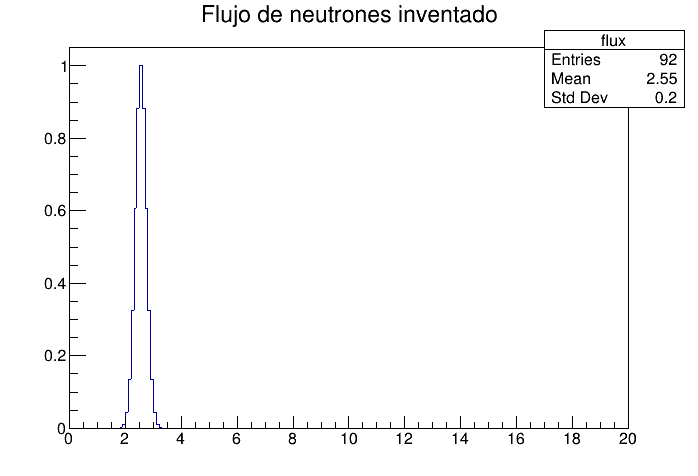
\includegraphics[width=1\textwidth]{img/c1.png}
    \caption{Flujo de neutrones inventado con valor de centroide 2.5 y sigma 0.2.}
\end{figure}



\section{Entrada del 2021-11-24}
\label{2021-11-24}

Como notamos anteriormente, en la entrada (\ref{2021-11-23}), en la función \verb|Test_Unfolding()| necesitamos implementar el cálculo de la eficiencia absoluta, el cuál lo realizamos de la siguiente manera:


\begin{lstlisting}[language=C++]
	Double_t SolAng_Dec1 = SolidAngle(200, 10, 42.5);		// G219_M
	Double_t SolAng_Dec2 = SolidAngle(200, 20, 42.5);		// G284_M
	Double_t SolAng_Dec3 = SolidAngle(200, 12, 42.5);		// C12
	Double_t SolAng_Dec4 = SolidAngle(200, 15, 42.5);		// C15
	Double_t SolAng_Dec5 = SolidAngle(200, 20, 42.5);		// C20
	Double_t SolAng_Dec6 = SolidAngle(200, 15, 42.5);		// G919_M

	/*Cargamos las eficiencias absolutas(?) al vector de vectores R*/
	R.push_back(  Readfile("/home/flopez/Data/FuncionesRespuestaByron2020/Efi_219_M_V4.root", "E219_M",SolAng_Dec1/(4*M_PI),cutbinlow, cutbinup)) ;
	R.push_back(  Readfile("/home/flopez/Data/FuncionesRespuestaByron2020/Efi_284_M_V4.root","E284_M", SolAng_Dec2/(4*M_PI), cutbinlow, cutbinup) );
	R.push_back(  Readfile("/home/flopez/Data/FuncionesRespuestaByron2020/Efi_C12_V4.root","EC12", SolAng_Dec3/(4*M_PI), cutbinlow, cutbinup) );
	R.push_back(  Readfile("/home/flopez/Data/FuncionesRespuestaByron2020/Efi_C15_V4.root","EC15",SolAng_Dec4/(4*M_PI), cutbinlow, cutbinup) );
	R.push_back(  Readfile("/home/flopez/Data/FuncionesRespuestaByron2020/Efi_C20_V4.root","EC20",SolAng_Dec5/(4*M_PI), cutbinlow, cutbinup) );
	R.push_back(  Readfile("/home/flopez/Data/FuncionesRespuestaByron2020/Efi_919_M_V4.root","E919_M",SolAng_Dec6/(4*M_PI),cutbinlow, cutbinup) );
\end{lstlisting}

Obteniendo un número de neutrones calculados por el sistema matriz-detector igual a (para un centroide de 2.5 y ancho 0.2):

\begin{lstlisting}[language=bash]
0.000179329
3.11895e-07
0.000221615
0.000292125
0.000315249
0.000101924
\end{lstlisting}

\begin{tip}
Una cantidad considerablemente menor de neutrones, en comparación con el caso anterior. Entonces, necesitamos un flujo de mayor intensidad, es decir, subir el yield total (la integral). Para esto le ponemos un factor $A$ a la distribución gaussiana, es decir $A\cdot \exp$, y lo vamos variando.
\end{tip}

Notemos que la integral del flujo inventado antes de aplicar el factor $A$ corresponde a 5.013, tal y como se ve en la Fig. \ref{flujo_inventado_sin_factor}:

\begin{figure}[H]
\centering
    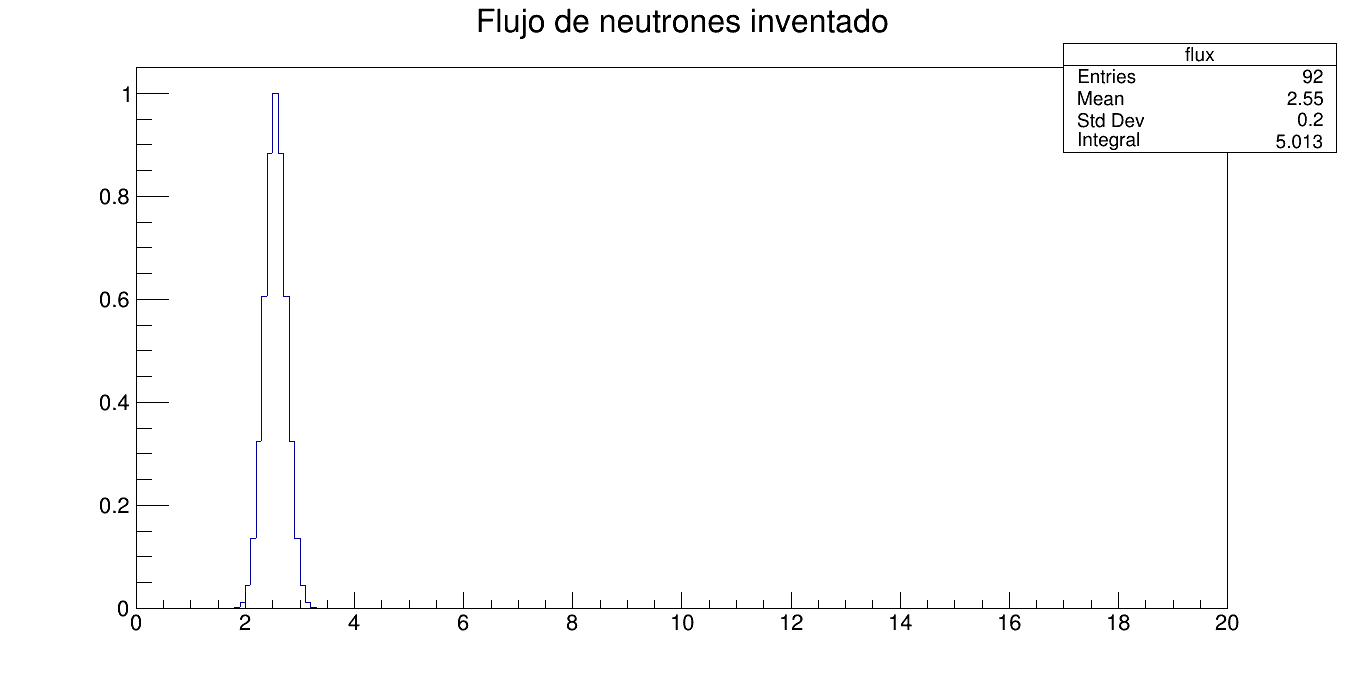
\includegraphics[width=1\textwidth]{img/c1_integral_sin_factor.png}
    \caption{Integral del flujo de neutrones inventado con valor de centroide 2.5 y sigma 0.2.} \label{flujo_inventado_sin_factor}
\end{figure}

Entonces, modificamos la función \verb|SeedGenerator()| de la clase \verb|ANPulses| para incorporar un factor que controle la intensidad del yield total del flujo inventado. Este factor se llamara $A$ y pasa a ser un nuevo parámetro de la función:

\begin{lstlisting}[language=C++]
...
vector<Double_t> ANPulses::SeedGenerator(double* bins, double A=1.0, int binnum, double par1, double par2)
...
double content = 0;
vector<Double_t> seed(binnum, 0);

...

	// Gauss //
	
	for (int i = 0; i < binnum; i++){
		content = 0;
		content = A*TMath::Gaus(bins[i], par1, par2);
		seed[i] = content;
	}
\end{lstlisting}

De esta manera, el la función \verb|Test_Unfolding()| definimos el factor como $A=1000.$, resultando así el número de neutrones calculados como:


\begin{lstlisting}[language=bash]
0.179329
0.000311895
0.221615
0.292125
0.315249
0.101924
\end{lstlisting}

Y la integral del flujo corresponde a 5013 (aumenta en un factor de 1000 con respecto al anterior, tal y como se esperaba):

\begin{figure}[H]
\centering
    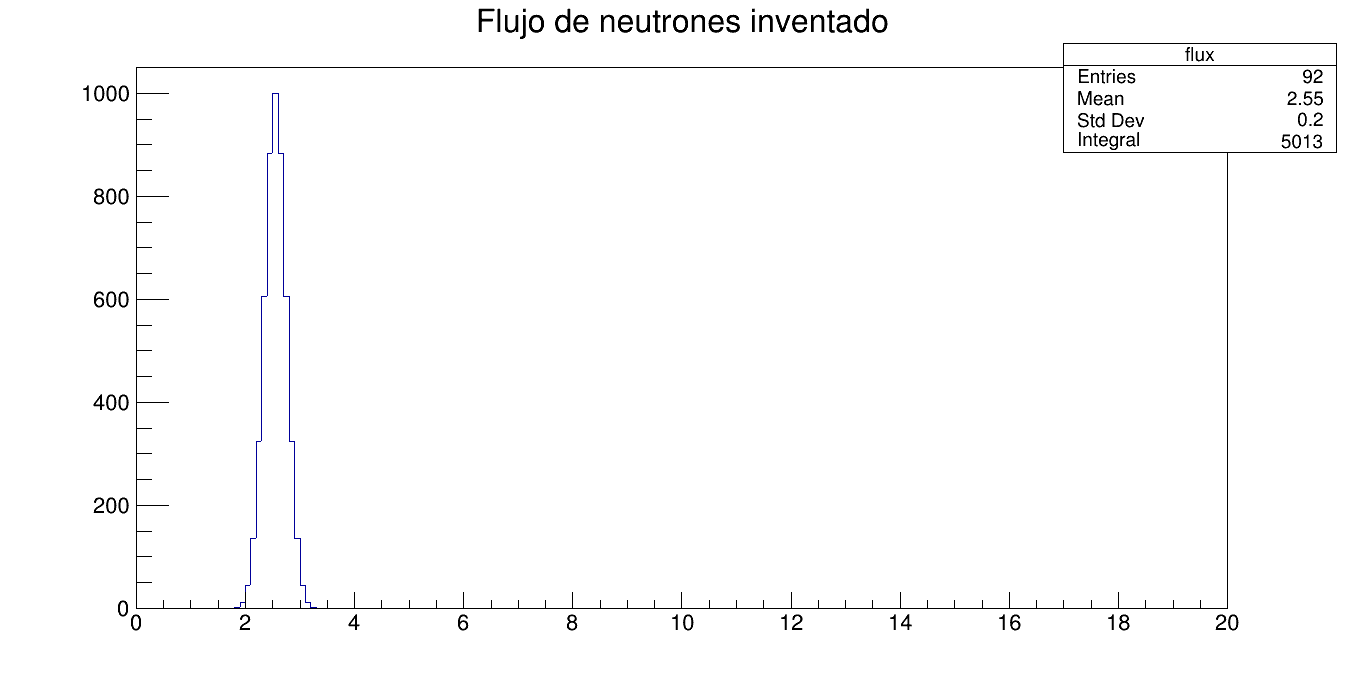
\includegraphics[width=1\textwidth]{img/c1_integral_con_factor.png}
    \caption{Integral del flujo de neutrones inventado con valor de centroide 2.5 y sigma 0.2. con factor $A=1000.$}
    \label{flujo_inventado_con_factor}
\end{figure}

Ahora haremos unas modificaciones a la función \verb|Test_Unfolding()|, de tal manera que genere un archivo como salida donde se almacenen los neutrones calculados para cada sistema matriz-detector.


\begin{lstlisting}[language=C++]
ofstream neutrones_calculados("neutrones_calculados.dat"); // archivo de salida
...
/*Generamos un archivo con los neutrones calculados*/
for (int i = 0; i < ndet; i++) 
{
	neutrones_calculados<<setw(5) << setfill(' ') << N[i] << " ";
}
neutrones_calculados.close();
...
\end{lstlisting}

Finalmente en la clase \verb|ANPulses|, implementamos la función que realiza la deconvolución de los neutrones calculados, llamada \verb|Pretty_EMsimple()|, la cuál toma varias parámetros de entrada:

\begin{lstlisting}[language=C++]
void ANPulses::Pretty_EMsimple(int shot, int steps=100, double par1=2.5, double par2=0.02, TString Type="Dif", int rebin=1, int bin_l=12)
\end{lstlisting}

Y en su implementación necesita un archivo con los neutrones calculados y uno con los errores de ellos, el cual lo llenamos de valores 1:

\begin{lstlisting}[language=C++]
...
//Le pasamos un numero de neutrones simulados o calculados del Test_Unfolding()
...
N = ReadData("neutrones_calculados.dat", shot, ndet+1); 
...
N_Err = ReadData("neutrones_calculados_err.dat", shot, ndet+1, kFALSE);
...
\end{lstlisting}

Necesita también las eficiencias intrínsecas, para que internamente se calculen las eficiencias absolutas a partir de ellas. Además, se define el flujo semilla del algoritmo, que corresponde a una distribucion gaussiana:

\begin{lstlisting}[language=C++]
...
/*Flujo semilla*/
Seed = SeedGenerator(bins, binnum, 1.0, par1, par2); 
...
\end{lstlisting}

De esta manera, en el programa \verb|test.C| generamos la instancia de la función con los siguientes parámetros:

\begin{lstlisting}[language=C++]
...
cout << "Test de deconvolucion" << endl;
pulse.Pretty_EMsimple(1, 100, 2.5, 0.2,"Dif", 1, 12);
...
\end{lstlisting}

Produciendo entonces al ejecutar \verb|test()|, la siguiente salida en la terminal de root: 

\begin{lstlisting}[language=bash]
Test de deconvolucion
Binning		V4
Steps		100
cutbinlow	1
cutbinup	1
Detectors	6

Shot number:  1
Detectors Status and Counting
Detector   1		0.179329
Detector   2		0.000311895
Detector   3		0.221615
Detector   4		0.292125
Detector   5		0.315249
Detector   6		0.101924

Neutrones Deconvolucionados
	0.150513
	0.000214608
	0.18498
	0.242506
	0.25991
	0.0822296
Diferencia porcentual
	16.0688
	31.1923
	16.5309
	23.0747
	155.003
	19.3226

Integral: 4129.57
Xi^2	: 0.438394
St Dv	: 0
Warning in <TCanvas::Constructor>: Deleting canvas with same name: c1
 FCN=45.2331 FROM MIGRAD    STATUS=CONVERGED      64 CALLS          65 TOTAL
                     EDM=1.61303e-08    STRATEGY= 1      ERROR MATRIX ACCURATE 
  EXT PARAMETER                                   STEP         FIRST   
  NO.   NAME      VALUE            ERROR          SIZE      DERIVATIVE 
   1  Constant     7.75833e+02   1.47213e+01   4.03053e-02   5.87828e-06
   2  Mean         2.49841e+00   3.29275e-03   1.09120e-05  -3.56939e-02
   3  Sigma        2.10022e-01   2.25391e-03   9.70061e-06  -2.09220e-02
Error in <TPad::TPad>: illegal height: -0.420000
Info in <TCanvas::Print>: file EMsimple_Data_S1.png has been created
Info in <TCanvas::SaveAs>: ROOT file EMsimple_Data_S1.root has been created
\end{lstlisting}

Además genera un gráfico con la comparación de neutrones calculados y deconvolucionados:

\begin{figure}[H]
\centering
    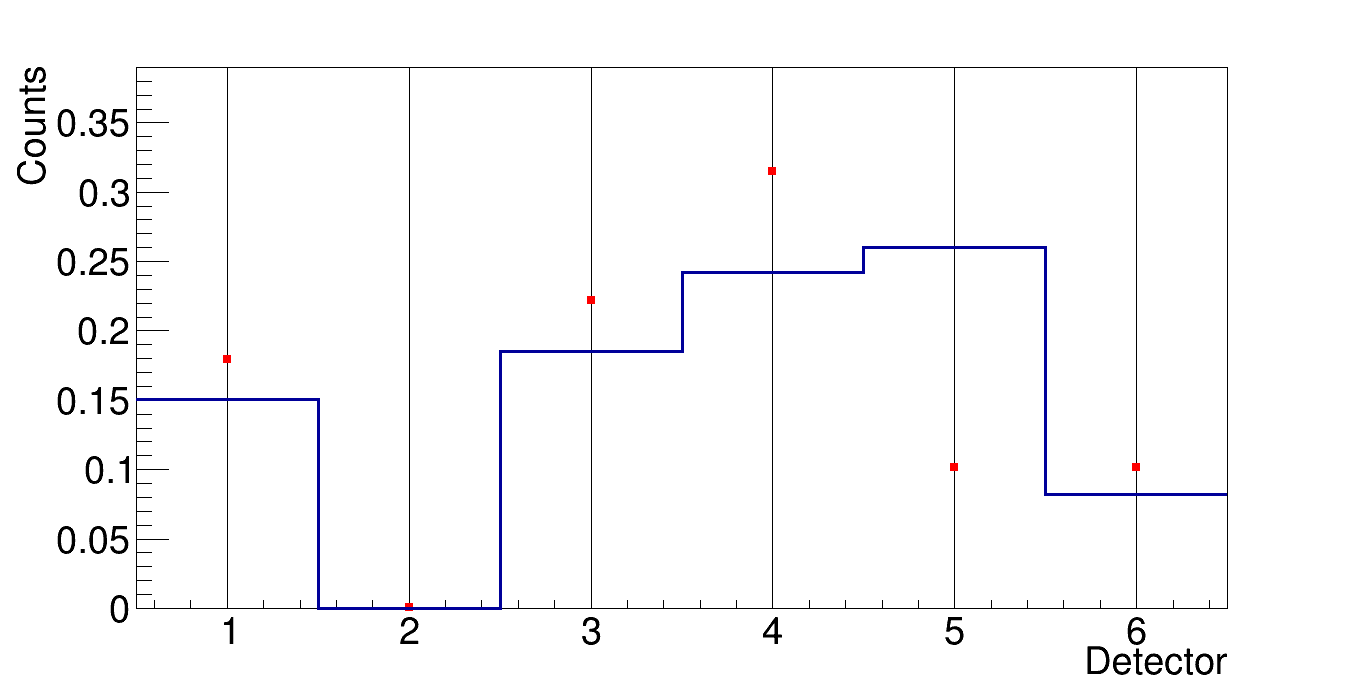
\includegraphics[width=1\textwidth]{img/EMsimple_Data_S1_01.png}
    \caption{Comparación entre neutrones calculados y deconvolucionados.}
    \label{comp_neutrones_cal_deconv_01}
\end{figure}


Al revisar la diferencias relativas porcentuales entre los neutrones deconvolucionados y calculados, note que las diferencias desde el Detector 4 al 5 son incorrectas.


\begin{table}[H]
\centering
\begin{tabular}{|c|c|c|c|c|}
\hline
\textbf{Detector} & \begin{tabular}{@{}c@{}} \textbf{Neutrones} \\ \textbf{calculados} \end{tabular}  &  \begin{tabular}{@{}c@{}}\textbf{Neutrones} \\ \textbf{deconvolucionados} \end{tabular}  & \begin{tabular}{@{}c@{}} \textbf{Dif relativa \% } \\ \textbf{código} \end{tabular} & \begin{tabular}{@{}c@{}} \textbf{Dif relativa \% }   \\ \textbf{correcta} \end{tabular} \\ 
\hline
Detector 1 & 0.179329 & 0.150513 & 16.0688 &16.06879  \\
Detector 2 & 0.000311895 & 0.000214608 & 31.1923 &31.192228  \\
Detector 3 & 0.221615 & 0.18498 & 16.5309 &16.530921  \\
Detector 4 & 0.292125 & 0.242506 & 23.0747 & 16.985537 \\
Detector 5 & 0.315249 & 0.25991 & 155.003 &17.55406  \\
Detector 6 & 0.101924 & 0.0822296 & 19.3226 &19.322633  \\
\hline
\end{tabular}
\caption{Comparación de neutrones calculados y deconvolucionados mediante la dif rel \%.}
\end{table}

Notemos de la fig (\ref{comp_neutrones_cal_deconv_01}) que los puntos de los neutrones calculados del 4 al 5 están incorrectamente graficados.
	
El error anterior, venía por las siguientes líneas de código en la función  \verb|Pretty_EMsimple()|, las cuales eliminaban la entrada 4 del vector de neutrones calculados N:

\begin{lstlisting}[language=bash]
N.erase(N.begin()+3);
N_Err.erase(N_Err.begin()+3);
\end{lstlisting}

Al comentar estas líneas, pasa algo curioso, y es que el número de neutrones deconvolucionados es el mismo que el número de neutrones calculados:

\begin{lstlisting}[language=bash]
Test de deconvolucion
Binning		V4
Steps		100
cutbinlow	1
cutbinup	1
Detectors	6

Shot number:  1
Detectors Status and Counting
Detector   1		0.179329
Detector   2		0.000311895
Detector   3		0.221615
Detector   4		0.292125
Detector   5		0.315249
Detector   6		0.101924

Neutrones calculados	
v = { 0.179329, 0.000311895, 0.221615, 0.292125, 0.315249, 0.101924, }; 
Neutrones Deconvolucionados
	0.179329
	0.000311895
	0.221615
	0.292125
	0.315249
	0.101924
Diferencia porcentual
	5.34767e-05
	9.77985e-05
	8.45083e-05
	3.49242e-05
	3.73356e-05
	6.25612e-05

Integral: 5013.25
Xi^2	: 3.81291e-13
St Dv	: 0
Warning in <TCanvas::Constructor>: Deleting canvas with same name: c1
 FCN=1.07128e-10 FROM MIGRAD    STATUS=CONVERGED      37 CALLS          38 TOTAL
                     EDM=1.11912e-13    STRATEGY= 1      ERROR MATRIX ACCURATE 
  EXT PARAMETER                                   STEP         FIRST   
  NO.   NAME      VALUE            ERROR          SIZE      DERIVATIVE 
   1  Constant     1.00000e+03   1.72980e+01   3.00000e-02  -1.93530e-08
   2  Mean         2.55000e+00   2.82469e-03   7.65000e-05   9.99301e-09
   3  Sigma        2.00000e-01   1.99740e-03   1.72186e-06  -1.74058e-04
\end{lstlisting}


\begin{figure}[H]
\centering
    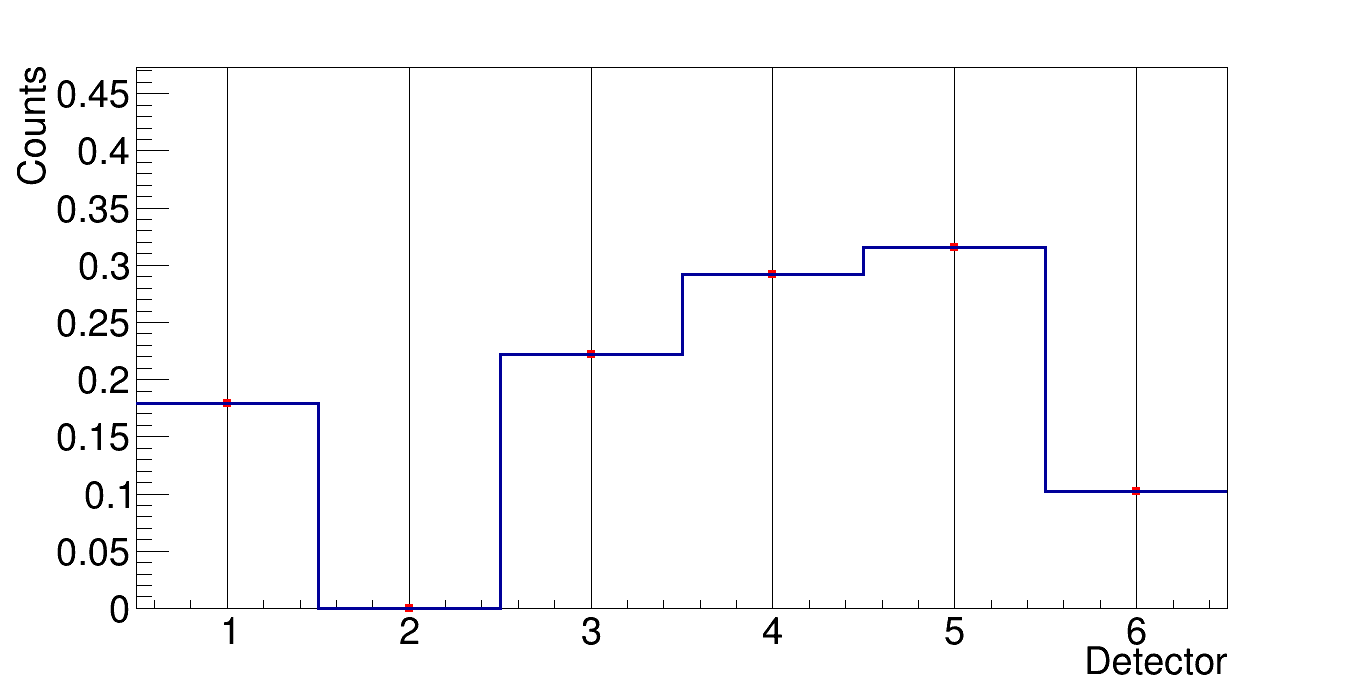
\includegraphics[width=1\textwidth]{img/EMsimple_Data_S1_02.png}
    \caption{Comparación entre neutrones calculados y deconvolucionados.}
    \label{comp_neutrones_cal_deconv_02}
\end{figure}

\begin{tipt}
Después de dar muchas vueltas a la situación, me di cuenta que estábamos usando como flujo semilla del algoritmo de deconvolución la misma distribución gaussiana que usamos como flujo inventado para calcular los neutrones calculados. Por lo que era esperable que obtuvieramos el mismo número de neutrones deconvolucionados y calculados, ya que \textbf{queremos que el algoritmo sea capaz de hacer eso} pero cuándo después le pasemos \emph{\textbf{neutrones medidos}}.
\end{tipt}

\section{Entrada del 2021-11-25}
\label{2021-11-25}

\hightodo{2021-11-25: Hacer pruebas con neutrones calculados a partir de flujos inventados no gaussianos, usando como flujo semilla de la deconvolución una distribución gaussiana.}

Llenar con la actualización del código.

Queremos encontrar un criterio de stop del $\chi^2$ reducido, donde la definición de este último corresponde al $\chi^2$ divido por el número de grados de libertad ($ndl$) del problema a tratar:

\begin{align}
\chi_{red}^2 = \frac{\chi^2}{ndl}
\end{align}

 en nuestro caso, corresponde al bineado de las eficiencias intrínsecas: 92 (\verb|binx|). Las eficiencias al pasar a objetos de $\verb|c++|$ se define como un vector. Entonces, si revisamos el siguiente código:

\begin{lstlisting}[language=C++]
R.push_back(  Readfile("/home/flopez/Data/FuncionesRespuestaByron2020/Efi_219_M_V4.root", "E219_M",SolAng_Dec1/(4*M_PI),cutbinlow, cutbinup)) ;
\end{lstlisting}

La función \verb|Readfile()| tal y como está implementado en la clase \verb|ANPulses|, retorna un vector de largo 92, que corresponde al bineado de las eficiencias intrínsecas. Luego, al hacer \verb|push_back| estamos llenando el vector $\verb|R|$ con vectores como entrada, en específico, 6 vectores, correspondientes a las eficiencias absolutas de cada sistema de detección, es decir, \verb|R| corresponde a una matriz de 6$\times$92. Este vector de vectores es el que será usado para realizar la deconvolución.

El criterio de stop lo establecemos al ver las diferencias entre flujos, para esto denotamos primero los flujos a considerar:


\begin{table}[H]
\centering
\begin{tabular}{|c|c|}
\hline
\textbf{Flujos} & \textbf{Definición}  \\ 
\hline
$\Phi_j^{inv}$ & Valor de flujo inventado para la región j de energía \\
$\Phi_j^{(s)}$ & Valor de flujo correspondiente a cada paso $s$ de la deconvolución en la región $j$ de energía  \\
$\Phi_j^{(seed)}$& Valor del flujo semilla en la región $j$ de energía  \\
\hline
\end{tabular}
\caption{Flujos a considerar en el criterio de stop $\chi^2$}
\end{table}


Entonces, definiremos $\chi^2$ como 

\begin{align}
\chi^2 = \sum_{j=1}^{M=92}\left( \frac{\Phi_j^{inv} -\Phi_j^{(s)}}{(\Phi_j^{inv}/100)} \right)^2
\end{align}

deberíamos entonces cortar en $\chi^2 \approx N$, con $N$ número de detectores.

\section{Entrada del 2021-11-29}
\label{2021-11-29}

A continuación mostraremos el algoritmo a implementar a partir de la función \verb|EM_Pretty_EMsimple()|


\begin{algorithm}[H]\label{em1}
\SetArgSty{textnormal}  %para evitar las líneas horizantes en los comandos de flujo
\KwIn{ $\vec{n}$ neutrones calculados, $\Phi^{(0)}$ flujo semilla, $R$ matriz de eficiencias absolutas (función respuesta)}
\KwOut{$\Phi^{(s)*}$ flujo de salida que satisface $\chi^2 < N$ (número de detectores)}
\While{$\chi^2>N$}{
\For{$s = 0$ \KwTo $Steps$}{
Algoritmo EM \; 
$(\Phi^{s})$ Flux = FluxNext \;
$\chi^2=\displaystyle\sum_{i=1}^{N}\frac{\left(\displaystyle\sum_{j=1}^{M}R_{ij}\Phi_j^{s}- n_i \right)^2}{\Delta n_i^2}$\;
}
}
\caption{EM1\label{EM1}}
\end{algorithm}

A continuación calculamos:

\begin{algorithm}[H]\label{em2}
\SetArgSty{textnormal} %para evitar las líneas horizantes en los comandos de flujo
%\Fn(\tcc*[h]{algorithm as a recursive function}){\FRecurs{some args}}
\KwIn{$\Phi^{(s)*}$ flujo de salida que satisface $\chi^2 < N$ (número de detectores), $\Phi^{(inv)}$ flujo inventado}
\KwOut{$\chi_c^2$}
\Return{$\chi_c^2=\displaystyle\sum_{j=1}^{M}\frac{\left(\Phi_j^{s*}- \Phi_j^{inv} \right)^2}{\left(\Delta \Phi_j^{(inv)}\right)^2}$\;}
\caption{EM2\label{EM2}}
\end{algorithm}

Con los resultados de la implementación de estos algoritmos, la idea es realizar un gráfico de $\Phi^{(inv)}$ y $\Phi^{(0)}$, donde el tercer eje corresponderá al valor de $\chi_c^2$ asociado a cada par $(\Phi^{(0)},\Phi^{(inv)})$, determinando así la dependencia del flujo deconvolucionado con respecto de la semilla inicial.


\section{Entrada del 2021-12-01}
\label{2021-12-01}

Se implementó en \verb|researchdiary_config.tex| una caja de color amarillo para las preguntas a partir del paquete \verb|todonotes| (manual: \url{http://tug.ctan.org/macros/latex/contrib/todonotes/todonotes.pdf})

\verb|\newcommand{\question}[1]{\todo[inline,backgroundcolor=yellow!90!yellow!80!white]|\\
\verb|{\textbf{\userId}: #1}}|

La cuál se utiliza de la siguiente manera: \verb|\question{2021-12-01 Pregunta}| y además aparece en el índice de Todo list.


\section{Entrada del 2021-12-02}
\label{2021-12-01}

Hasta la presente fecha teníamos atrasada la actualización en GitLab de la clase \verb|ANPulses| y demás macros nuevas, por lo que realizaremos un update del repositorio. Se agregará entonces la macro \verb|neutron_sim_generator.C|, que al ser cargada en root para luego ejecutar la función \verb|neutron_sim_generator()|, se tiene que esta itera sobre los anchos (\verb|sig|) en las funciones \verb|Test_Unfolding_TH1D(2.5,sig)| y \verb|Test_Unfolding(2.5,sig)|. Las cuales, respectivamente generan un canvas con todos los flujos inventados para distintos anchos y generan diversos archivos .dat con los neutrones calculados correspondiente a cada flujo, que luego son guardados en una carpeta de nombre \verb|./neutrones_calculados|.

Las actualizaciones realizadas a la clase \verb|ANPulses|, primero tiene que ver con los nombres de los archivos de neutrones calculados:

\begin{lstlisting}[language=C++]
void ANPulses::Test_Unfolding(double_t par1, double_t par2)
{
		/*double to String with Custom Precision using ostringstream*/
	// Create an output string stream
	std::ostringstream stream_centroide;
	std::ostringstream stream_ancho;
	// Set Fixed -Point Notation
	stream_centroide << std::fixed;
	stream_ancho << std::fixed;
	// Set precision to 1 digits
	stream_centroide << std::setprecision(1);
	stream_ancho << std::setprecision(1);
	//Add double to stream
	stream_centroide << par1;
	stream_ancho << par2;
	// Get string from output string stream
	std::string centroide = stream_centroide.str();
	std::string ancho = stream_ancho.str();
	
	ofstream neutrones_calculados("./neutrones_calculados/neutrones_calculados_C"+centroide+"_S"+ancho+".dat"); // archivo de salida
...
\end{lstlisting}

También actualizamos la función \verb|SeedGenerator()|, por lo que ahora además del factor $A$ de intensidad agregado (ver entrada \ref{2021-11-24}) tiene un nuevo parámetro tipo \verb|TString| llamado $dist$ que me permite elegir el tipo de distribución: "G" para gaussian, "AG" para asymetric gaussian. Se adicionarán más a futuro.

Se agrega también la macro \verb|file_generator.C| la cual me servirá a futuro para generar el archivo .root de la campaña. 
Por último notemos que las barras de errores de las Fig. \ref{comp_neutrones_cal_deconv_01}  y \ref{comp_neutrones_cal_deconv_02} se deben a que en el archivo \verb|neutrones_calculados_err.dat| habían solo unos en cada columna. Para evitar estas barras de error, el archivo se llena de ceros.

\begin{tipt}
\textbf{Revert commits: (\url{https://stackoverflow.com/a/14281090/17548388})}
\begin{itemize}
\item[•]\textbf{IF} you have \textbf{NOT pushed} your changes to remote:
 
\verb|git reset HEAD~1|

Check if the working copy is clean by git status. After restart from git add ...

\item[•] \textbf{ELSE} you have pushed your changes to remote: 

\verb|git revert HEAD|	

This command will revert/remove the local commits/change and then you can push. Besides, deleted all files that I had ready to push. Be careful!
\end{itemize}

\end{tipt}

La actualización del repositorio en GitLab quedó como:

\begin{figure}[H]
    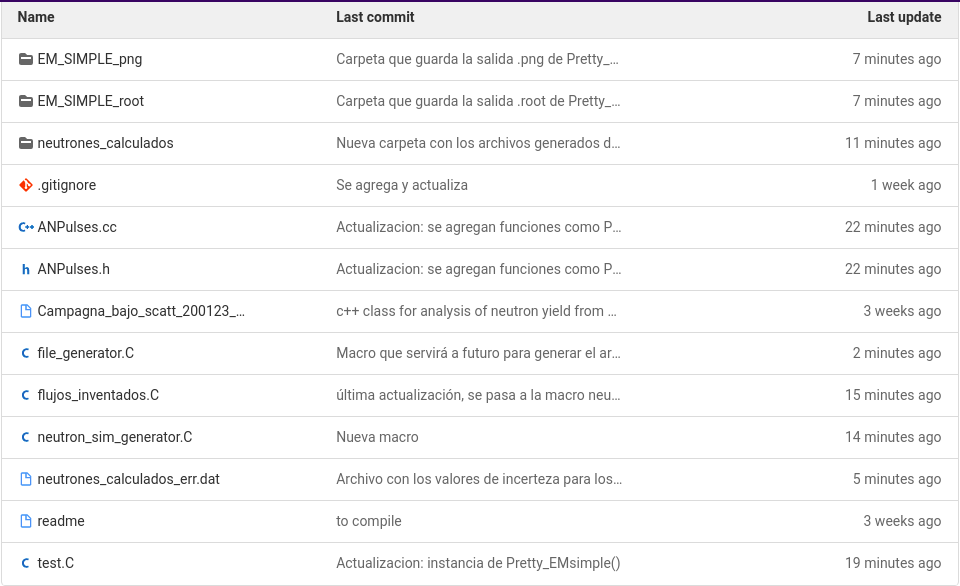
\includegraphics[width=1\textwidth]{img/Screenshot from 2021-12-02 03-42-56.png}
    \centering
    \caption{Estructura del proyecto class-anpulses  en GitLab.}
\end{figure}

Ahora implementaremos en la clase el chi-square y chi-square reducido. 

\begin{lstlisting}[language=C++]
...
double_t ANPulses::Xi_Square_red(vector<Double_t> N_i, vector<Double_t> N_rec, vector<Double_t> Err, double ndet)
{
	double_t xi=0;
	double_t partial_sum=0;
	double_t nprom=0;
	double_t variance=0;

	for (int i = 0; i < ndet; i++){ partial_sum = (N_i[i] - N_rec[i])/N_i[i]; xi += partial_sum*partial_sum; }


	/*chi-square reducido: chi-square dividido por el numero de grados de libertad (ndl) del problema, en esta caso el 
	 * numero de detectores*/
	return xi/(double (ndet));
	
}

double_t ANPulses::Xi_Square(vector<Double_t> N_i, vector<Double_t> N_rec, vector<Double_t> Err, double ndet)
{
	double_t xi=0;
	double_t partial_sum=0;
	double_t nprom=0;
	double_t variance=0;

	for (int i = 0; i < ndet; i++){ partial_sum = (N_i[i] - N_rec[i])/N_i[i]; xi += partial_sum*partial_sum; }


	return xi;
	
}
...
\end{lstlisting}

Por lo que se hizo un \verb|git push| al repositorio de commit SHA 2478ed9eae44ec7438853297012eb4e6ae155132.

Ahora necesitamos implementar los nuevos chi squares de los algoritmos EM1 y EM2. Para esto haremos los cambios en una nueva función \verb|Pretty_EMsimple_em1()|. En esta función seteamos el parámetro $A$ de intensidad de flujo de \verb|SeedGenerator()| en 1000. Luego se probaron distintos valores de $A$ para la función semilla (1,10,100,1000,10000,100000), pero no hubo cambios en el número de neutrones deconvolucionados, se mantuvo constante.

\section{Entrada del 2021-12-03}
\label{2021-12-03}


Se modificaron las funciones \verb|Test_Unfolding()| y \verb|Test_Unfolding_TH1D()| añadiendo en ambas los parámetros nuevos siguientes:

\begin{table}[H]
\centering
\begin{tabular}{|c|c|}
\hline
\textbf{Parámetro} & \textbf{Descripción}  \\ 
\hline
\verb|TString dist| & \begin{tabular}{@{}c@{}} Establece el tipo de distribución inventada  \\ a usar: \verb|"G"|: gaussian, \verb|"AG"|: asymetric gaussian  \end{tabular}  \\
\hline
\verb|double_t SIGL| & \begin{tabular}{@{}c@{}} Cuándo el parámetro \verb|dist| toma  el valor \verb|"AG"|, \\ entonces \verb|SIG_L| establece el ancho izquierdo de \\la distribución. \end{tabular} \\
\hline
\verb|double_t SIGR| & \begin{tabular}{@{}c@{}} Cuándo el parámetro \verb|dist| toma  el valor \verb|"AG"|, \\ entonces \verb|SIG_R| establece el ancho derecho de \\la distribución. \end{tabular} \\
\hline
\end{tabular}
\caption{Nuevos parámetros.}\label{new_parameters}
\end{table}

Además la función \verb|Test_Unfolding()| ahora genera los archivos de salida con los neutrones calculados con la siguiente estructura:


Se hicieron distintas actualizaciones a la clase \verb|ANPulses|. Se agregó la función  \verb|Pretty_EMsimple_em1()| la cuál servirá como función de prueba para implementar los algoritmos EM1(\ref{em1}) y EM2(\ref{em2}).  Esta función por ahora genera un canvas con los histogramas del flujo semilla,  flujo deconvolucionado y flujo inventado. Así también muestra el valor de $\chi^2$ y $\chi^2/(ndl)$ por paso $s$ de iteración del \textit{Expectation maximisation method} (EM).  Junto con esto genera un archivo de nombre \verb|xi2.txt| con los valores de $\chi^2$ y $\chi^2/(ndl)$ por paso $s$ del algoritmo. Por último acepta ahora tres parámetros más, los mismos mostrados en la tabla (\ref{new_parameters}), los cuáles en principio están pensados para usarse en el flujo semilla.   

\hightodo{2021-12-03 Implementar parámetros diferenciados para la semilla y para el flujo inventado en Pretty EMsimple em1(), tanto para el tipo de distribución como de valor de anchos. Esto para hacer la iteraciones más fáciles de programar.}

\begin{tipt}
No agregar nunca el formato \verb|\verb| en \verb|\todo| todo ya que explota el código. Si pasa esto, hay que borrar los archivos .aux .log .out y .tdo antes de volver a compilar. Para agregar ecuaciones, se debe usar el comando \verb|\protect|.
\end{tipt}

Por último la macro \verb|neutron_sim_generator.C| tiene implementada tres funciones más de tipo \verb|void|: 

\begin{table}[H]
\centering
\begin{tabular}{|c|c|}
\hline
\textbf{Función} & \textbf{Descripción}  \\ 
\hline
\verb|neutron_sim_generator_AG_R()| & \begin{tabular}{@{}c@{}} Genera 16 flujos inventados del tipo "asymetric \\ gaussian" donde el parámetro sobre el que se itera \\ corresponde al ancho de la gaussiana derecha y dejando el \\ ancho izquierdo fijo. Generando entonces 16 archivos con\\ neutrones calculados.   \end{tabular}  \\
\hline
\verb|neutron_sim_generator_AG_L()| & \begin{tabular}{@{}c@{}} Genera 16 flujos inventados del tipo "asymetric \\ gaussian" donde el parámetro sobre el que se itera \\ corresponde al ancho de la gaussiana izquierda y dejando el \\ ancho derecho fijo. Generando entonces 16 archivos con \\ neutrones calculados.   \end{tabular}  \\
\hline
\verb|neutron_sim_generator_AG_RL()| & \begin{tabular}{@{}c@{}} Genera 16 flujos inventados del tipo "asymetric\\ gaussian" donde los parámetros sobre los que se iteran\\ corresponden al ancho derecha e izquierdo de la distribución\\ gaussina, 4 iteraciones para cada ancho. Generando \\ entonces 16 archivos con neutrones calculados.  \end{tabular}  \\
\hline
\end{tabular}
\caption{Nuevos parámetros.}
\end{table}

\section{Entrada del 2021-12-06}
\label{2021-12-06}
Actualización del repositorio en GitLab con todo lo nombrado en la entrada anterior (\ref{2021-12-03}).


Quiero generar una nueva función \verb|ReadData()| que lea un archivo de texto, donde en la primera columna de este archivo se encuentre el número de disparo y seguido, los neutrones calculados correspondientes a cada detector, y por último, la información del flujo inventado: \verb|dist|, \verb|par1|, \verb|par2|, \verb|SIG_L| \verb|SIG_L| según corresponde. Algo como lo siguiente:

\begin{lstlisting}[language=bash]
...
9 0.1675 0.000212405 0.205418 0.268571 0.286972 0.089015 AG 2.5 1.0 1.3 0.5	
...
\end{lstlisting}

\hightodo{2021-12-06: Hacer pruebas variando los flujos inventados y los flujos semilla. \textbf{HECHO, ver entrada (\ref{2021-12-14})}}

\section{2021-12-07}
\label{2021-12-07}
Actualización del repositorio en GitLab, donde se crea la función:

\begin{lstlisting}[language=bash]
...
void ANPulses::Test_Unfolding_shots(int shot, double_t par1, double_t par2, TString dist, double_t SIG_L, double_t SIG_R)
...
\end{lstlisting}

la cuál genera un archivo de nombre \verb|neutrones_calculados_merge.dat| donde se guarda la información de una simulación (``shot'') tal y como se muestra en la entrada \ref{2021-12-06}). La idea de esta función es poder iterar sobre ella generando neutrones simulados correspondientes a distintos flujos inventados (gausianos y gausianos asimétricos).


Luego se agregó a la clase \verb|ANPulses| la función:

\verb|vector<Double_t> ANPulses::ReadDataShot(TString fname, int shot, int ndet=3)|

la cuál lee un archivo creado por la función anterior, donde están ordenados los disparos por filas, junto con el número de neutrones por detector y parámetros del flujo inventado con los cuáles se calculan estos neutrones. La función retorna un vector de neutrones calculados, correspondientes a un disparo determinado.  

En la macro \verb|neutron_sim_generator.C| se agrega la función \verb|void neutrones_sim_generator_merge()| la cuál itera sobre la función \verb|Test_Unfolding_shots()| para distintos valores de ancho de una distribución gaussiana. Llenando así el archivo \verb|neutrones_calculados_merge.dat|.

Flujo diferencial es el dividido por $dE$.


Método de Deconvolución: Máxima Expectación

\begin{align}
\Upsilon_b^{(s+1)} = \frac{1}{\displaystyle\sum_{r}^{ndet} \varepsilon_{rb}^{(abs)}}\displaystyle \sum_{r}^{ndet}\frac{\varepsilon_{rb}^{(abs)} \Upsilon_b^{(s)}N_r}{\displaystyle \sum_{k}^{binnum} \varepsilon_{rk}^{abs}\Upsilon_k^{(s)}}
\end{align}

donde $\Upsilon_b^{(s+1)}$ corresponde al Yield obtenido para la iteración $(s+1)$ en el grupo (bin) de energía $b$, $\varepsilon_{rb}^{(abs)}$ corresponde a la eficiencia absoluta del detector $r$ para el grupo de energía $b$, $N_r$ es el número de neutrones detectados por el detector $r$, $binnum$ corresponde al de grupo de energías y $ndet$ corresponde a la cantidad de detectores.

Algoritmo de deconvolucion EM implementado en \verb|c++|:

\begin{lstlisting}[language=c++]
for(int it=0; it<steps*1.5; it++){ /*Al multiplicar: steps*1.5, hacemos 1.5 veces mas pasos en la iteracion*/
	FluxNext = Flux;
		
	for(Int_t b=0; b<binnum; b++)
	 {
			Sum_R=0.;
			for(Int_t r=0; r<ndet; r++)	Sum_R += (R[r][b]); /*<@$\displaystyle\sum_{r}^{ndet} \epsilon_{rb}^{(abs)}$@>*/
			
				Sum_N_R_Flux=0.;
				
				for(Int_t r=0; r<ndet; r++)
					{
						Sum_R_Flux=0.;
						
							for(Int_t k=0; k<binnum; k++)
								{
								  Sum_R_Flux += (R[r][k] * Flux[k] * dE[k]); // *dE  <@$\displaystyle \sum_{k}^{binnum} \epsilon_{rk}^{(abs)}\Upsilon_k^{(s)}$@>*/
								}
					   Sum_N_R_Flux += ((R[r][b]* Flux[b]) * N[r] )/Sum_R_Flux; /*<@$\displaystyle \sum_{r}^{ndet}\frac{\epsilon_{rb}^{(abs)} \Upsilon_b^{(s)}N_r}{\displaystyle \sum_{k}^{binnum} \epsilon_{rk}^{abs}\Upsilon_k^{(s)}}$@>*/
					  }
			  FluxNext[b] = Sum_N_R_Flux/Sum_R; /*<@$\Upsilon_b^{(s+1)}$@>*/
		}
		Flux=FluxNext; /*flujo deconvolucionado*/
}
\end{lstlisting}


\hightodo{2021-12-07: Imprimir en pantalla o en un archivo todos los valores que intervienen en el método EM, ya que al monitorear el Break segmentation violation del algoritmo se ve que hay valores casi iguales a cero. \textbf{HECHO, ver entrada (\ref{2021-12-09})}} 


\section{2021-12-08}
\label{2021-12-08}
Se hicieron cambios en la función \verb|SeedGenerator()| sacando \verb|par2| de la función asymetric gaussian:

\begin{lstlisting}[language=c++]
else if (dist=="AG")
{
	// Assymetric Gauss //

	...
	
	for (int i = 0; i < ctd; i++){
		content = 0;
		//~ content = A*TMath::Gaus(bins[i], par1, par2*SIG_L); //1.5 <@ANTES@>
		content = A*TMath::Gaus(bins[i], par1, SIG_L); //1.5  <@DESPUÉS@>
		seed[i] = content;
	}
	for (int i = ctd; i < binnum; i++){
		content = 0;
		//~ content = A*TMath::Gaus(bins[i], par1, par2*SIG_R); //0.9  <@ANTES@>
		content = A*TMath::Gaus(bins[i], par1, SIG_R); //1.5 <@DESPUÉS@>
		seed[i] = content;
	}
	
}
\end{lstlisting}

Luego en la macro \verb|test.C| mostramos la salida de la función \verb|test()|:

 \verb|pulse.Pretty_EMsimple_em1(15, 1000, 2.5, 0.2,"Dif", 1, 12, "AG",1.3,0.5);|

\begin{figure}[H]
    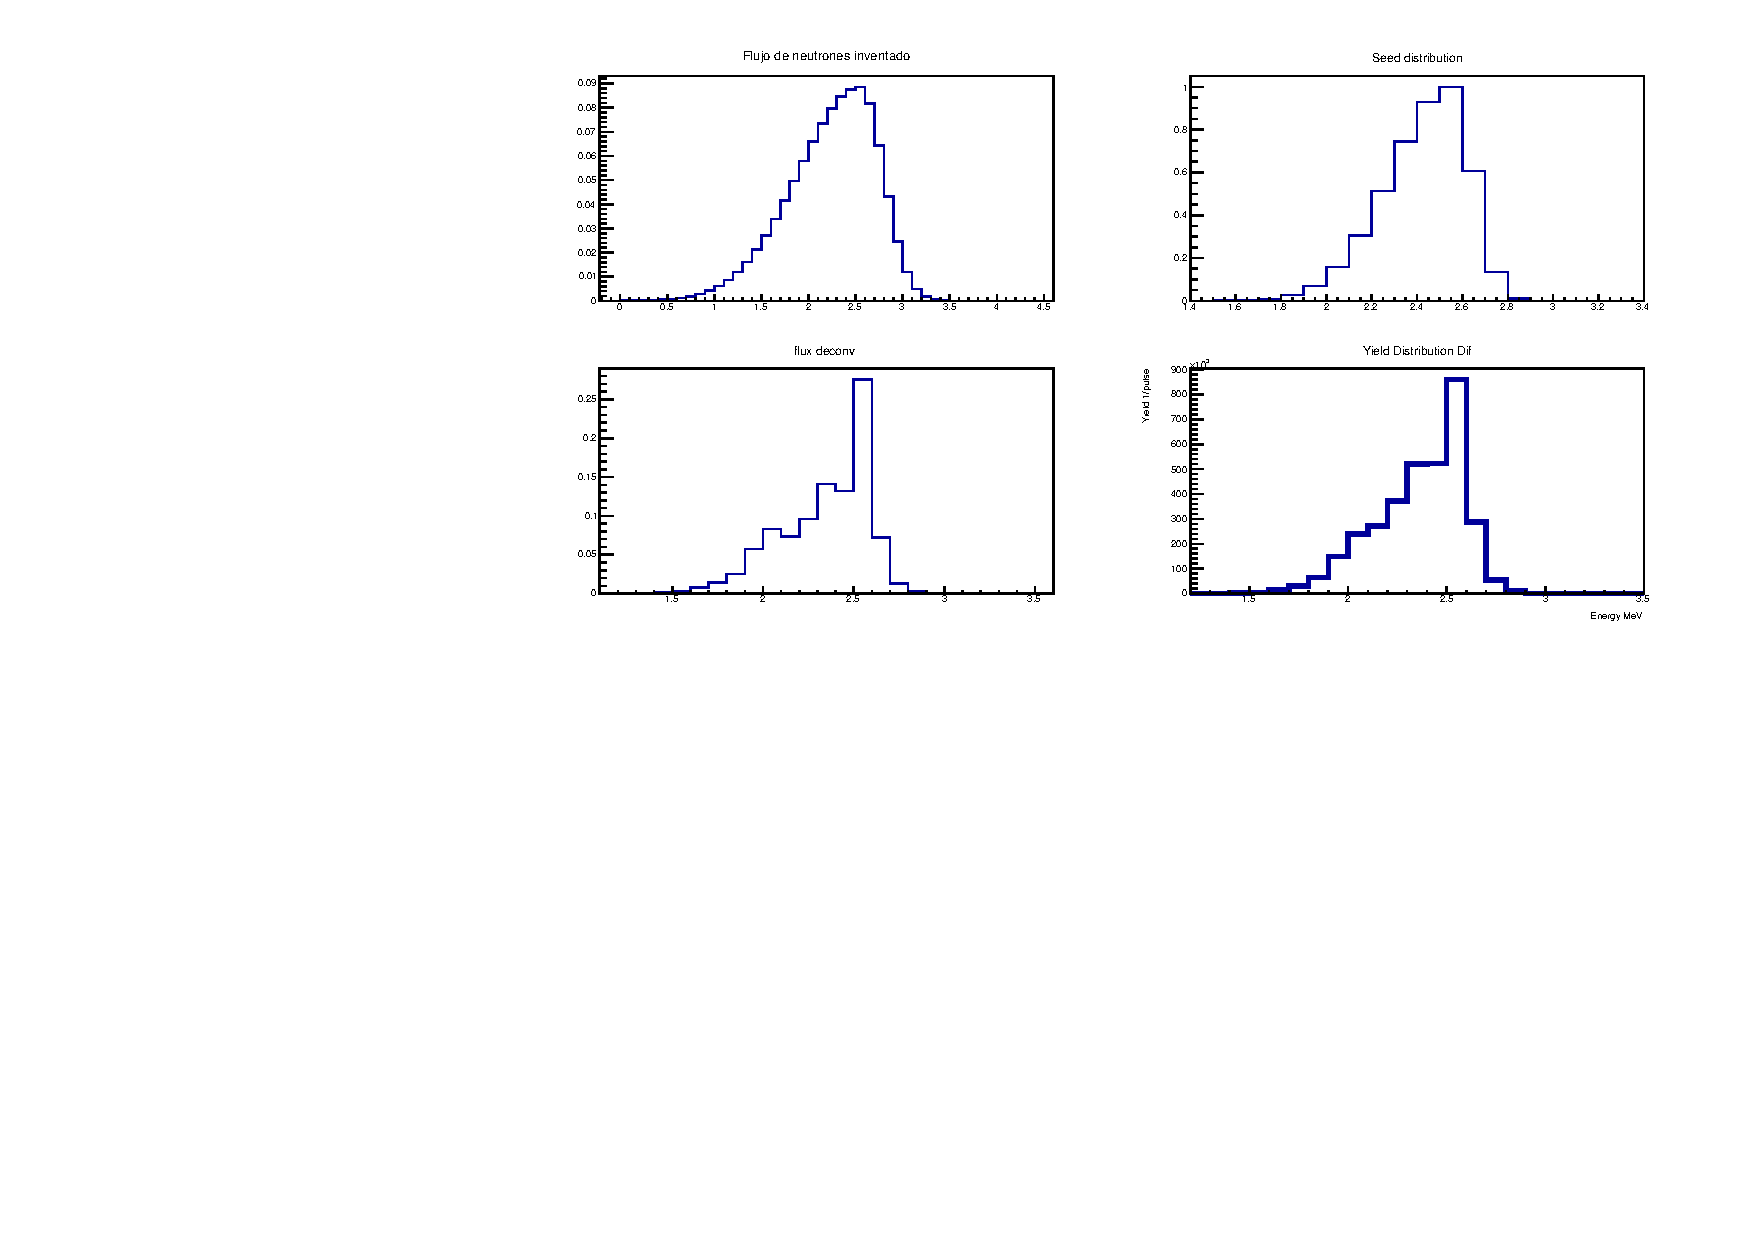
\includegraphics[width=1\textwidth]{img/antes_de_arreglar_Seed.pdf}
    \centering
    \cprotect\caption{Salida antes de arreglar \verb|SeedGenerator()| }
\end{figure}

\begin{figure}[H]
    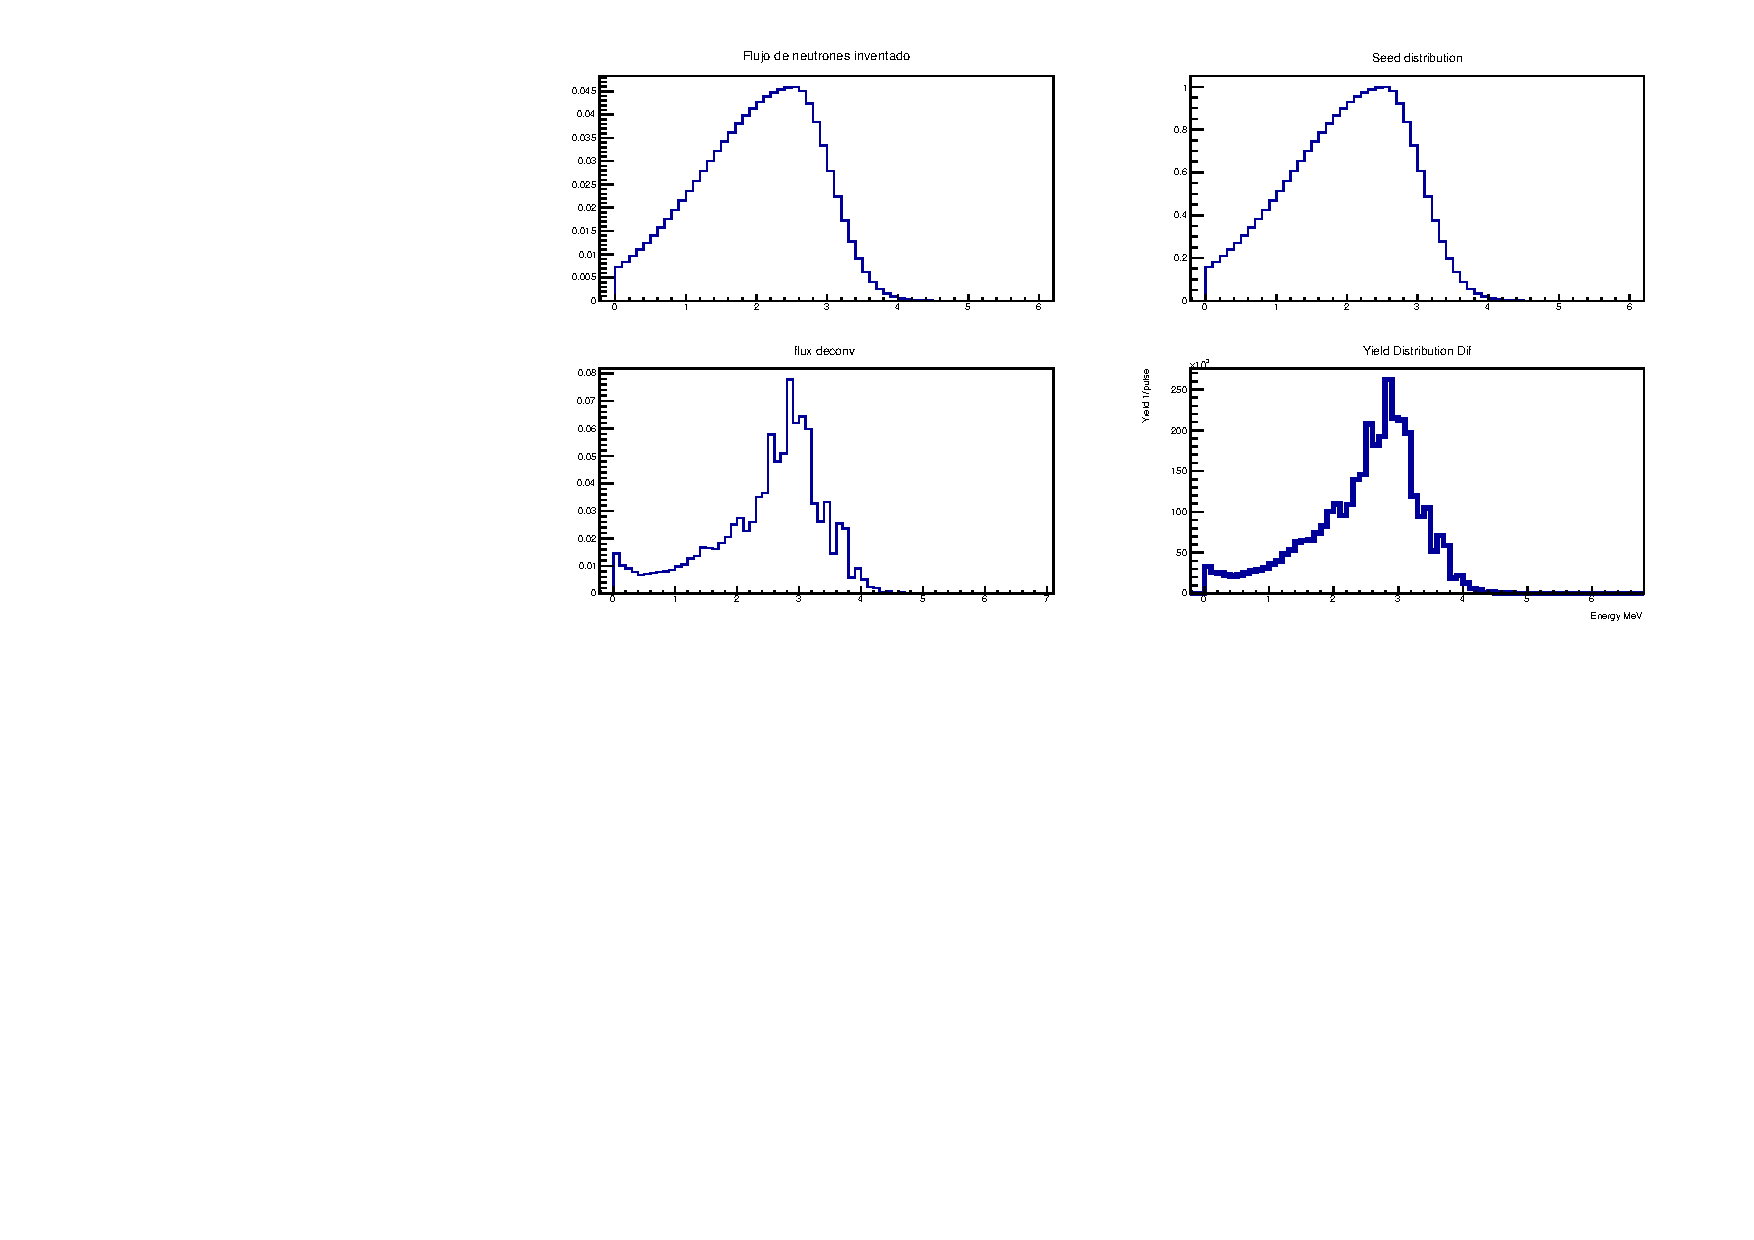
\includegraphics[width=1\textwidth]{img/despues_de_arreglar_Seed.pdf}
    \centering
     \cprotect\caption{Salida después de arreglar \verb|SeedGenerator()| }
\end{figure}

Se cambio el parámetro \verb|dist| de tipo \verb|TString| a tipo \verb|int| en \verb|SeedGenerator()|, ahora $1$ corresponde a $G$ y $2$ a $AG$. Esto para hacer más manejable la conversión a vectores de las lineas del archivo \verb|neutrones_calculados_merge.dat| en la función \verb|ReadDataShot()|. Así, el parámetro \verb|dist| queda como tipo \verb|int| en las funciones:

\verb|void Pretty_EMsimple()|\\
\verb|void Pretty_EMsimple_em1()|\\
\verb|void Test_Unfolding| \\
\verb|TH1D* Test_Unfolding_TH1D()| \\
\verb|void Test_Unfolding_shots()|\\

Además, de esta manera en \verb|void Pretty_EMsimple_em1()|  ahora graficamos de forma correcta el flujo inventado que genera los neutrones calculados, los cuales sirven de entrada para el método EM.
Quedando la línea de código que genera el histograma de flujo inventado como:

\verb| TH1D* flux_inv = Test_Unfolding_TH1D(par1_inv, par2_inv, dist_inv, SIG_L_inv, SIG_R_inv);|

y donde los parámetros vienen de:

\begin{lstlisting}[language=c++]
/*Trabajamos con el vector Neutrons de ReadDataShot*/
	vector<double_t> Neutrons_raw = ReadDataShot("./neutrones_calculados/neutrones_calculados_merge.dat", shot, ndet); /*vector de 12 entradas con toda la info */
	int neutrons_size = Neutrons_raw.size();
	/*Parametros del flujo inventado asociado a un shot*/
	vector<double_t> Neutrons_param(Neutrons_raw.begin()+neutrons_size-5, Neutrons_raw.begin()+neutrons_size);
	std::cout << "Parametros de Neutrones calculados	" << endl;
	std::cout << "n = { ";
    for (Double_t n : Neutrons_param) {
        std::cout << n << ", ";
    }
    std::cout << "}; \n";
	std::cout << std::endl;
	int dist_inv = Neutrons_param[0];
	double_t par1_inv = Neutrons_param[1];
	double_t par2_inv = Neutrons_param[2];
	double_t SIG_L_inv = Neutrons_param[3];
	double_t SIG_R_inv = Neutrons_param[4];
	
	
	/*Neutrones calculados*/
	vector<double_t> Neutrons_cal(Neutrons_raw.begin()+1, Neutrons_raw.begin()+ndet+1);
	N = Neutrons_cal;
\end{lstlisting}

Visualización correcta del flujo inventado para la línea de código:

\verb|pulse.Pretty_EMsimple_em1(15, 1000, 2.5, 0.2,"Dif", 1, 12, 2 ,1.3,0.5);|

\begin{figure}[H]
    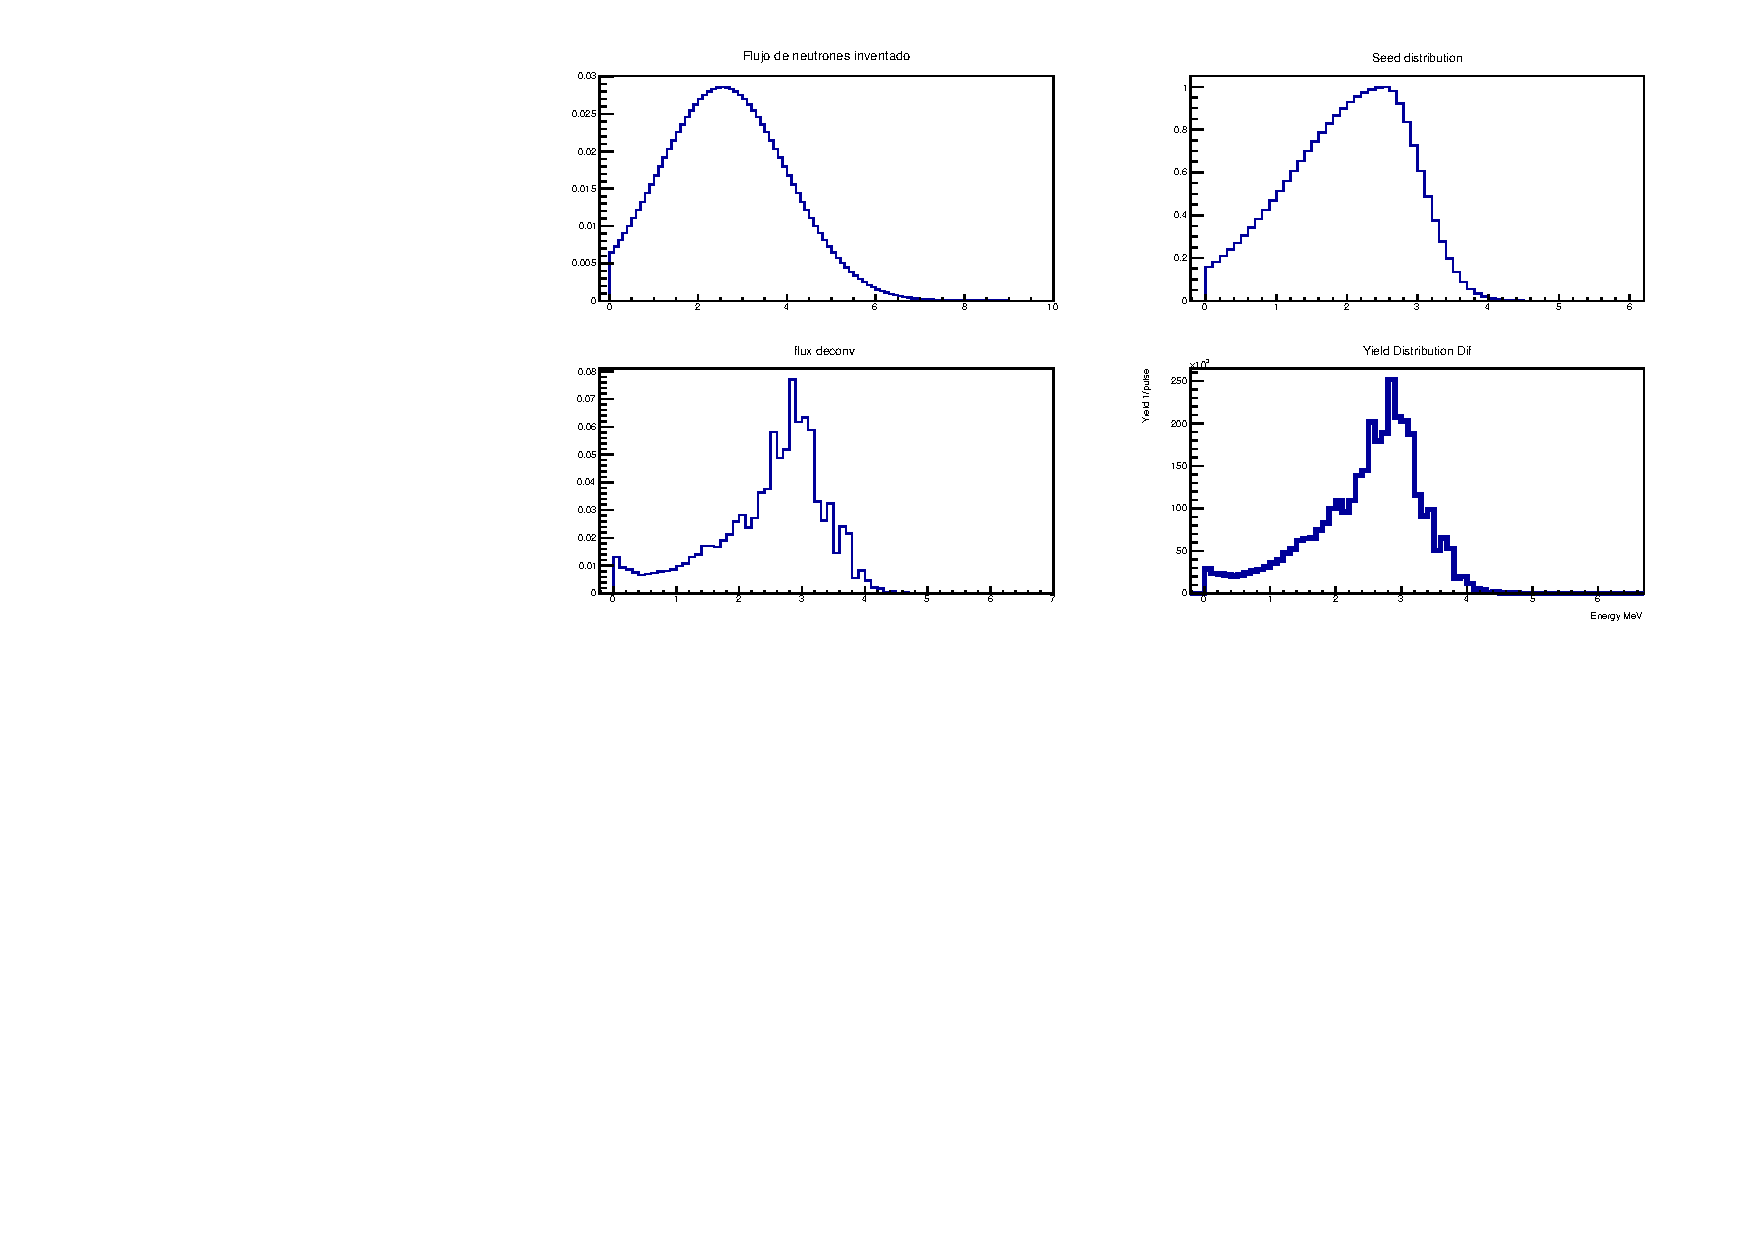
\includegraphics[width=1\textwidth]{img/flux_inventado_arreglado_en_em1.pdf}
    \centering
     \cprotect\caption{Salida después de arreglar los parámetros del flujo inventado en \verb|void Pretty_EMsimple_em1()| }
\end{figure}

\section{2021-12-09}
\label{2021-12-09}
Actualización del repositorio en GitLab con lo mencionado en la entrada anterior (\ref{2021-12-08}) de commit \verb|3c84a7d8| que de acuerdo a GitLab se hicieron: 4 changed files with 306 additions and 90 deletions:

\begin{figure}[H]
    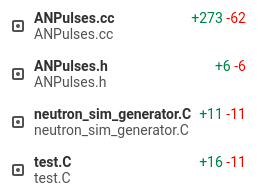
\includegraphics[width=0.3\textwidth]{img/commit_3c84a7d8.png}
    \centering
     \cprotect\caption{Actualización de archivos en el repositorio en Gitlab de commit \verb|3c84a7d8|. }
\end{figure}

Además de estos cambios, se mejoró el algoritmo (\ref{em1}),  para esto, debugeamos esta implementación guardando un archivo de nombre \verb|objets_debug.dat| con todas las variables de entrada de la función \verb|Pretty_EMsimple_em1()|: 

\begin{itemize}

\item[•] \verb|vector<double_t>  N| : Neutrones calculados .
\item[•]\verb|vector<double_t>  Neutrons_raw|: Neutrones calculados raw (con informacion de \# shot, y parámetros del flujo inventado).
\item[•] \verb|Double_t SolAng_Dec1| : Valores de ángulos sólidos por detector.
\item[•]\verb|vector<double_t> Seed| : Flujo semilla
\item[•] \verb|vector<double_t> dE| :Ancho de bin energía
\item[•]\verb|vector<double_t> Flux|  : Flujo diferencial: (Flujo semilla)/(ancho de bin): $Flux[i] = Seed[i]/dE[i]$
\item[•] \verb|R[i]|  : Entradas de la matriz eficiencias absolutas (``Funciones respuesta'')
\item[•]\verb|R[i]| Entradas de la matriz de eficiencias absolutas luego de reemplazar ceros por $1.E-23$
\end{itemize}

Es importante destacar que para generar correctamente este archivo, en la macro \verb|test.C| tiene que ir nuevamente definido:

\verb|ofstream objets_debug("objets_debug.dat");|

seguido por:

\verb|pulse.Pretty_EMsimple_em1(15, 1000, 2.5, 1.0,"Dif", 1, 12, 2 ,1.3,0.5);|

En la función \verb|Pretty_EMsimple_em1()| también se implementó el guardar un histograma de flujo deconvolucionado por cada paso del algoritmo EM (creando un vector de histogramas), con la idea posterior de producir un canvas donde  se muestre la deformación del flujo  por cada paso del método, esto es, visualizar a la izquierda el flujo inventado y a la derecha de este el flujo en constante actualización por paso. 

\begin{tipt}
\verb|C++|:
\begin{itemize}
\item[•] \verb|vector.size()| cuando el vector no es un puntero
\item[•]  \verb|vector->size()| cuando el vector es un puntero.
\end{itemize}
\end{tipt}

\subsection*{Avance del código en LIN}
Posterior a la actualización anterior, en la CCHEN, continué trabajando en el código, realizando las siguientes actualizaciones:

Se crea una macro de nombre \verb|deconvoluciones.C| con dos funciones:

\begin{itemize}
\item[•] \verb|void neutrones_deconv()| la cuál para distintos disparos, es decir, para distintos flujos inventados, itera el método EM, \verb|Pretty_EMsimple_em1()| para distintos valores de ancho del flujo semilla.
\item[•]\verb|void neutrones_deconv_plot()| grafica un mapa de calor con la comparación del flujo inventado y flujo deconvolucionado, utilizando los valores de archivo \verb|"chi2_test.dat"|
\end{itemize}

En la clase \verb|ANPulses| se creó la función \verb|double_t Xi_Square_em2()| la cuál calcula el $\chi_c^2$ del algoritmo (\ref{em2}), comparando el flujo deconvolucionado con el flujo inventado. Pero en este caso se cambió el denominador $\left(\Delta \Phi_j^{(inv)}\right)^2$ por el cuadrado de la integral del flujo deconvolucionado (ERROR, debería ser la integral del flujo inventado) con una tolerancia del 10\%. A continuación mostramos la implementación de la función nombrada: 

\begin{lstlisting}[language=c++]
double_t ANPulses::Xi_Square_em2(vector<Double_t> N_i, vector<Double_t> N_rec, double_t intgl, double ndet)
{
	double_t xi=0;
	double_t partial_sum=0;
	double_t nprom=0;
	double_t variance=0;
	double_t tolerance = 0.1;

	for (int i = 0; i < ndet; i++){ partial_sum = (N_i[i] - N_rec[i])/(intgl*tolerance); xi += partial_sum*partial_sum; }
	


return xi;
	
}	
	
\end{lstlisting}

Dentro de la función \verb|Pretty_EMsimple_em1()| se crea el archivo de nombre \verb|chi2_test.dat|, el cuál es un archivo de salida para analizar la dependencia del flujo inventado con la semilla en la deconvolucion. Para cada iteración de \verb|Pretty_EMsimple_em1()| en \verb|neutrones_deconv()| se va a agregando una línea en el archivo:

\verb|	ofstream chi2_test("chi2_test.dat", ios_base::app);|

Donde las filas corresponden a columnas con la siguiente información:

\begin{itemize}

\item[•] \verb|shot|: número de disparo
\item[•] \verb|it|: paso de iteración para el cuál se satisface EM1 (\ref{em1})
\item[•] \verb|par2|: ancho del flujo semilla 
\item[•] \verb|par2_inv|: ancho del flujo inventado
\item[•] \verb|chi2_em2|: valor de $\chi_c^2$ del algoritmo EM2 (\ref{EM2})

Ejemplo de la salida:


\begin{lstlisting}[language=c++]
1     1     0.1   0.05  19.2782
1     351   0.5   0.05  53.4334
1     1     0.9   0.05  58.4065
1     990   1.3   0.05  58.634
2     1     0.1   0.15  2.75981
2     1     0.5   0.15  9.16272
...
16    1124  0.9   1.55  0.138689
16    1     1.3   1.55  0.036807
\end{lstlisting}


\end{itemize}


A la salida \verb|"objets_debug.dat"| se le agrega al final, lo siguiente:

\begin{itemize}
\item[•] \verb|vector<double_t> vec_fluxinv|: flujo inventado\
\item[•] \verb|vector<double_t> vec_fluxdeconv|: flujo deconvolucionado

\end{itemize}




\section{Entrada del 2021-12-14}
\label{2021-12-14}

Nueva actualización del repositorio en GitLab con el avance realizado en el laboratorio LIN, sistematizado en la entrada anterior. Además se agregó al \verb|readme| las instrucciones para generar una simulación experimental y poder testear así la dependencia del método con la semilla inicial.


\begin{lstlisting}[language=bash]
...
RUN SIMULATION EXPERIMENT:

root -l

			.L ANPulses.cc++
			.L neutron_sim_generator.C
			neutrones_sim_generator_merge()  # genera los neutrones simulados
			.L deconvoluciones.C
			neutrones_deconv()               #aplicamos eL metodo EM para cada disparo
			neutrones_deconv_plot()          #graficamos un mapa de calor con la comparacion entre flujo deconvolucionado y flujo inventado, donde el eje z es Xi2 de EM2.
\end{lstlisting}

De esta manera, para la primera simulación realizada, se tienen las siguientes condiciones:

Tenemos 64 disparos, donde cada uno corresponde a disparos generados por una distribución inventada de tipo gaussiana centrada en 2.5 y con anchos variables desde 0.01 hasta 0.63 en pasos de 0.01 (ver archivo \verb|neutrones_calculados_merge.dat|). Luego, hasta el disparo 16 anterior, se aplicó la función \verb|Pretty_EMsimple_em1()| con los algoritmos (\ref{EM1}) y (\ref{em2}) implementados. Por cada disparo se itero una semilla inicial del método EM de tipo gaussiano centrada en 2.5 y de ancho variable entre 0.1 y 1.3 en pasos de 0.4.


\begin{lstlisting}[language=c++]
...
void neutrones_deconv(){


ANPulses pulse;

ofstream objets_debug("objets_debug.dat"); //importante para sobreescribir el archivo.
ofstream chi2_test("chi2_test.dat"); //importante para sobreescribir el archivo.

/*Parametros Pretty_EMsimple_em1(): int shot, int steps, double par1, double par2, TString Type, 
 * int rebin, int bin_l, int dist, double_t SIG_L, double_t SIG_R */
//~ pulse.Pretty_EMsimple_em1(15, 1000, 2.5, 1.0,"Dif", 1, 12, 1 ,1.3,0.5);
//~ int num_ite = 16; /*numero de iteraciones*/

for ( int shot=1; shot <= 16; shot++)
		{
			for (double sig=0.1; sig <=1.55; sig+=0.4)
				{
					pulse.Pretty_EMsimple_em1(shot, 1000, 2.5, sig,"Dif", 1, 12, 1 ,1.3,0.5);

				}
		}

}
...
\end{lstlisting}

Luego con el  el archivo de salida de esta función \verb|"chi2_test.dat"| se realiza un mapa de calor, utilizando la función siguiente de la macro \verb|deconvoluciones.C|:

\begin{lstlisting}[language=c++]
...
void neutrones_deconv_plot(){

//~ vector<double_t > Neutrons;
	ifstream file("chi2_test.dat"); 
	vector< vector<double_t>> vectors; /*matriz de disparos*/
	std::string line;
	while (std::getline(file, line))
	{
	  std::istringstream ss(line);
	  std::vector<double_t> new_vec;
	  double_t v;
	  while (ss >> v)                 // populate the new vector hasta donde haya doubles
	  {
		new_vec.push_back(v);
	  }
	  vectors.push_back(new_vec);     // append it to the list of vectors
	}

	
	int vectors_size = vectors.size();
	cout << vectors_size << endl;
	TCanvas *c1    = new TCanvas("c1","c1",600,400);
	TH2F *hcol1 = new TH2F("Xi2","Xi2",15,0,1.5,17,0,1.7);
	//~ float px, py;
	
	for (Int_t i = 0; i < vectors_size; i++)
	{
		//~ for (Int_t j = 2; j <= 3; j++)
		//~ {
				hcol1->Fill(vectors[i][2],vectors[i][3],vectors[i][4]);
				//~ cout << vectors[i][j] << " " << vectors[i][j] ;
		//~ }
		
   }
   hcol1->Draw("COLZ");

}
\end{lstlisting}

resultando el gráfico siguiente (\ref{1simu_exp}):

\begin{figure}[H]
    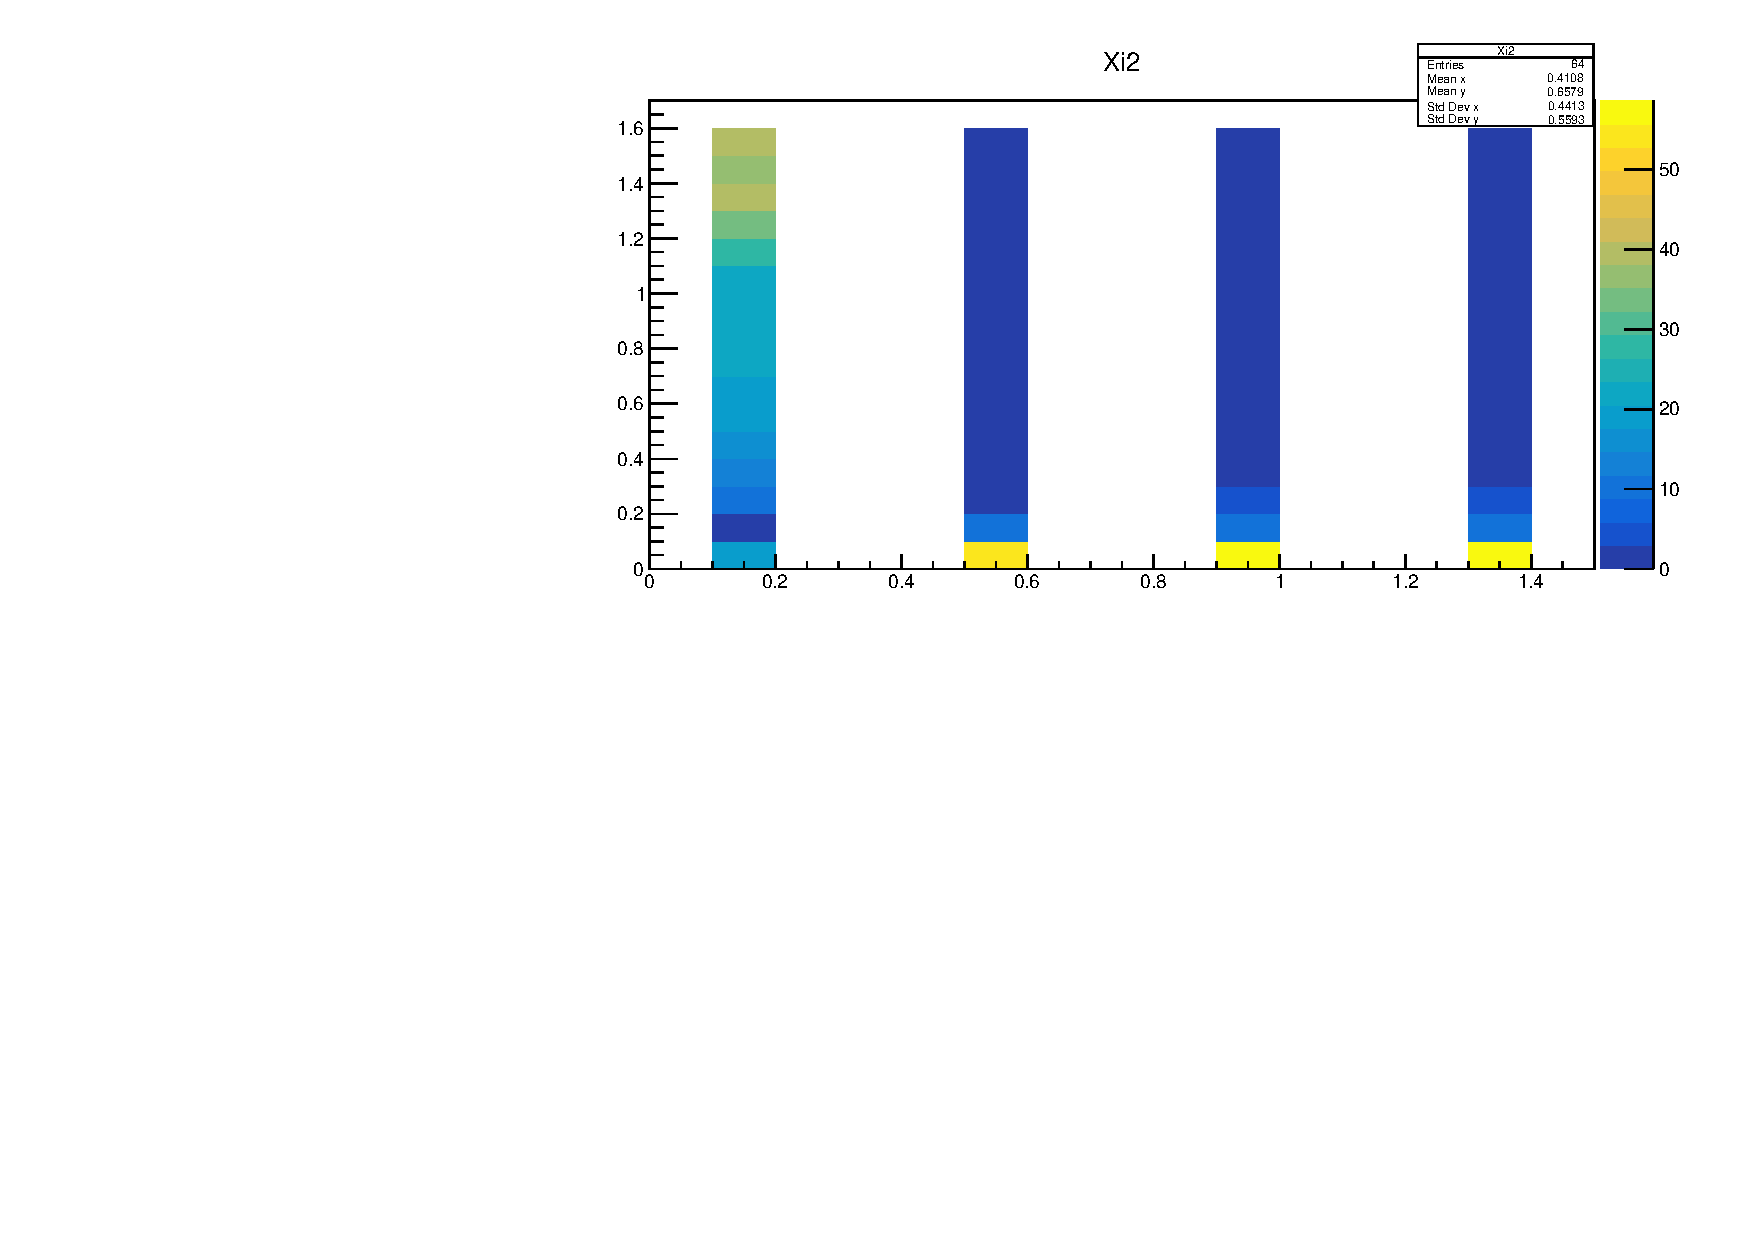
\includegraphics[width=1\textwidth]{img/run1_exp_simulation_64shots.pdf}
    \centering
     \cprotect\caption{Simulación experimental de 64 disparos. Comparación entre el flujo inventado y deconvolucionado usando $\chi_c^2$.}
\label{1simu_exp}
\end{figure}

donde el eje horizontal corresponde a los valores de ancho del flujo semilla del método EM y el eje vertical corresponde a los anchos de los flujos inventados. De esta manera, el eje z corresponde al valor de $\chi_c^2$ que resulta de la comparación entre el flujo inventado y flujo deconvolucionado.

Por lo tanto, a partir de este ejercicio se busca determinar que  grupos de flujo semilla son los mejores en el método EM para variados tipos de flujo inventado, con tal de que el flujo deconvolucionado no se deforme tanto con respecto al flujo inventado (parámetro $\chi_c^2$). De esta manera, en el gráfico (\ref{1simu_exp}) las semillas que cumplen esto deberían formar un \textit{atractor} de valores mínimos en este mapa de calor. 

A su vez, queremos establecer un balance entre el número de pasos (algoritmo \ref{em1}) y la deformación del flujo deconvolucionado (algoritmo \ref{em2}). Por experiencias de trabajos previos (Selene y Pablo) se sabe que a medida que el número de pasos es muy grande, en el flujo resultante del método EM aparecen artefactos matemáticos indeseados y sin relación con la física del problema.

\hightodo{2021-12-14: Generar una clase que inicialice todas las variables que necesito para el algoritmo EM, y así me evito el problema de que al iterar sobre  Pretty EMsimple em1() se produzca un segmentaion fault debido a que no se pueden abrir muchas veces seguidas un archivo .root, como es el caso de las eficiencias intrínsecas.} 

\hightodo{2021-12-14: Establecer un balance entre el número de pasos del método EM y la deformación del flujo deconvolucionado. FMolina sugirió ocupar como parámetro de stop del algoritmo, el producto de  \protect$\chi^2$ ( del algoritmo \ref{em2}) y  \protect$\chi_c^2$.} 

\section{Entrada del 2021-12-20}
\label{2021-12-20}

\begin{tipt}
Valores por defecto de funciones:  Observar que es en la declaración (\verb|clase.h|) solamente que se indica el valor default, no en la implementación (\verb|clase.cc|).
\end{tipt}
\hightodo{2021-12-20: Arreglar el orden de los parámaretros por defecto de la clase ANPulses, ya que estos tienen que estar en la declaración (clase.h) y no en la implementación (clase.cc)}

\section{Entrada del 2021-12-23}
\label{2021-12-23}

Cambios en la clase \verb|ANPulses|. Se agrega \verb|f->Close()| y \verb|delete f| para evitar el break segmentation por abrir muchos archivos \verb|.root| de manera seguida en los loops, en las siguientes funciones:

\begin{itemize}
\item[•] \verb|Test_Unfolding()|: se agrega \verb|f->Close()| y \verb|delete f| 
\item[•]  \verb|Test_Unfolding_TH1D()|: se agrega \verb|f->Close()| y \verb|delete f| 
\item[•]  \verb|Test_Unfolding_shots()|: se agrega \verb|f->Close()| y \verb|delete f| 
\end{itemize}

Se agrega la clase \verb|InitVar| para inicializar las variables de archivos \verb|.root| necesarios para las deconvoluciones. Esta clase contiene cuatro funciones, donde las tres primeras se remueven de la clase \verb|ANPulses| y la última se adapta desde la función \verb|Pretty_EMsimple_em1()| sacando las líneas que componen la función \verb| R_effiAbs()| de una parte de ella.

\begin{itemize}
\item[•] \verb|vector<Double_t> Readfile()|
\item[•] \verb|vector<Double_t> ReadBining()|
\item[•] \verb|Double_t SolidAngle()|
\item[•] \verb|vector<vector<double_t> > R_effiAbs()|: Función que retorna un vector de vectores o matriz de eficiencias absolutas, donde cada entrada corresponde a un vector de eficiencias absolutas asociada a cada sistema de detección.
\end{itemize}

Además en estas funciones se hacen los siguientes cambios que no estaban en \verb|ANPulses|:

\begin{itemize}
\item[•] \verb|vector<Double_t> Readfile()|: 
\begin{itemize}
\item Se cambia \verb|auto f= new TFile(fname)| por \verb|TFile* f = TFile::Open(fname,"read")|
\item Se agrega \verb|delete f| antes de \verb|return R| 
\end{itemize}
\verb|vector<Double_t> ReadBining()| 
\begin{itemize}
\item Se cambia \verb|auto f= new TFile(fname)| por \verb|TFile* f = TFile::Open(fname,"read")|
\item Se agrega \verb|delete f| antes de \verb|return bins| 
\end{itemize}
\end{itemize}

Estos cambios junto con introducir el comando \verb|ulimit -n unlimited| (revisar este comando ya que en realidad debería ser \verb|ulimit -d unlimited| o mejor probar con \verb|ulimit -n 2048| ) antes de correr los programas lograron solucionar el break segmentation fault. Fuentes: \url{https://root-forum.cern.ch/t/too-many-open-files/9237/5}
y \url{https://root-forum.cern.ch/t/file-open-limit/6349/2}.

En \verb|Pretty_EMsimple_em1()| Se comentan los gráficos para disminuir el tiempo de ejecución de los loops. Además las entradas cero del flujo semilla las reemplazamos por $1.0\times 10^{-23}$. También se hacen casos para generar el archivo \verb|chi2_test.dat| de acuerdo a la distribución de los flujo semilla y flujo inventado:

\begin{lstlisting}[language=c++]
...
///////////////////////////////////////////////////
/*Llenamos el archivo chi2_test.dat*/


if( (dist==1) && (dist_inv==1))
	{

					chi2_test << left <<setw(5)<< setfill(' ') << shot << " "
							          <<setw(5) << setfill(' ') << it << " "
							          <<setw(5) << setfill(' ') << par2  << " "  //ancho flujo semilla
							          <<setw(5) << setfill(' ') << par2_inv  << " "  //ancho flujo inventado
							          <<setw(5) << setfill(' ') << chi2_em2 << endl;

	}						          

else if ( (dist==1) && (dist_inv==2))
	{
		chi2_test << left <<setw(5)<< setfill(' ') << shot << " "
							          <<setw(5) << setfill(' ') << it << " "
							          <<setw(5) << setfill(' ') << par2  << " "
							          <<setw(5) << setfill(' ') << SIG_L_inv  << " "
							          <<setw(5) << setfill(' ') << SIG_R_inv  << " "
							          <<setw(5) << setfill(' ') << chi2_em2 << endl;

	}

else if ( (dist==2) && (dist_inv==1))
	{
		chi2_test << left <<setw(5)<< setfill(' ') << shot << " "
							          <<setw(5) << setfill(' ') << it << " "
							          <<setw(5) << setfill(' ') << SIG_L  << " "
							          <<setw(5) << setfill(' ') << SIG_R  << " "
							          <<setw(5) << setfill(' ') << par2_inv  << " "
							          <<setw(5) << setfill(' ') << chi2_em2 << endl;

	}

else

	{
		chi2_test << left <<setw(5)<< setfill(' ') << shot << " "
							          <<setw(5) << setfill(' ') << it << " "
							          <<setw(5) << setfill(' ') << SIG_L  << " "
							          <<setw(5) << setfill(' ') << SIG_R  << " "
							          <<setw(5) << setfill(' ') << SIG_L_inv  << " "
							          <<setw(5) << setfill(' ') << SIG_R_inv  << " "
							          <<setw(5) << setfill(' ') << chi2_em2 << endl;

	}


//////////////////////////////////////////////////
\end{lstlisting}

La macro \verb|neutron_sim_generator.C| se actualiza, agregando descripciones de las funciones implementadas. Además se crea una nueva función llamada \verb|neutrones_sim_generator_merge_fluxinvAG()|, la cuál genera neutrones calculados correspondientes a una distribución de flujo inventada tipo gaussiana asimétrica, donde se varia el ancho del lado izquierdo y derecho, manteniendo el centroide de la distribución en 2.5.

De esta manera, con esta macro podemos generar neutrones calculados para cada sistema de detección en un solo archivo, usando dos tipos de distribuciones.

\begin{table}[H]
\centering
\begin{tabular}{|c|c|}
\hline
\textbf{Función} & \textbf{Descripción}  \\ 
\hline
\verb|neutron_sim_generator_merge_fluxinvG()| & \begin{tabular}{@{}c@{}} Genera neutrones calculados  correspondientes \\ a flujos inventados del tipo gaussiano  donde el \\ parámetro sobre el que se itera corresponde 
al ancho \\ de la gaussiana. Generando entonces \textbf{un} 
 solo archivo: \\ \verb|neutrones_calculados_merge.dat| con los neutrones \\ calculados asociados a un disparo (ancho determinado)\\ y sistema de detección. \end{tabular} \\
\hline
\verb|neutron_sim_generator_merge_fluxinvAG()| & \begin{tabular}{@{}c@{}}Genera neutrones calculados  correspondientes \\ a flujos inventados del tipo gaussiano  asimétrico \\ donde el  parámetro sobre el que se itera corresponde \\ al ancho izquierdo y derecho de dos distribuciones\\  gaussianas. Generando entonces \textbf{un} 
solo archivo: \\ \verb|neutrones_calculados_merge.dat| con los neutrones \\ calculados asociados a un disparo (anchos determinados) \\ y sistema de detección. \end{tabular} \\
\hline
\end{tabular}
\caption{Nuevas funciones.}
\end{table}

Por último se actualiza la macro \verb|deconvoluciones.C|, reestructurando los nombres de sus funciones de la siguiente manera:

\begin{table}[H]
\centering
\begin{tabular}{|c|c|}
\hline
\textbf{Función} & \textbf{Descripción}  \\ 
\hline
\verb|neutrones_deconv_11()| & \begin{tabular}{@{}c@{}}Función que realiza las deconvoluciones\\ utilizando semillas gaussianas simétricas (1)\\ y flujos inventados gaussianos simétricos (1).\\ En ambas distribuciones los pasos de energía para las\\ iteraciones pueden ser ajustados. Como prueba inicial se\\ usaron pasos de de 0.01 o 10 keV. \end{tabular} \\
\hline
\verb|neutrones_deconv_12()| & \begin{tabular}{@{}c@{}}Función que realiza las deconvoluciones\\ utilizando semillas gaussianas simétricas (1)\\ y flujos inventados gaussianos asimétricos (2).\\ En ambas distribuciones los pasos de energía para las\\ iteraciones pueden ser ajustados. Como prueba inicial se\\ usaron pasos de de 0.05 o 50 keV \end{tabular} \\
\hline
\verb|neutrones_deconv_21()| & \begin{tabular}{@{}c@{}}Función que realiza las deconvoluciones\\ utilizando semillas gaussianas asimétricas (2)\\ y flujos inventados gaussianos simétricos (1).\\ En ambas distribuciones los pasos de energía para las\\ iteraciones pueden ser ajustados. Como prueba inicial se\\ usaron pasos de de 0.05 o 50 keV para la primera\\  y pasos de 0.01 0 10 keV para la segunda. \end{tabular} \\
\hline
\end{tabular}
\caption{Actualización del nombre de las funciones.}
\end{table}

Se actualizan y agregan también funciones que realizan mapas de calor con los valores de las deconvoluciones:

\begin{table}[H]
\centering
\begin{tabular}{|c|c|}
\hline
\textbf{Función} & \textbf{Descripción}  \\ 
\hline
\verb|neutrones_deconv_plot()| & \begin{tabular}{@{}c@{}} Función que realiza el grafico de mapa de calor \\ de $\chi_c^2$ en función de los \\ anchos del flujo semilla (gaussiano) y flujo\\ inventado (gaussiano). \end{tabular} \\
\hline
\verb|neutrones_deconv_plotSteps()| & \begin{tabular}{@{}c@{}} Función que realiza el grafico de mapa de calor\\ de pasos que le toma en cumplir al\\ algoritmo em1 (\ref{em1}) en quebrar: $N<\chi^2 $. \\ Esto en función de los anchos del flujo semilla\\ (gaussiano) y flujo inventado (gaussiano). \end{tabular} \\
\hline
\verb|neutrones_deconv_plot_11()| & \begin{tabular}{@{}c@{}} Función que realiza el grafico de mapa de calor\\ de $\chi_c^2$ (pad 11) y de pasos que le toma en cumplir al\\ algoritmo em1 (\ref{em1}) en quebrar: $N<\chi^2 $ (pad 12). \\ Esto en función de los anchos del flujo semilla\\ (gaussiano) y flujo inventado (gaussiano). \\
Luego en los pad 21 y pad 22, se muestran\\ los mismos graficos anteriores pero\\ en escala logarítmica: \verb|gpad->SetLogz()|\end{tabular}\\
\hline
\verb|neutrones_deconv_plot_21()| & \begin{tabular}{@{}c@{}} Función que realiza el grafico de mapa de calor\\ de $\chi_c^2$ (pad 11) y de pasos que le toma en cumplir al\\ algoritmo em1 (\ref{em1}) en quebrar: $N<\chi^2 $ (pad 12). \\ Esto en función de los anchos del flujo semilla\\ (gaussiano asimetrico) y flujo inventado (gaussiano). \\
Luego en los pad 21 y pad 22, se muestran\\ los mismos graficos anteriores pero\\ en escala logarítmica: \verb|gpad->SetLogz()|\end{tabular}\\
\hline
\end{tabular}
\caption{Funciones que realizan graficos de las deconvoluciones.}
\label{neutrones_deconv_plot_1}
\end{table}

Por último se agregan al repositorio los archivos siguientes: 

\begin{itemize}
\item[•]\verb|chi2_test_1-149_fluxseed_G_fluxinv_G.dat|
\item[•]\verb|chi2_test_1-196_fluxseed_G_fluxinv_AG.dat|
\item[•]\verb|neutrones_calculados/neutrones_calculados_merge_fluxinv_AG.dat|
\end{itemize}


\subsection*{Reunión con los profesores Francisco Molina y Víctor Múñoz. (4ta)} 
Se muestran los avances, en específico el gráfico de la simulación \verb|neutrones_deconv_plot_11()|. El profesor Víctor sugirió utilizar un algoritmo genético para encontrar las mejores semillas para el método EM. Para esto, los parámetros de las distribuciones semilla que tendremos en consideración serán el centroide, ancho e inclinación. Dio como consejo explorar esta posibilidad en un plazo de dos semanas. 

Estas simulaciones experimentales (loops), me darán una idea del error de $\sigma_0$, es decir, me permitirán tomar una decisión para los anchos del flujo semilla, de tal manera que sean los que mejor se ajustan al método EM, para variados rangos de ancho del flujo inventado.

También en la discusión, se habló de realizar una exploración del efecto de la variación del centroide, tanto en el flujo semilla como en el flujo inventado. Esto de la manera en que se ha venido realizando, es decir, usando los loops.

El profesor Víctor habló también de realizar pruebas del método con neutrones medidos del experimento e ir viendo que resultados se obtienen para ciertos valores de semilla. La idea es comparar el número de neutrones deconvolucionados con los neutrones medidos. Para lograr esto, antes se necesita calcular el valor de área de un pulso single de un neutrón, valor que se obtiene de las mediciones con fuente de calibración y el sistema de adquisición en modo trigger interno. Por lo que necesitamos convertir estos archivos .root usando el briken offline.

Del gráfico mostrado, el profesor Víctor sugirió normalizar el gráfico de $\chi_c^2$ en función de los anchos de los flujos semilla e inventado, es decir, dividir por el mayor valor encontrado de $\chi_c^2$. Lo mismo para el gráfico de pasos. Sin embargo el profesor Francisco comentó que tal vez para este último no sea tan necesario.

El profesor Francisco, habló de hacer pruebas variando el valor de la tolerancia en $\chi_c^2$, que para las simulaciones hasta ahora, corresponde a un 10\% del valor de la integral del flujo inventado. Entonces, se sugirió tomar valores de 10\%, 5\% y 1\%, de esta manera, se espera que en el gráfico de $\chi_c^2$, la diagonal se vaya cerrando a medida que disminuye el valor de la tolerancia.

\emph{\textbf{Se propuso tener un bosquejo del proyecto de tesis para el 20 de enero.}}

\emph{La quinta reunión quedó agendada para el 6 de enero a las 10 am.}
\section{Entrada del 2021-12-28}
\label{2021-12-28}

Se actualiza el repositorio \verb|class-anpulses| de GitLab con los cambios descritos en la entrada anterior (\ref{2021-12-23}).


\section{Entrada del 2021-12-30}
\label{2021-12-30}

Se termina de actualizar el repositorio \verb|class-anpulses| de GitLab con los cambios descritos en la entrada (\ref{2021-12-23}).

\section{Entrada del 2022-01-03}
\label{2022-01-03}

A continuación describiremos y presentaremos los resultados de las simulaciones experimentales realizadas hasta ahora:

\subsection*{Simulación 11}

Instrucciones para su ejecución:

\begin{itemize}
\item \verb|root -l|
\item \verb|.L InitVar.cc++|
\item \verb|.L ANPulses.cc++|
\item \verb|.L neutron_sim_generator.C|
\item \verb|neutron_sim_generator_merge_fluxinvG()|: Se genera el archivo \verb|neutrones_calculados_merge.dat| con los neutrones calculados asociados a un disparo (ancho determinado) y sistema de detección. Los pasos de ancho para el flujo corresponden a 0.01 o 10 keV, com un máximo de 1.49.
\item \verb|.L deconvoluciones.C|
\item \verb|neutrones_deconv_11()|: 
Input: \verb|neutrones_calculados_merge.dat| Output:  \verb|chi2_test.dat|.

Función que realiza las deconvoluciones utilizando semillas gaussianas simétricas (1) y flujos inventados gaussianos simétricos (1). En ambas distribuciones los pasos de energía para las iteraciones pueden ser ajustados. Como prueba inicial se usaron pasos de de 0.01 o 10 keV para ambos flujos. Se genera entonces el archivo \verb|chi2_test.dat| donde los datos de las columnas corresponden a los explicados en la entrada del (\ref{2021-12-09}).
\item \verb|neutrones_deconv_plot_11()|: Input: \verb|chi2_test.dat| Output: Salida gráfica de root.

Ver tabla (\ref{neutrones_deconv_plot_1})
\end{itemize}

El gráfico generado es el siguiente: 

\begin{figure}[H]
    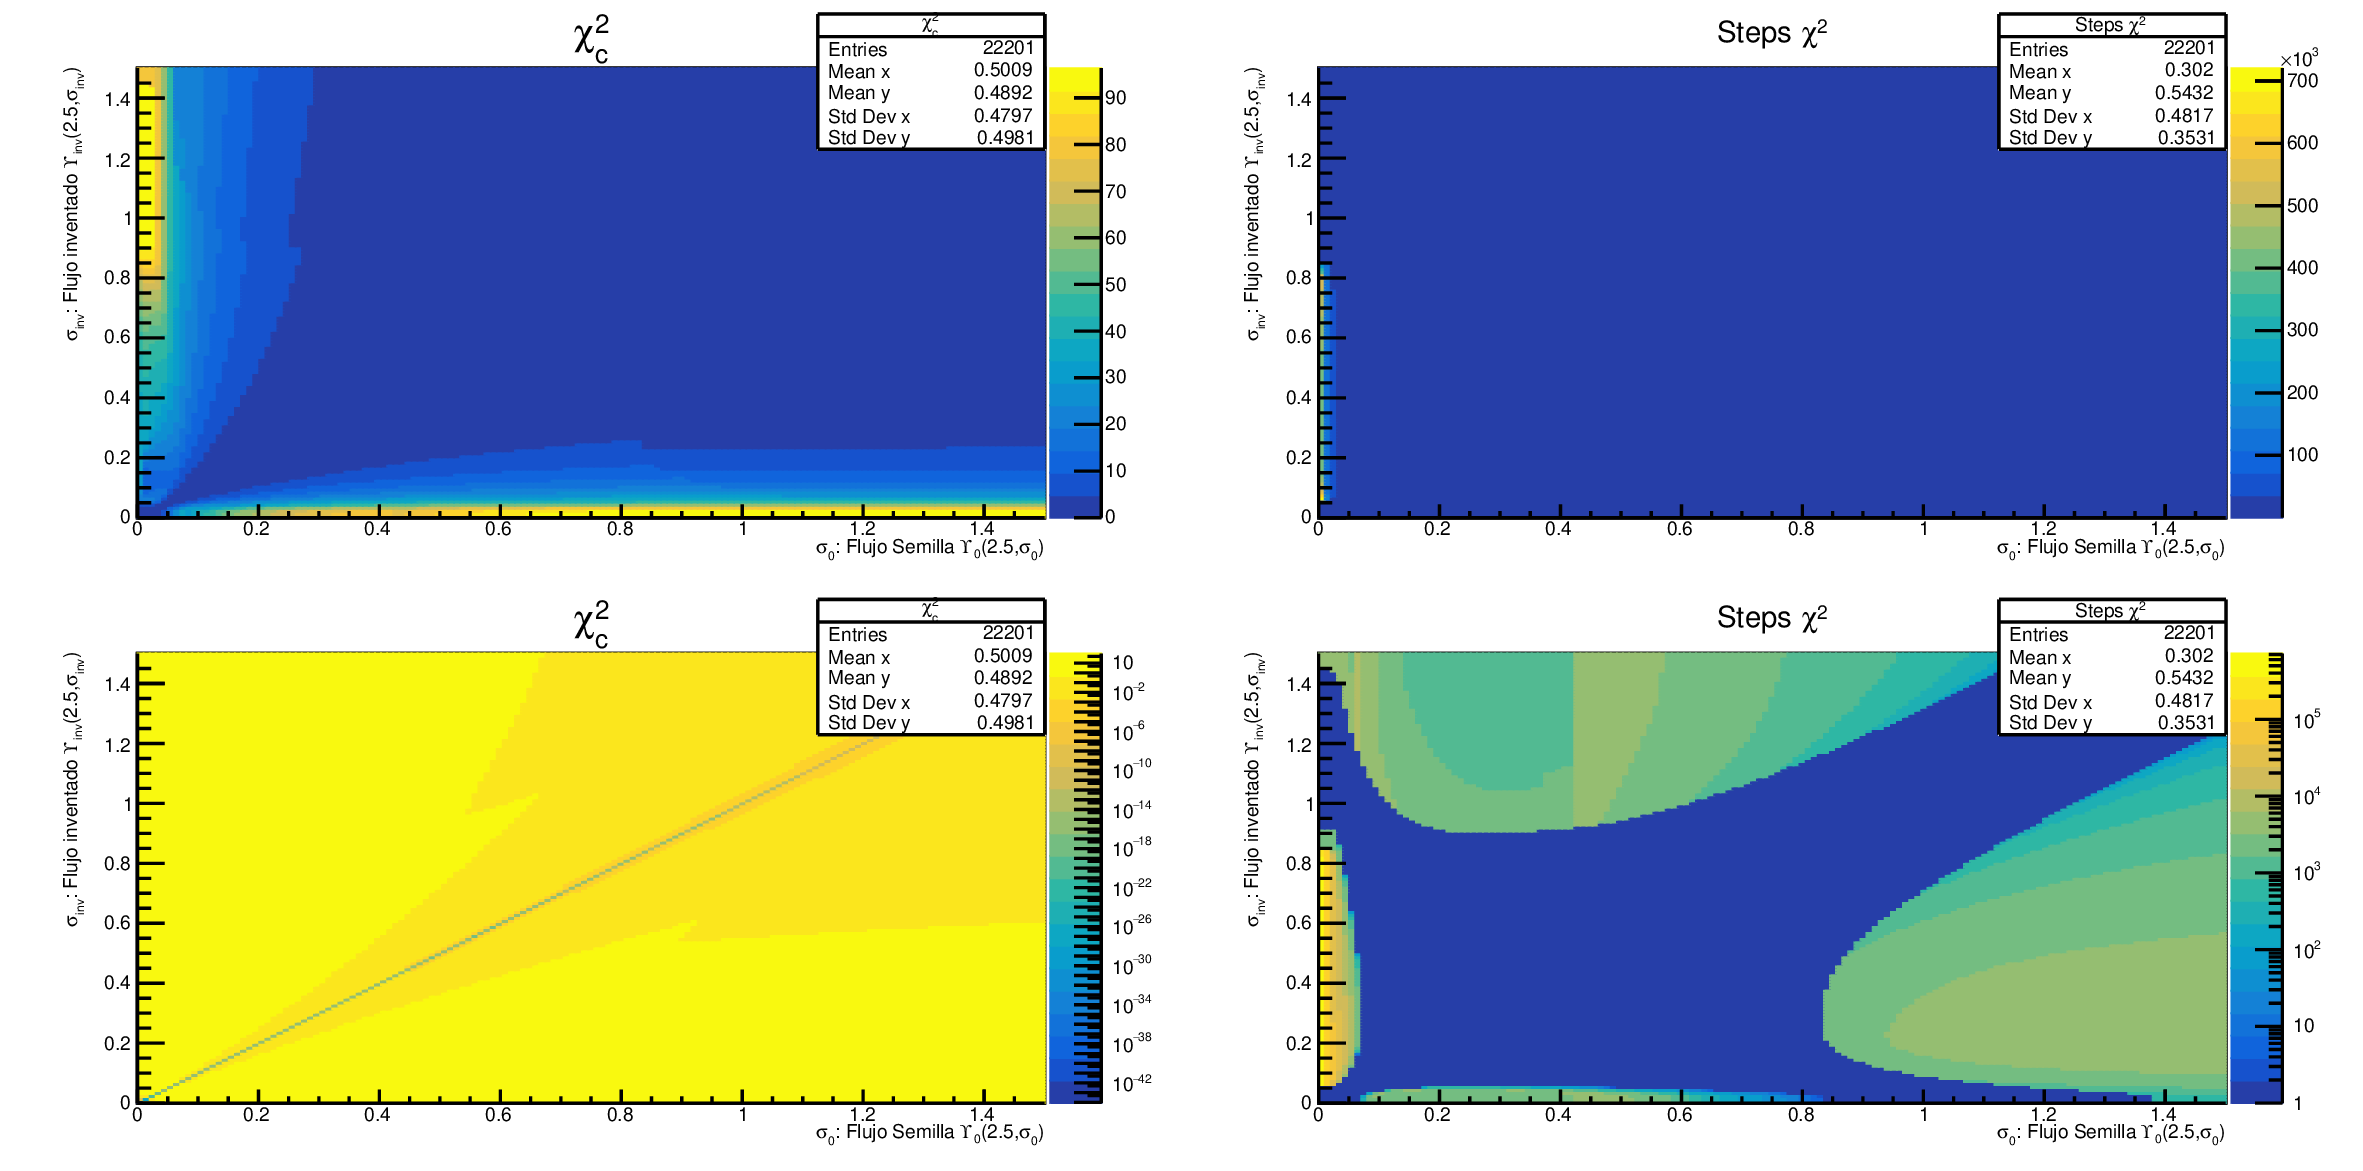
\includegraphics[width=1.\textwidth]{img/chi2_test_1-149_fluxseed_G_fluxinv_G_11.png}
    \centering
     \cprotect\caption{Simulación experimental de 149 disparos. Comparación entre el flujo inventado y deconvolucionado usando $\chi_c^2$.}
\label{neutrones_deconv_plot_11}
\end{figure}


Donde los pads (21) y (22) de la Fig. \ref{neutrones_deconv_plot_11} corresponden a representaciones en escala logarítmica en el eje z de los respectivos gráficos superiores.
Podemos manipular cada pad del gráfico mediante el menú de root, usando las funciones de la clase \verb|TH2F| llamadas \verb|SetMaximum()| y \verb|SetMinimum()|, que tienen por definición (\url{https://root.cern/doc/v612/TH1_8h_source.html#l00390}):

\begin{lstlisting}[language=c++]
    /*
     * Set the minimum / maximum value for the Y axis (1-D histograms) or Z axis (2-D histograms)
     *   By default the maximum / minimum value used in drawing is the maximum / minimum value of the histogram
     * plus a margin of 10%. If these functions are called, the values are used without any extra margin.
     */
    virtual void     SetMaximum(Double_t maximum = -1111) { fMaximum = maximum; }; // *MENU*
    virtual void     SetMinimum(Double_t minimum = -1111) { fMinimum = minimum; }; // *MENU*
\end{lstlisting}
			
Por ejemplo, el el pad (12) hacemos:

\begin{itemize}
\item Click derecho sobre la imagen
\item Seleccionamos la función \verb|SetMinimum|
\item Se abre una ventana, donde ingresamos el valor de 100 y le damos OK.
\end{itemize}			

Obteniendo el siguiente resultado:

\begin{figure}[H]
    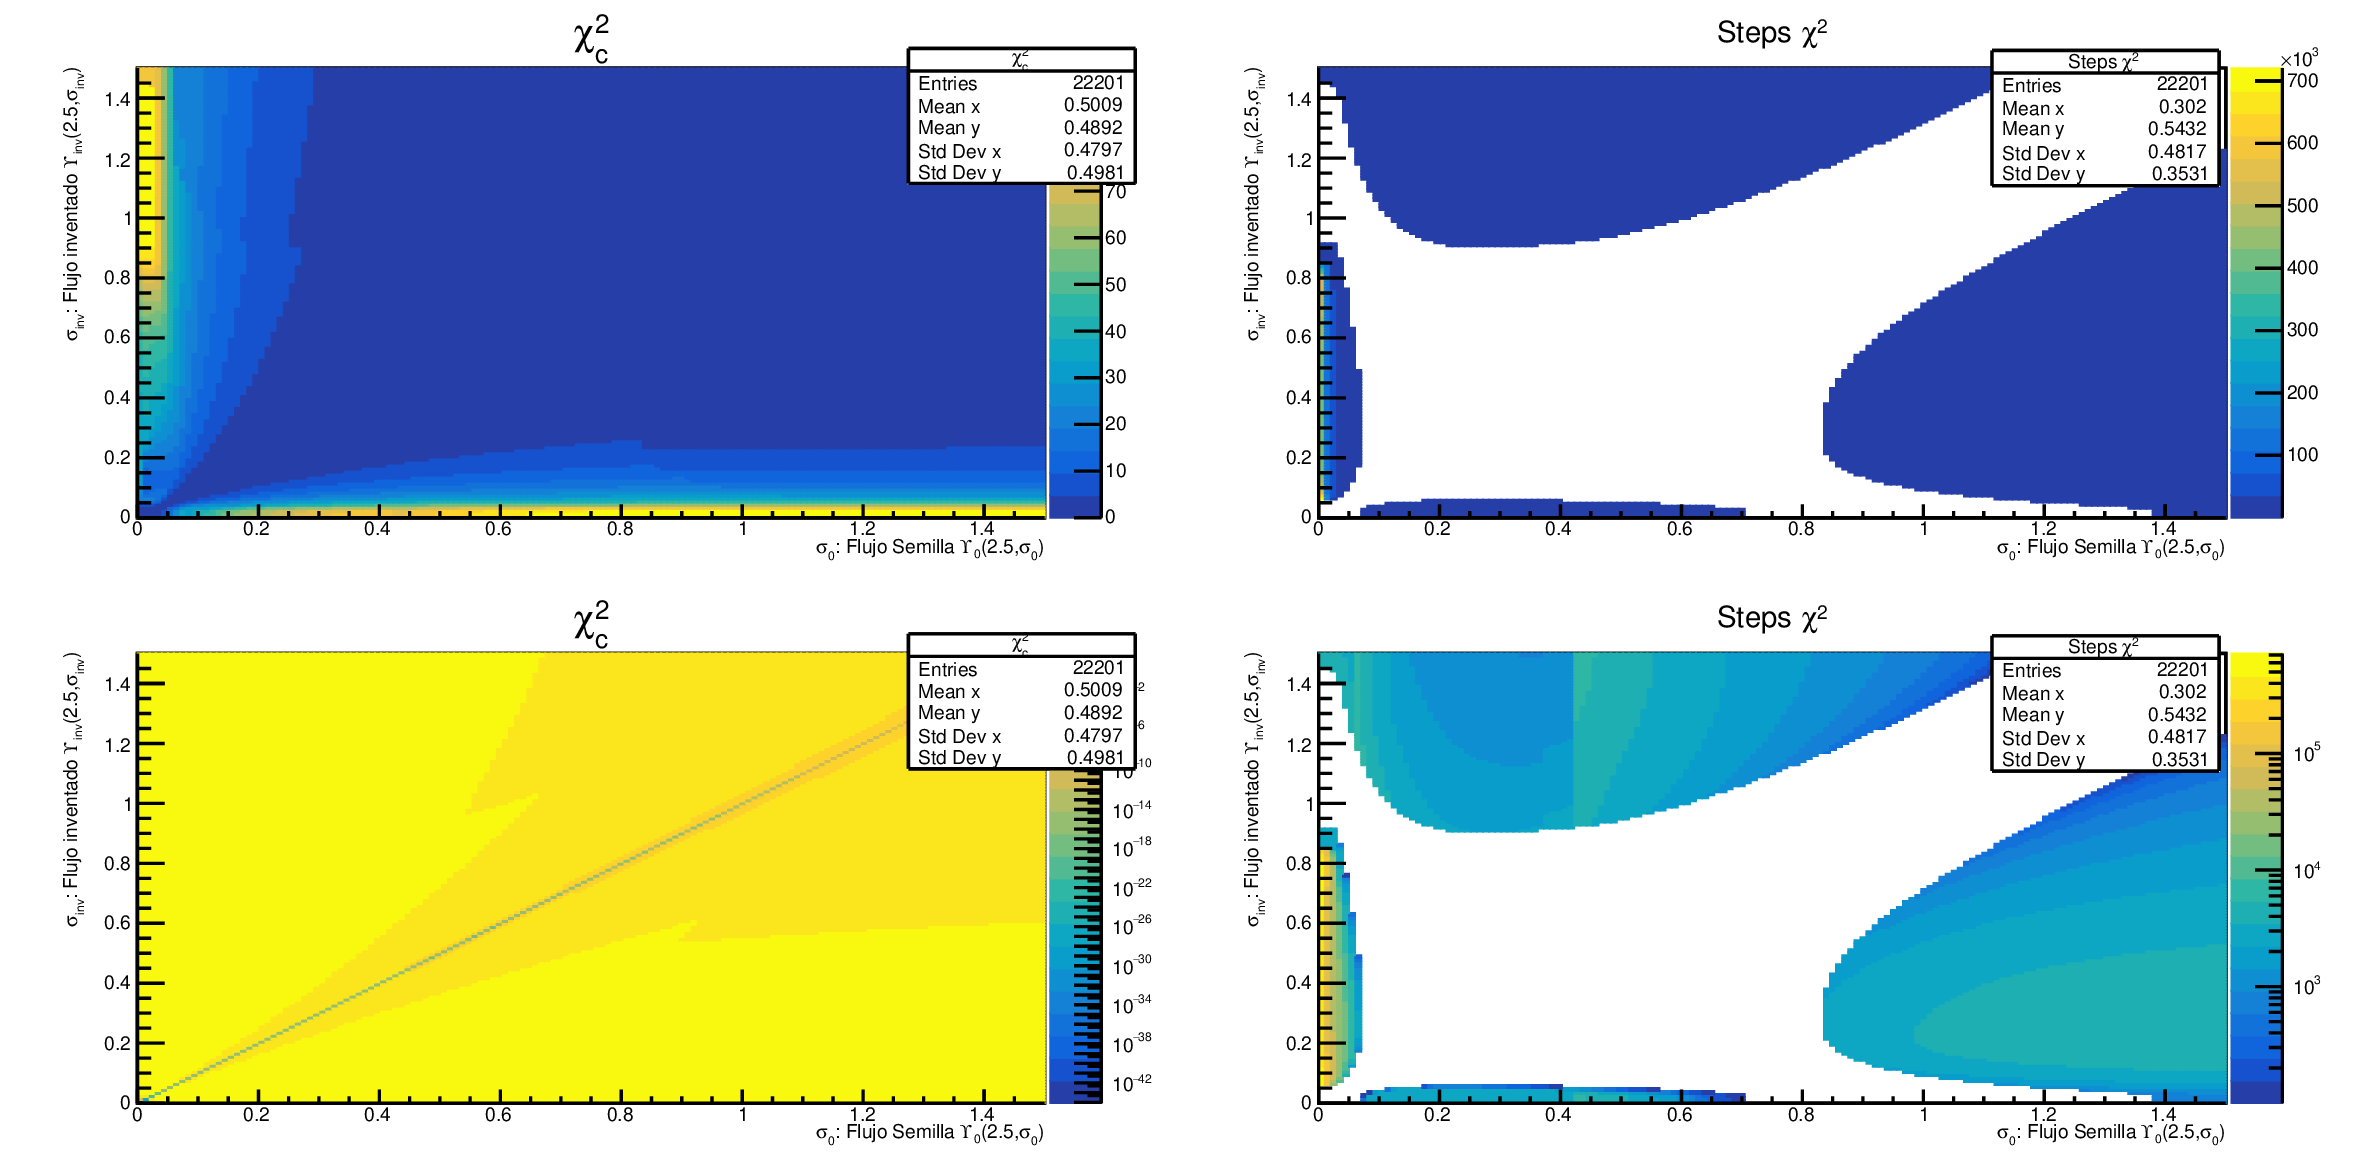
\includegraphics[width=1.\textwidth]{img/chi2_test_1-149_fluxseed_G_fluxinv_G_11_SetMinimum100.png}
    \centering
     \cprotect\caption{Grafico \ref{neutrones_deconv_plot_11} donde el SetMinimum() es 100} 
\label{neutrones_deconv_plot_11_SetMinimum100}
\end{figure}

Donde se muestran los valores de pasos que son mayores a 100, y los menores se eliminan.

Otro ejemplo es el siguiente, donde se estableció el máximo (\verb|SetMaximum|) en 3000 para el pad (12):

\begin{figure}[H]
    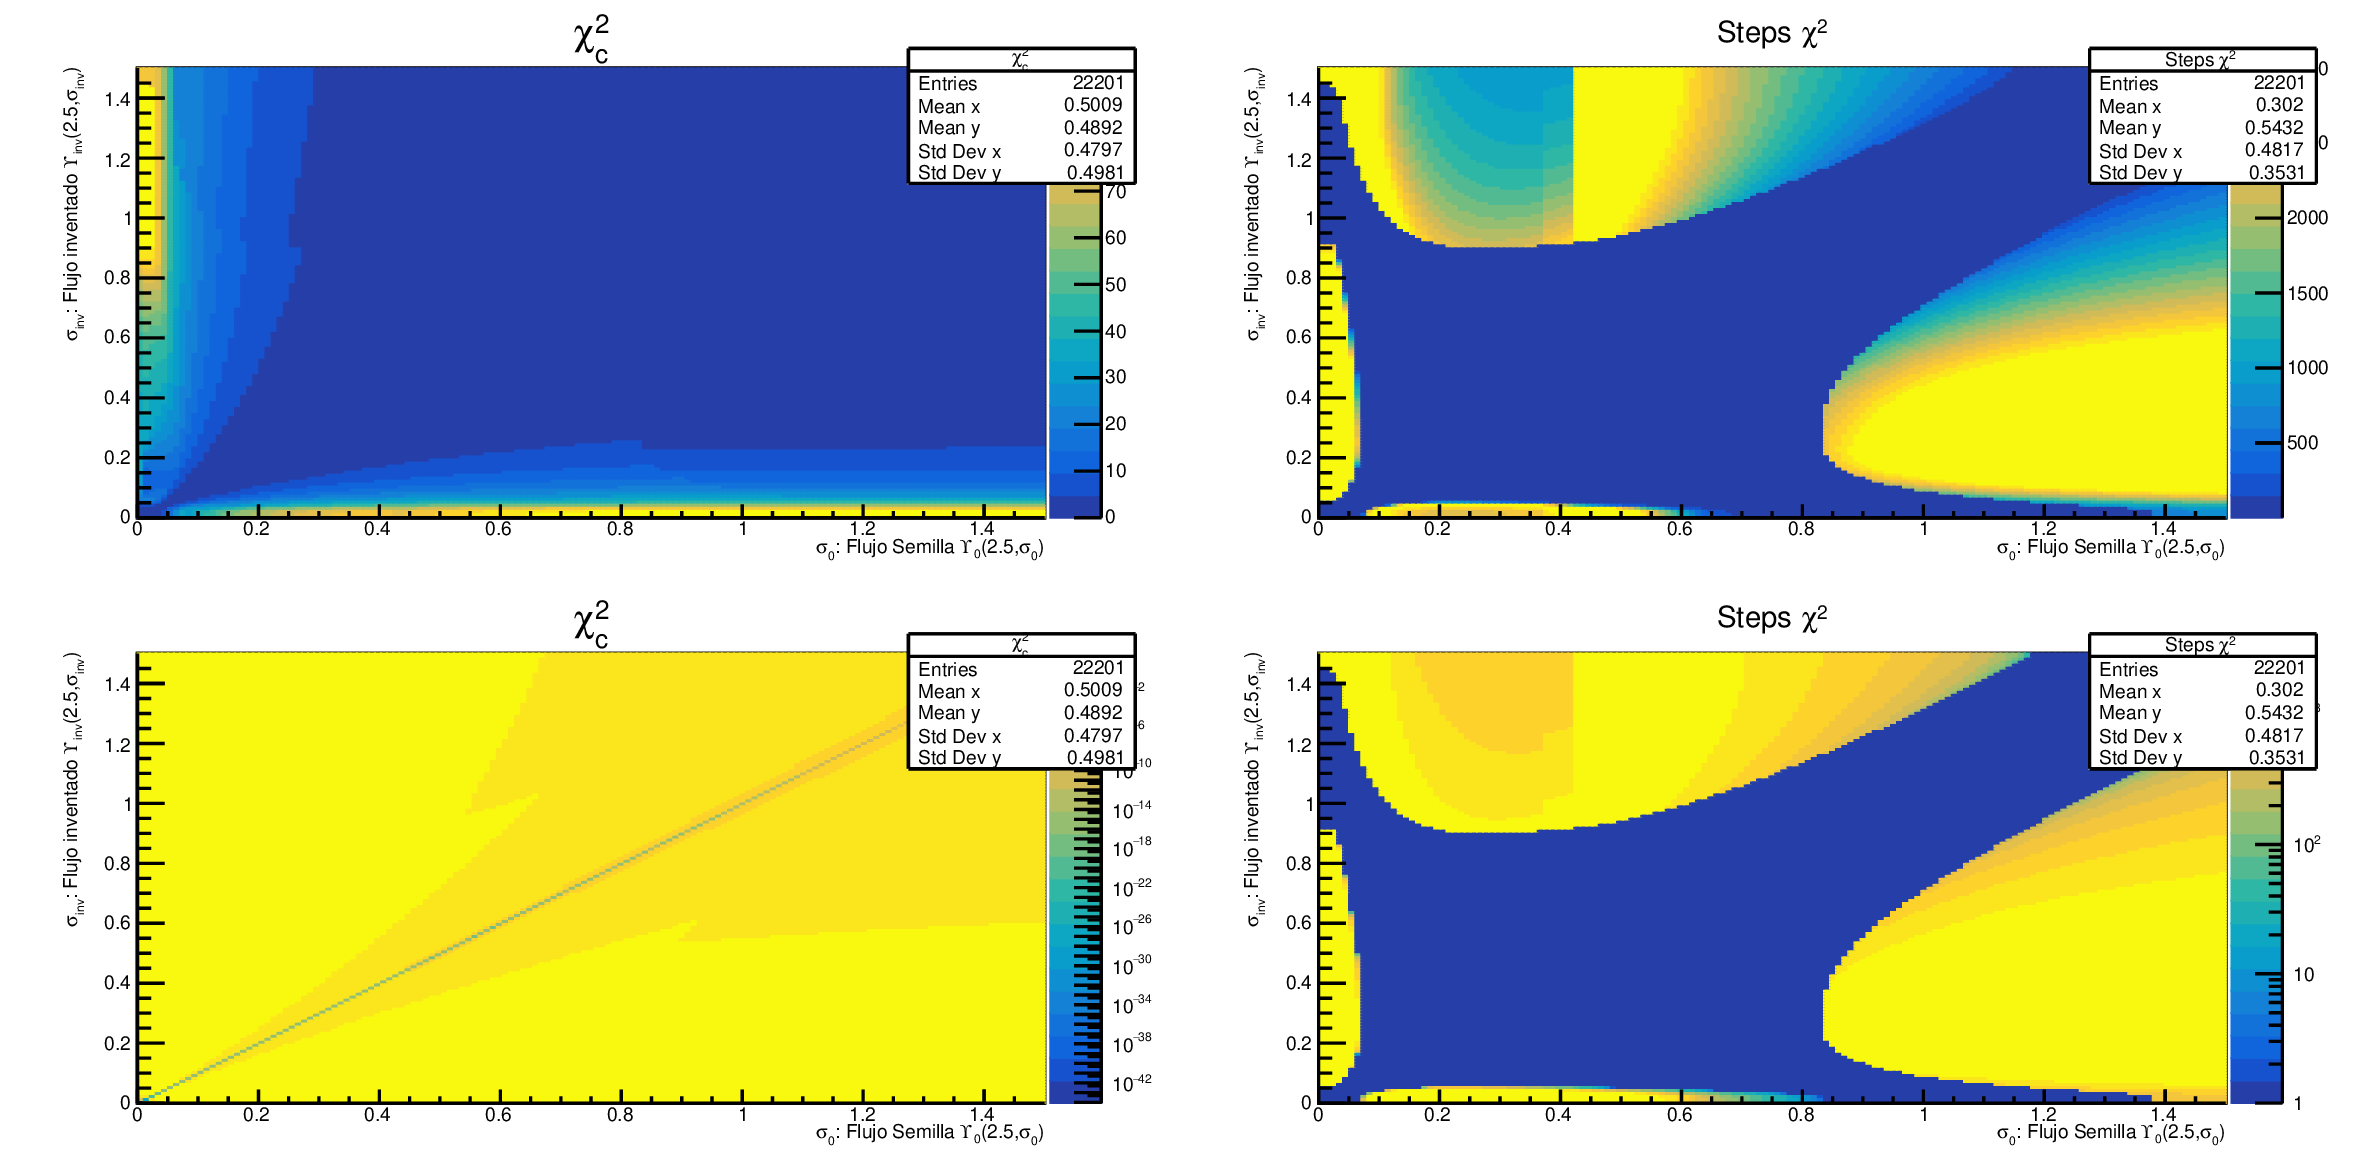
\includegraphics[width=1.\textwidth]{img/chi2_test_1-149_fluxseed_G_fluxinv_G_11_SetMaximum3e3.png}
    \centering
     \cprotect\caption{Grafico \ref{neutrones_deconv_plot_11} donde el SetMaximum() es 3000} 
\label{neutrones_deconv_plot_11_SetMaximum3000}
\end{figure}

\section{Entrada del 2022-01-04}
\label{2022-01-04}

\subsection*{Simulación 21}

Instrucciones para su ejecución:

\begin{itemize}
\item \verb|ulimit -n 30000|: donde 29204 es el número total de filas en \verb|chi2_test_deconv_21.dat|
\item \verb|root -l|
\item \verb|.L InitVar.cc++|
\item \verb|.L ANPulses.cc++|
\item \verb|.L neutron_sim_generator.C|
\item \verb|neutron_sim_generator_merge_fluxinvG()|: Se genera el archivo \verb|neutrones_calculados_merge.dat| con los neutrones calculados asociados a un disparo (ancho determinado) y sistema de detección. Los pasos de ancho para el flujo corresponden a 0.01 o 10 keV, con un máximo de 1.49.
\item \verb|.L deconvoluciones.C|
\item \verb|neutrones_deconv_21()|: 
Input: \verb|neutrones_calculados_merge.dat| Output:  \verb|chi2_test.dat|.

Función que realiza las deconvoluciones utilizando semillas gaussianas asimétricas (2) y flujos inventados gaussianos simétricos (1). En ambas distribuciones los pasos de energía para las iteraciones pueden ser ajustados. Se usaron pasos de 0.05 o 50 keV para las anchos izquierdo y derecho de los flujos semilla asimétricos (como máximo 0.7 por cada lado). Se genera entonces el archivo \verb|chi2_test.dat| donde los datos de las columnas corresponden a (visto como vector en c++) a lo mostrado en la entrada del \ref{2021-12-23}.
\item \verb|neutrones_deconv_plot_21()|: Input: \verb|chi2_test.dat| Output: Salida gráfica de root.

Ver tabla (\ref{neutrones_deconv_plot_1})
\end{itemize}

De esta manera, el gráfico generado es el siguiente:

\begin{figure}[H]
    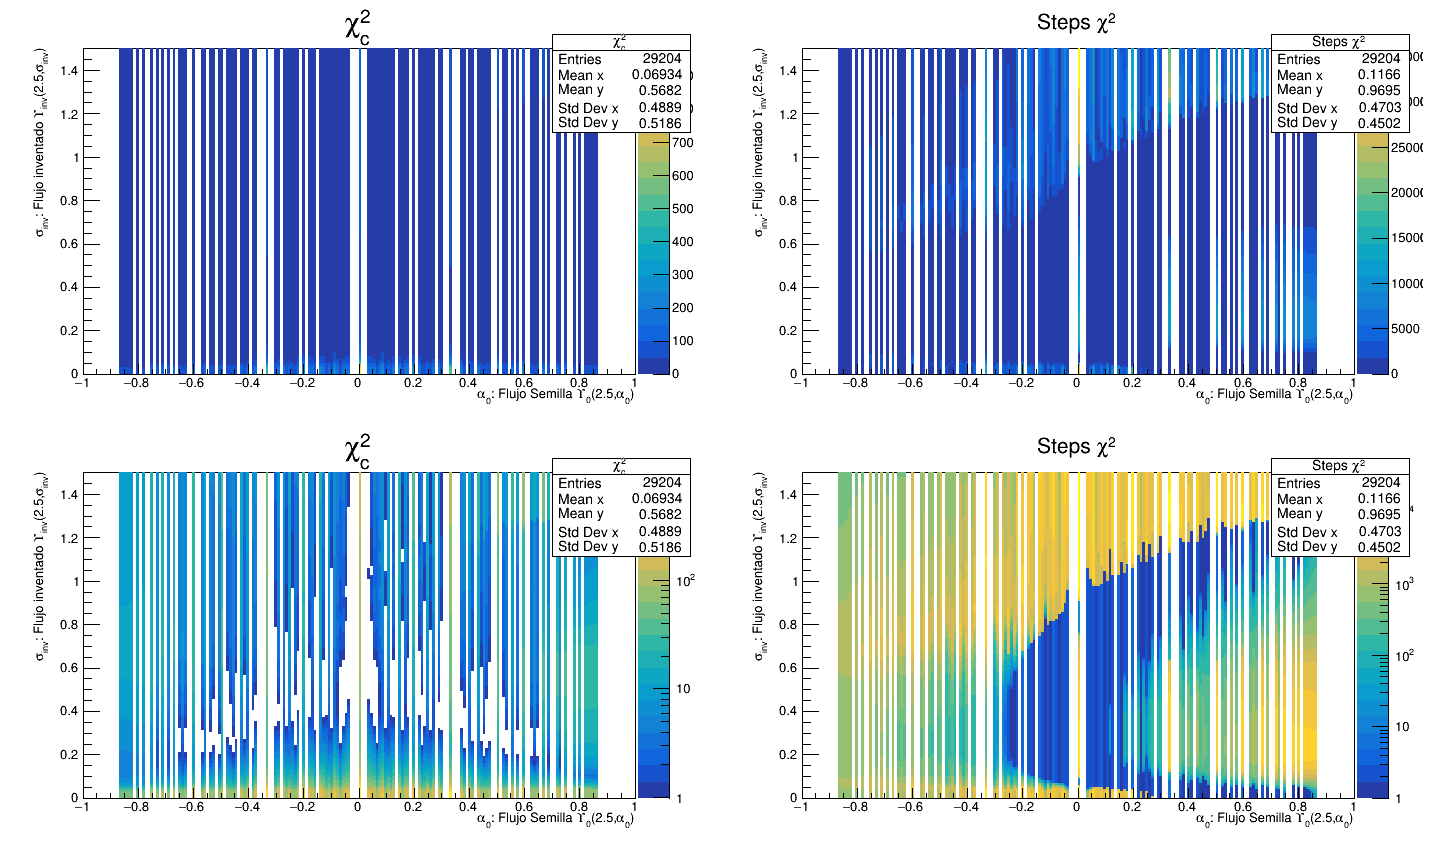
\includegraphics[width=1.\textwidth]{img/plot_deconv_21_fail_01.png}
    \centering
     \cprotect\caption{Grafico salida de la función \verb|neutrones_deconv_plot_21().|} 
\label{neutrones_deconv_plot_21_fail}
\end{figure}

Del gráfico (\ref{neutrones_deconv_plot_21_fail}) vemos claramente que hay un problema con el bineado en el eje horizontal. Es por esto que aparecen líneas en blanco en ese eje. El bineado es establecido al crear los histogramas \verb|TH2F| en la macro  \verb|deconvoluciones.C| de la siguiente manera:

\begin{lstlisting}[language=c++]
...
TH2F *hcol1 = new TH2F("#chi_{c}^{2}","#chi_{c}^{2}",196,-1.0,1.0,149,0,1.5);
TH2F *hcol2 = new TH2F("Steps #chi^{2}","Steps #chi^{2}",196,-1.0,1.0,149,0,1.5);
..
\end{lstlisting}

En los dos histogramas anteriores, al establecer para el eje vertical el bineado como \verb|..,149,0,1.5)| estamos diciendo que los anchos de los bines corresponden a anchos fijos de valor $(1.5-0)/149 = 0.010067114$. Y en el eje horizontal establecemos un bineado de ancho fijo de valor $|-1.0-1.0|/196=0.010204082$. Sin embargo. para este último, dados los datos, se tiene que los anchos de los bines deberían de ser variables, ya que el valor de $\alpha$ es oscilante.

Notemos que en el gráfico al cambiar ligeramente el bineado del eje vertical, por el siguiente:

\begin{lstlisting}[language=c++]
...
TH2F *hcol1 = new TH2F("#chi_{c}^{2}","#chi_{c}^{2}",196,-1.0,1.0,150,0,1.5);
TH2F *hcol2 = new TH2F("Steps #chi^{2}","Steps #chi^{2}",196,-1.0,1.0,150,0,1.5);
..
\end{lstlisting}

 es decir, a un ancho fijo de 0.01, el cual corresponde al paso exacto de los valores de la variable $\sigma_{inv}$ (que va desde 0.01 hasta 1.49) se obtiene lo siguiente:
 
 \begin{figure}[H]
    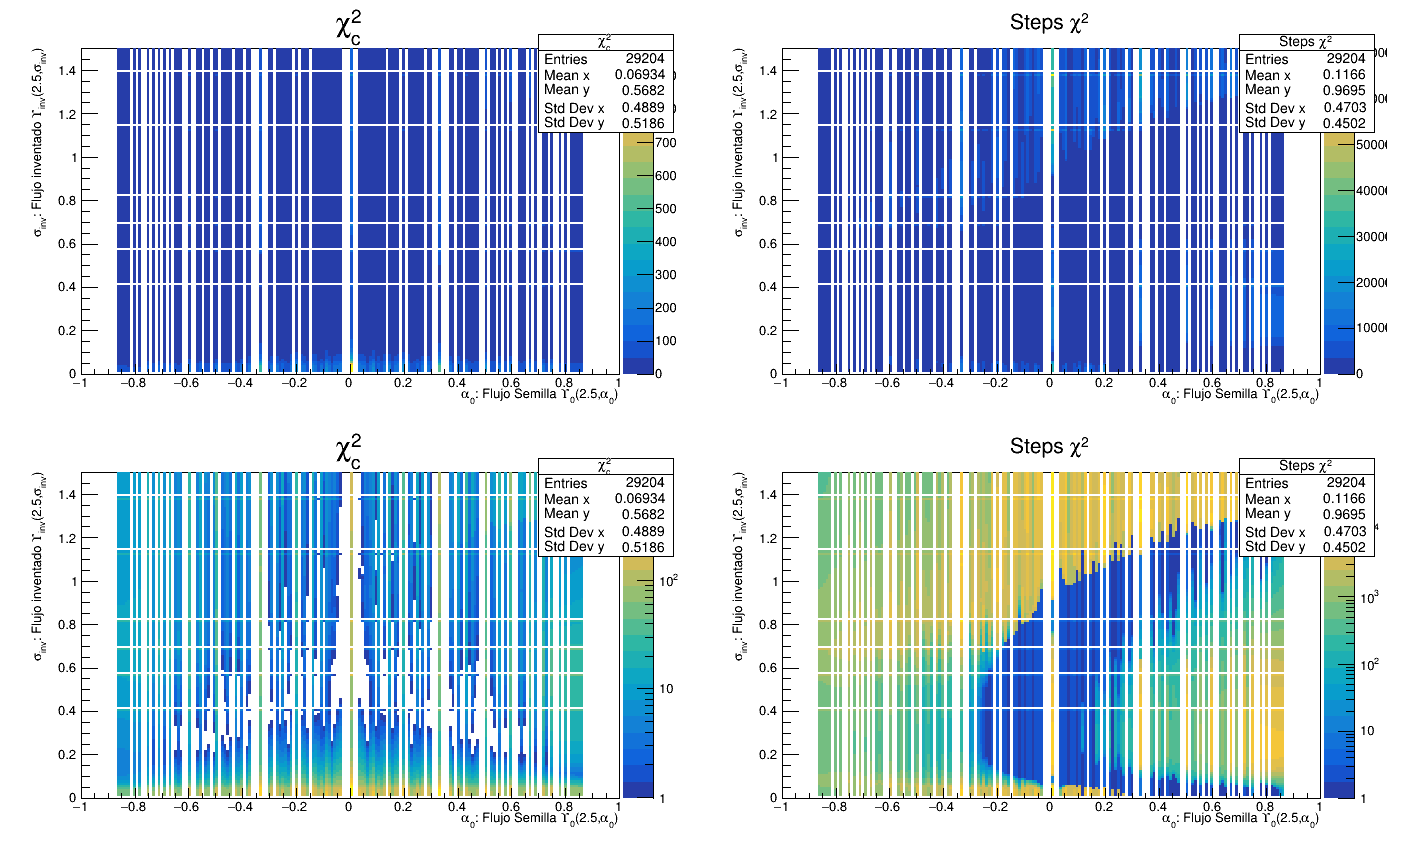
\includegraphics[width=1.\textwidth]{img/plot_deconv_21_fail_02.png}
    \centering
     \cprotect\caption{Grafico salida de la función \verb|neutrones_deconv_plot_21().|} 
\label{neutrones_deconv_plot_21_fail_02}
\end{figure}

Donde obtenemos líneas blancas horizontales, lo cual indica un bineado incorrecto(?) en el eje vertical.

Luego, haciendo distintas pruebas con el bineado del eje vertical, notamos que anchos fijos de bin de valores 0.01 ejem: (151,0,1.51), (149,0,1.49), generan líneas blancas horizontales. Mientras que bineados de anchos con mayores decimales: 0.010068493 ejem: (146,0,1.47) no generan líneas blancas.

El valor de $\alpha$ al que llamamos \textit{skewness}, u factor de oblicuidad o deformación de la distribución, lo calculamos de la siguiente manera:

\begin{align}
\alpha = \frac{\sigma_R-\sigma_L}{\sigma_R+\sigma_L}
\label{alpha_cust}
\end{align}

donde $\sigma_R$ y $\sigma_L$ corresponden a los anchos derecho e izquierdo de las distribuciones gaussianas usadas para construir una distribución semilla asimétrica. $\alpha$ así definida toma valores pertenecientes al intervalo $]-1,1[$, que para valores negativos me indica que la distribución tiene una inclinación hacia la izquierda y para valores positivos, tiene una inclinación hacia la derecha.

Sin embargo, notamos que al hacer un \verb|SetMaximun()| en el pad1 aparece un valor de 983.307, lo cuál es incorrecto para el valor de $\chi^2$, ya que de acuerdo al archivo \verb|chi2_test.dat| el valor máximo de $\chi^2$ no es mayor a 100. De esta manera, el valor incorrecto mencionado, se debe a que estamos asignando para un mismo valor de coordenadas $(\alpha,\sigma_{inv})$ en el mapa de calor, distintos valores de $\chi^2$, luego estos se van sumando en el eje $z$.

Para comprobar esto, definimos la función \verb|neutrones_deconv_plot_21_debug()| en la macro \verb|deconvoluciones.C|. Esta función genera un archivo de nombre \verb|objets_debug_test.dat| en el cual además de imprimir todos los parámetros de la simulación 21, se muestra también en la última columna el valor de skewness ($\alpha$). \newline
Lo que haremos ahora será cambiar la salida al archivo \verb|objets_debug_test.dat| para que el par $(\alpha,\sigma_{inv})$ sean las columnas finales y así mediante las herramientas del procesador de texto \verb|geany| buscar las repeticiones de pares ordenados. Así, encontramos lo siguiente:

\begin{itemize}
\item[•] 4 repeticiones del par $(0.5, 0.01)$, donde la suma de los $\chi^2$ es 293.72.
\item[•] 14 repeticones del par $(0,0.04)$ donde la suma de los $\chi^2$ es 811.29807.
\end{itemize}

Y así sucesivamente, lo cuál está dentro del orden del valor máximo de $\chi^2$ encontrado con  \verb|SetMaximun()|.

Este problema queda de manifiesto también al graficar el ancho izquierdo y derecha de la distribución gaussiana asimétrica de la semilla como mapa de calor, donde el eje z corresponde al valor de $\alpha$ (ver Fig. \ref{neutrones_deconv_plot_21_debug}):

\begin{figure}[H]
    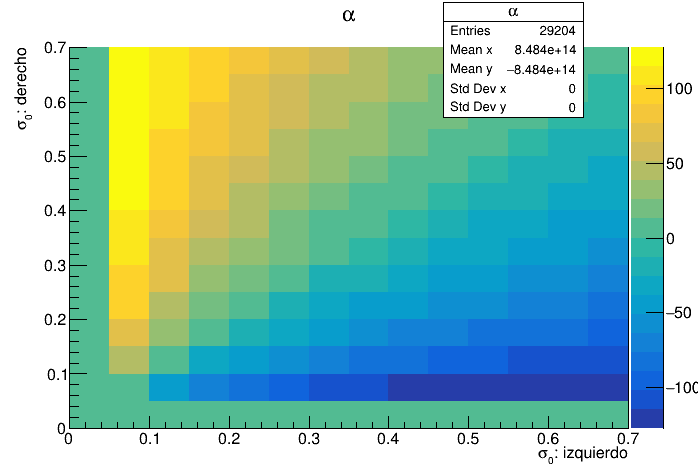
\includegraphics[width=0.8\textwidth]{img/sigma_izq_vs_der_alphaz.png}
    \centering
     \cprotect\caption{Grafico salida de la función \verb|neutrones_deconv_plot_21_debug().|} 
\label{neutrones_deconv_plot_21_debug}
\end{figure}

donde el máximo valor de $\alpha$ corresponde a $127.714$ y el mínimo corresponde a -127.714, lo cuál contradice la definición dada de $\alpha$, ya que sus valores deben oscilar entre -1 y 1, manifestando entonces que hay una repetición de pares $\sigma$ izquierdo y derecho (de manera que el valor de $\alpha$ se va sumando). Esto se puede ver al utilizar la herramienta de Find Document Usage en geany, mostrando por ejemplo que el par $(0.05,0.05)$ se repite al menos 100 veces en \verb|objets_debug_test.dat|.

\subsection*{Simulación 22}

Instrucciones para su ejecución:

\begin{itemize}
\item \verb|ulimit -n 39000|: donde 38416 es el número total de filas en \verb|chi2_test_deconv_22.dat|
\item \verb|root -l|
\item \verb|.L InitVar.cc++|
\item \verb|.L ANPulses.cc++|
\item \verb|.L neutron_sim_generator.C|
\item \verb|neutron_sim_generator_merge_fluxinvAG()|: Se genera el archivo \verb|neutrones_calculados_merge.dat| con los neutrones calculados asociados a un disparo (ancho determinado) y sistema de detección. Los pasos de ancho para el flujo corresponden a 0.05 o 50 keV, tanto como para el ancho izquierdo y derecho. Así, fijamos primero el ancho izquierdo en 0.05 y el ancho derecho aumenta en pasos de 0.05 comenzando desde 0.05 hasta el valor máximo de 0.7. Una vez logrado este valor para el ancho derecho, aumentamos el ancho izquierdo en 0.05 e iniciamos nuevamente con la variación del ancho derecho. La iteración termina cuando ambos anchos logren el máximo de 0.7 
\item \verb|.L deconvoluciones.C|
\item \verb|neutrones_deconv_22()|: 
Función que realiza las deconvoluciones utilizando semillas gaussianas asimétricas (2) y flujos inventados gaussianos asimétricos (2). En ambas distribuciones los pasos de energía para las iteraciones pueden ser ajustados. Se usaron pasos de 0.05 o 50 keV para las anchos izquierdo y derecho de los flujos semilla asimétricos (como máximo 0.7 por cada lado). Se genera entonces el archivo \verb|chi2_test.dat| donde los datos de las columnas corresponden a (visto como vector en c++) a lo mostrado en la entrada del \ref{2021-12-23}.

Input: \verb|neutrones_calculados_merge.dat| Output:  \verb|chi2_test.dat|.
\end{itemize}

De esta manera, el gráfico generado es el siguiente:

 \begin{figure}[H]
    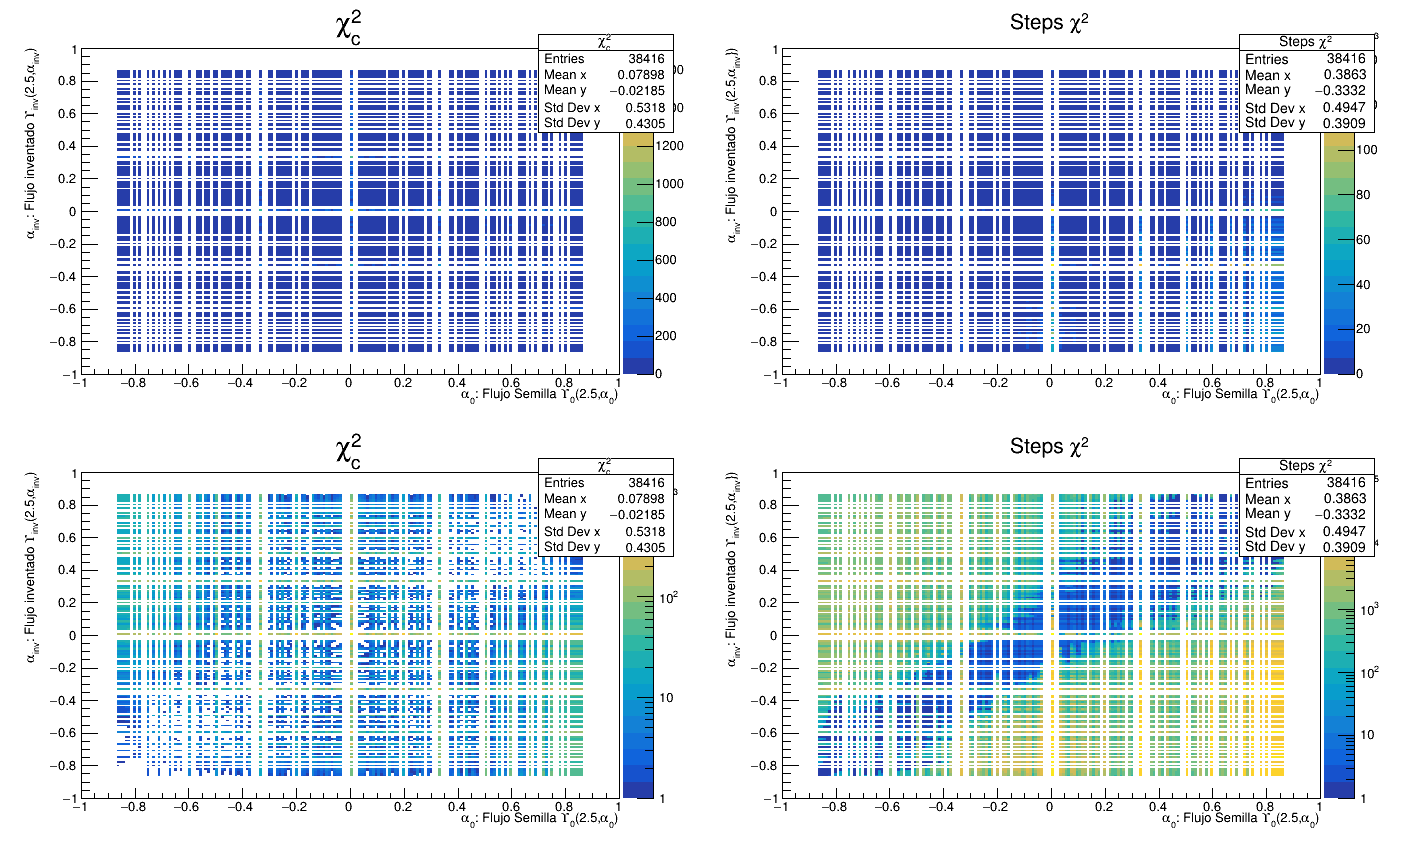
\includegraphics[width=1.\textwidth]{img/plot_deconv_22_fail.png}
    \centering
     \cprotect\caption{Grafico salida de la función \verb|neutrones_deconv_plot_22().|} 
\label{neutrones_deconv_plot_22_fail}
\end{figure}

Notamos nuevamente en la  Fig. \ref{neutrones_deconv_plot_22_fail} un error en el bineado tanto en el eje vertical como horizontal. Además, al hacer un \verb|SetMaximum| en el pad11 obtenemos un valor de $\chi^2$ igual a 1714.14, el cual es incorrecto, ya que este no debería superar el valor 100. Esto se debe a un problema idéntico al de la simulación 21, es decir, tenemos pares $(\alpha_{0},\alpha_{inv})$ repetidos, por lo que se van sumando los valores de $\chi^2$.

Las salidas de las deconvoluciones de las simulaciones 21 y 22 serán renombradas respectivamente como:

\begin{itemize}
\item \verb|chi_test_deconv_21_fail.dat|
\item  \verb|chi_test_deconv_22_fail.dat| 
\end{itemize}

\section{Entrada del 2022-01-11}
\label{2022-01-11}


Para solucionar el problema debido al uso de la definición propia de $\alpha$ dada en la ecuación \eqref{alpha_cust}. Utilizaremos la definición de $\alpha$ dada por el conjunto de librerías de \verb|c++| de nombre \verb|boost| (\url{https://www.boost.org/}), para esto instalamos la version 1.71.0 de \verb|libboost-all| para Ubuntu. En específico, usaremos el set de herramientas (toolkit) \verb|math| (\url{https://www.boost.org/doc/libs/1_71_0/libs/math/doc/html/index.html}) de \verb|boost|, en su versión 2.10.0. Dentro la librería \verb|math| en la sección \verb|distribuitons| usaremos la llamada \textbf{Skew Normal Distribution} (\url{https://www.boost.org/doc/libs/1_71_0/libs/math/doc/html/math_toolkit/dist_ref/dists/skew_normal_dist.html}).

Luego, guiados por el ejemplo en stackoverflow (\url{https://stackoverflow.com/questions/43450880/using-boost-skew-normal-distribution}) creamos una macro de \verb|root| de nombre \verb|skew_normal.C| donde haremos pruebas de la distribución  \textit{skew normal} de \verb|boost|. En esta macro definimos la función \verb|skew()| como un objeto tipo puntero \verb|TF1|, la cual toma como parámetro un \verb|double| de nombre \verb|alpha| que es el valor de la oblicuidad o skewness que tendrá la distribución que definiremos dentro de la función:

\begin{lstlisting}[language=c++]
#include <boost/math/distributions/skew_normal.hpp>
...
using namespace boost::math;
using namespace std;

TF1* skew(double_t alpha){

...

}
...
\end{lstlisting}

Luego, dentro de \verb|skew()| en las primeras líneas convertimos la variable \verb|alpha| en una tipo \verb|string|, para poder imprimirla como título en un gráfico de la distribución:

\begin{lstlisting}[language=c++]
...
	// Create an output string stream
	std::ostringstream stream_alpha;
	std::ostringstream stream_skewness;
	// Set Fixed -Point Notation
	stream_alpha << std::fixed;
	stream_skewness << std::fixed;
	
	// Set precision to 1 digits
	stream_alpha << std::setprecision(1);
	stream_skewness << std::setprecision(3);
	//Add double to stream
	stream_alpha << alpha;
	
	// Get string from output string stream
	std::string alpha_shape = stream_alpha.str();
...
\end{lstlisting}

Luego hacemos uso de la función \verb|skew_normal()| y la transformamos a una pdf vía la función \verb|pdf()|, ambas de la librería \verb|math| de \verb|boost| (\verb|boost::math::function()|), y a partir de esta creamos el objeto \verb|TF1| (función en 1-D) como puntero, de nombre \verb|skewNormal|:

\begin{lstlisting}[language=c++]
TF1 *skewNormal = new TF1("skewNormal", "pdf(skew_normal([0], [1], [2]), x)",0,7);
\end{lstlisting}\label{skew_normal_code_def}


La distribución skew normal es una variante de la bien conocida distribución normal o distribución de gauss. De hecho una distribución skew normal con el parámetro de forma o \textit{shape} igual a cero corresponde a la distribución normal, por lo que esta última puede ser considerada un caso especial de la más genérica distribución skew normal.

Sabemos que la distribución normal es de la forma:

\begin{align}
{\displaystyle \varphi(x)={\frac {1}{\sigma {\sqrt {2\pi }}}}e^{-{\frac {1}{2}}\left({\frac {x-\mu }{\sigma }}\right)^{2}}}
\end{align}

luego considerando los valores de los parámetros \textit{mean}: $\mu =0 $ y la desviación estándar o \textit{scale}: $\sigma=1$, entonces la distribución queda como 

\begin{align}
{\displaystyle \varphi(x)={\frac {1}{{\sqrt {2\pi }}}}e^{-\frac{x^2}{2}}}
\end{align}

Ahora, calculamos la función de distribución acumulada o cumulative distribution function (CDF):

\begin{align}
\Phi (x)=\int _{{-\infty }}^{{x}}\varphi (t)\ dt={\frac  {1}{2}}\left[1+\operatorname {erf}\left({\frac  {x}{{\sqrt  {2}}}}\right)\right]
\end{align}

Entonces, la función de densidad de probabilidad o probability density function (PDF) de la distribución skew normal con parámetro de shape $\alpha$ corresponde a:

\begin{align}
f(x)=2\varphi (x)\Phi (\alpha x),
\end{align}

Ahora, necesitamos agregar los parámetros \textit{location} ($\xi$) y \textit{shape} ($\omega$), para esto realizamos el siguiente cambio de variable a la función $f(x)$:

\begin{align}
x\rightarrow {\frac  {x-\xi }{\omega }}
\end{align}

resultando:

\begin{align}
f(x) &= \frac{1}{\omega}\frac{1}{\sqrt{2\pi}}e^{-\frac{1}{2}\left( \frac{x-\xi }{\omega }\right)^{2}} \int_{{-\infty }}^{\left(\alpha \left(\frac{x-\xi }{\omega } \right)\right)}\frac{1}{\sqrt{2\pi}}e^{-\frac{t^2}{2}}\ dt \nonumber \\
f(x) &= \frac{1}{(\omega \pi)}e^{-\frac{1}{2}\left( \frac{x-\xi }{\omega }\right)^{2}} \int_{{-\infty }}^{\left(\alpha \left(\frac{x-\xi }{\omega } \right)\right)}e^{-\frac{t^2}{2}}\ dt
\label{skew_normal_dist_mathdef}
\end{align}

Se puede verificar que la distribución normal se recupera cuando ${\displaystyle \alpha =0}$, y que el valor absoluto de la asimetría aumenta a medida que aumenta el valor absoluto de ${\displaystyle \alpha }$. La distribución está sesgada a la derecha si ${\displaystyle \alpha >0}$ y está sesgada a la izquierda si ${\displaystyle \alpha <0}$.

Esta definición \eqref{skew_normal_dist_mathdef} es utilizada en la línea de código \eqref{skew_normal_code_def} que escribimos anteriormente, donde los parámetros de la distribución skew normal tienen que ser establecidos:

\begin{itemize}
\item location ($\xi$): $[0]$
\item scale ($\omega$): $[1]$
\item shape ($\alpha$): $[2]$
\end{itemize}


De la definición de \verb|skew_normal_distribution| en \verb|boost| tenemos que \textit{location}, \textit{scale} y \textit{shape} corresponden a:


\begin{lstlisting}[language=c++]
// Constructor:
  skew_normal_distribution(RealType location = 0, RealType scale = 1, RealType shape = 0);
   // Accessors:
   RealType location()const; // mean if normal.
   RealType scale()const; // width, standard deviation if normal.
   RealType shape()const; // The distribution is right skewed if shape > 0 and is left skewed if shape < 0.
                          // The distribution is normal if shape is zero.
\end{lstlisting}

Siguiendo con la función \verb|TF1| definido anteriormente, seteamos los valores antes nombrados:

\begin{lstlisting}[language=c++]
...
skewNormal->SetParameters(2.5,1,alpha);
...
\end{lstlisting}

Luego para obtener el valor de skewness o $\gamma_1$, utilizaremos la función \verb|boost::math::skewness()|, de la siguiente manera:

\begin{lstlisting}[language=c++]
cout<< skewness(skew_normal_distribution<double>(2.5,1.,alpha)) << endl;

    /*Valor de la oblicuidad */
	double_t sk = skewness(skew_normal_distribution<double>(2.5,1.,alpha));

	stream_skewness << sk;
	std::string boost_skewness = stream_skewness.str();
	
	
	//~ skewNormal->SetTitle(alpha_shape.c_str());
	skewNormal->SetTitle(boost_skewness.c_str());
\end{lstlisting}

Finalmente, la función \verb|skew()| regresa una función de root tipo \verb|TF1| definida como una distribución skew normal con los siguientes parámetros:

\begin{itemize}
\item location ($\xi$): $[0]=2.5$
\item scale ($\omega$): $[1]=1$
\item shape ($\alpha$): $[2]=$ \verb|alpha|
\end{itemize}

Luego utilizamos esta función (\verb|skew()|) para generar un canvas con 16 distribuciones skew normal (ver Fig. \ref{skew_normal_dist}) para distintos valores del parámetro shape ($\alpha$), y por lo tanto, distintos valores de skewness ($\gamma_1$). Ambos parámetros mostrados en el título de cada pad junto con el valor de location y scale de cada distribución:

 \begin{figure}[H]
    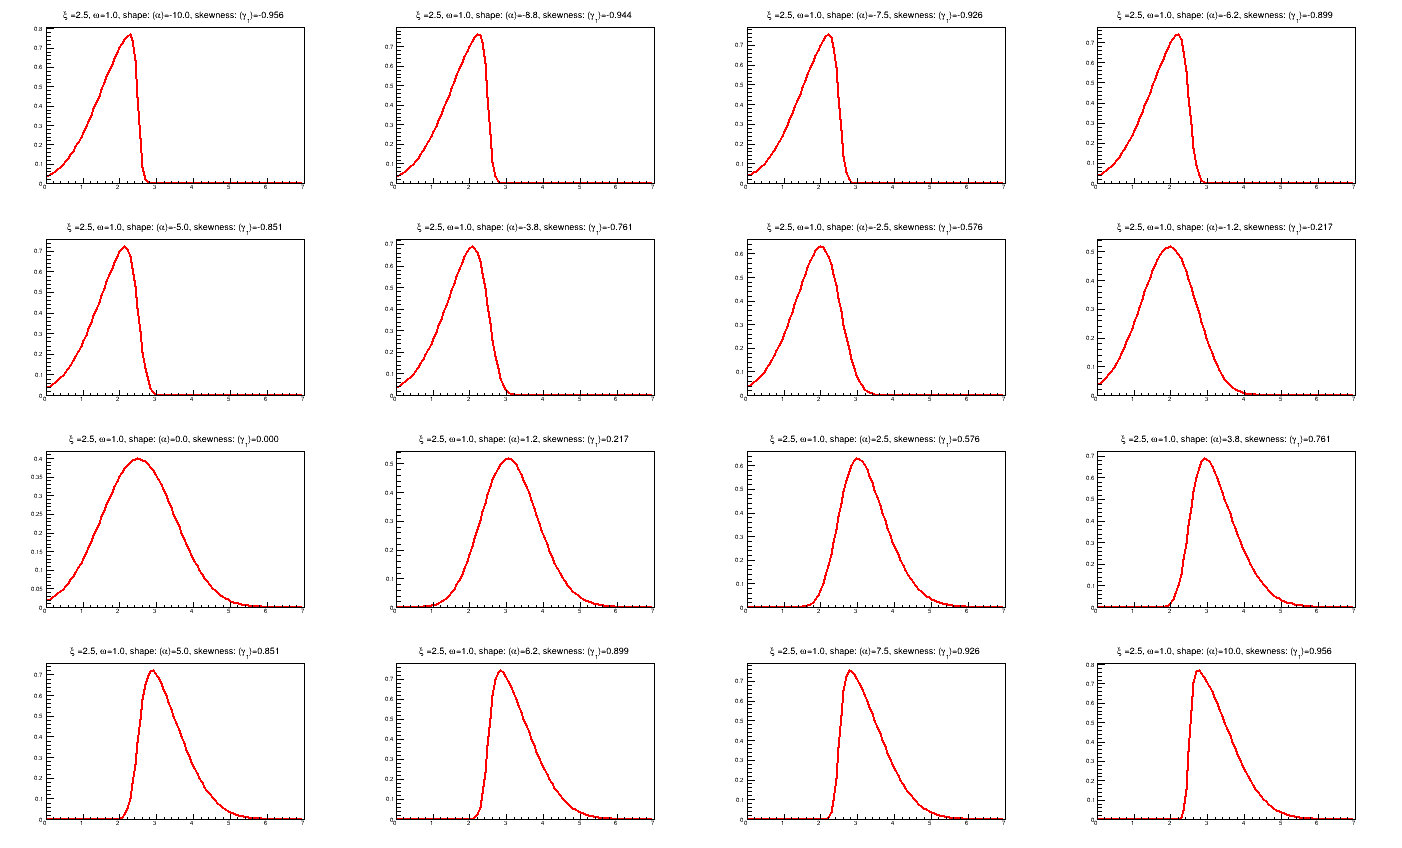
\includegraphics[width=1.\textwidth]{img/skew_normal_dist.png}
    \centering
     \cprotect\caption{Grafico salida de la macro \verb|skew_normal.C|} 
\label{skew_normal_dist}
\end{figure}



También generamos otro canvas con las 16 distribuciones superpuestas en un solo gráfico:

 \begin{figure}[H]
    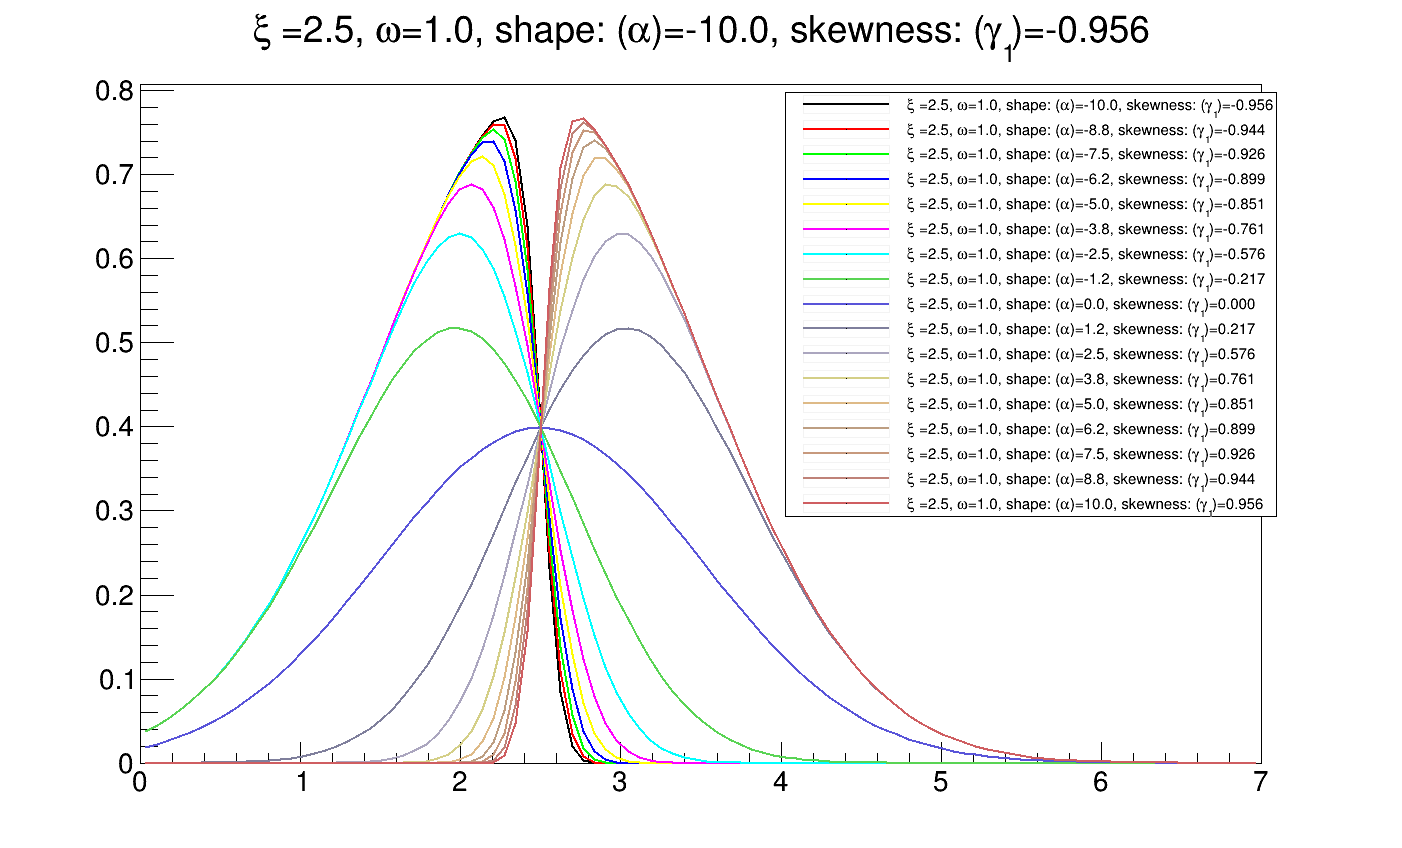
\includegraphics[width=1.\textwidth]{img/skew_normal_dist_same.png}
    \centering
     \cprotect\caption{Grafico salida de la macro \verb|skew_normal.C| con las 16 distribuciones en un solo gráfico. En el título se muestran los parámetros de la distribución de mayor amplitud de la izquierda.} 
\label{skew_normal_dist_same}
\end{figure}

De la Fig. \ref{skew_normal_dist_same} notamos que el valor del skewness de la distribución varía de izquierda a derecha desde el valor $\gamma_1=-0.956$ pasando por $\gamma_1=0$ que es cuando la distribución corresponde a una distribución normal de promedio 2.5 y de desviación estándar igual a 1, hasta llegar al valor máximo de $\gamma_1=0.956$. En esta evolución el valor de la \textit{moda} de la distribución (ver Fig.
\ref{skew_normal_dist_parameters}) es distinto para cada distribución. Entonces, si queremos hacer uso de estas en las deconvoluciones, tienen que tener la misma \textit{moda} y \textit{altura} pero distinto valor de skewness, ya que se quiere estudiar el efecto en las deconvoluciones al mover un solo parámetro a la vez en la semilla.

 \begin{figure}[H]
    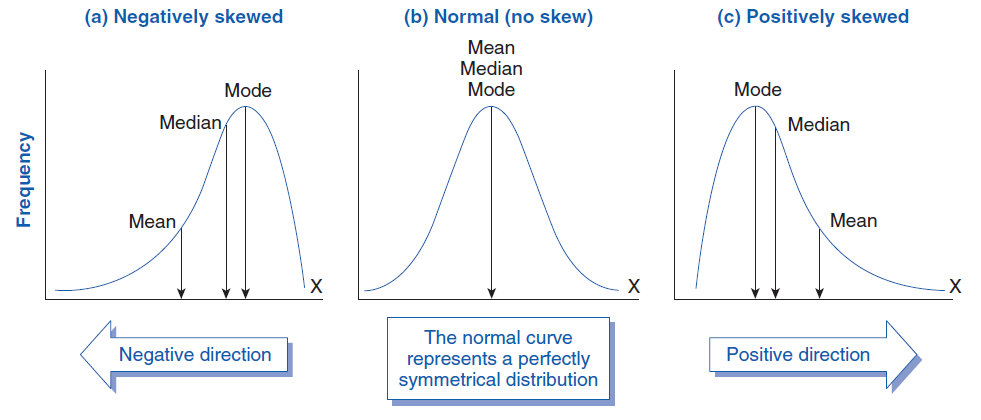
\includegraphics[width=1.\textwidth]{img/skew_normal_parameters.png}
    \centering
     \cprotect\caption{Caracterización de un distribución skew normal. Fuente: \url{https://www.biologyforlife.com/skew.html} } 
\label{skew_normal_dist_parameters}
\end{figure}

De acuerdo a la librería \verb|math| de \verb|boost| tenemos varias funciones implementadas para la distribución skew normal, de las cuales seleccionamos las que nos servirán para nuestro código, y que son mostradas a continuación:


\begin{table}[H]
\centering
\begin{tabular}{|c|c|}
\hline
\textbf{Function} & \textbf{	
Implementation Notes} \\
\hline
pdf & Usando: $f(x) = \frac{1}{(\omega \pi)}e^{-\frac{1}{2}\left( \frac{x-\xi }{\omega }\right)^{2}} \int_{{-\infty }}^{\left(\alpha \left(\frac{x-\xi }{\omega } \right)\right)}e^{-\frac{t^2}{2}}\ dt$ \\
\hline
location & $\xi$ \\
\hline
scale &  $\omega$ \\
\hline
shape & $\alpha$ \\
\hline
quantile & Maximum of the pdf is sought through searching the root of $f'(x)=0$ \\
\hline
median & quantile(1/2) \\
\hline
mean & $\xi + \omega \delta \sqrt{\frac{2}{\pi}}$ donde $\delta = \frac{\alpha}{\sqrt{(1+\alpha^2)}}$ \\
\hline
mode & Maximum of the pdf is sought through searching the root of $f'(x)=0$ \\
\hline
variance & $\omega^2\left( 1-2\frac{\delta^2}{\pi}\right)$ \\
\hline
skewness & $  \gamma_1 = \frac{(4-\pi)}{2} \frac{\left(\delta \sqrt{\frac{2}{\pi}} \right)^3}{\left(1-2\frac{\delta^2}{\pi} \right)^{3/2}}$ \\
\hline
\end{tabular}
\caption{Nombre de las funciones y su implementación en la librería math para distribuciones skew normal}
\label{boost_functions}
\end{table}

Entonces, si queremos generar distintas distribuciones semilla o inventadas con valores de skewness distintos, se tiene que elegir un conjunto de $\alpha$'s que generen un conjunto de $\gamma_1$. Para esto, necesitamos como se comporta $\gamma_1$ en función de $\alpha$. Por lo que graficaremos $\gamma_1(\alpha)$ dada la relación matemática de la tabla \ref{boost_functions}:

\begin{align}
 \gamma_1(\alpha) = \frac{(4-\pi)}{2} \frac{\left( \frac{\sqrt{2}\alpha}{\sqrt{(1+\alpha^2)}\pi} \right)^3}{\left(1-\frac{2\alpha^2}{(1+\alpha^2)\pi}\right)^{3/2}}
\end{align}

Obteniendo:

 \begin{figure}[H]
    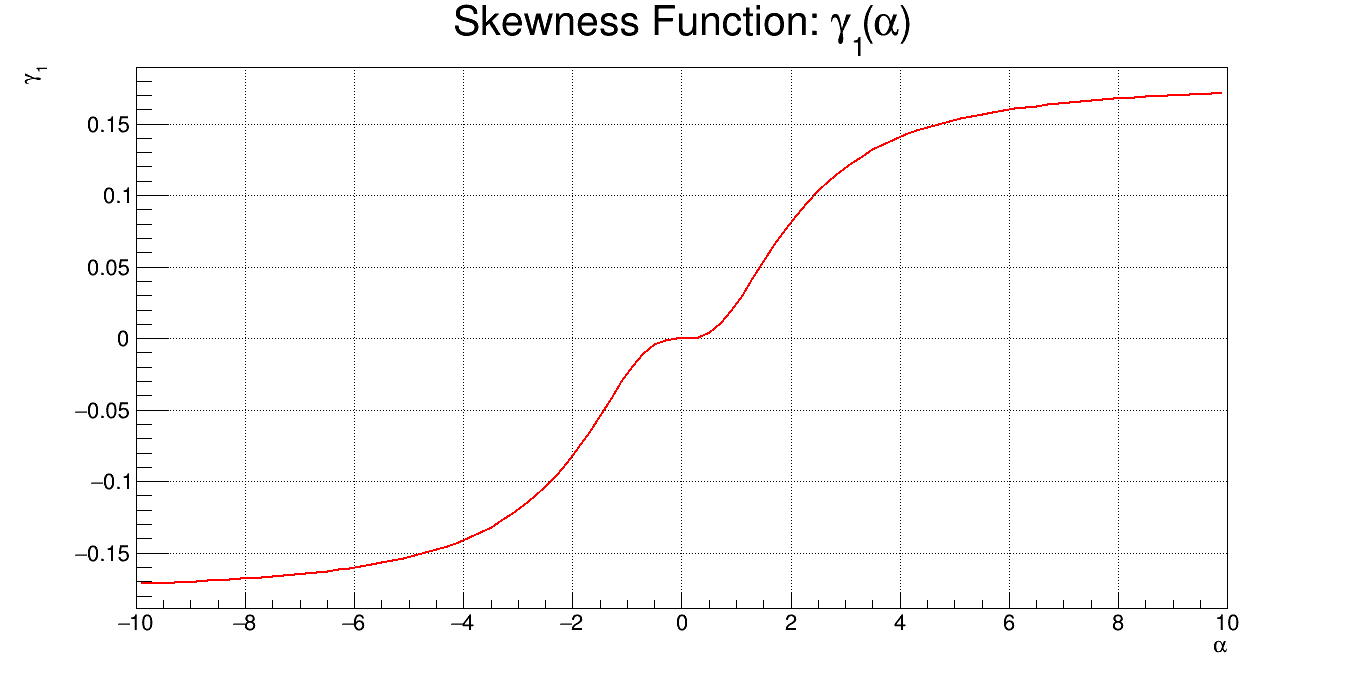
\includegraphics[width=1.\textwidth]{img/skewness_function.png}
    \centering
     \cprotect\caption{Gráfico de $\gamma_{1}(\alpha)$.} 
\label{skewness_function}
\end{figure}

En la vecindad de $\alpha=0$ la variación de $\gamma_1$ es pequeña. Luego desde $\alpha=0.5$ la función crece (y decrece) de manera rápida tipo logaritmo, hasta lograr un valor permanente cercano a 1 y -1 respectivamente.

\section{Entrada del 2022-01-13}

Luego de haber explorado las distribuciones skew normal definidas con la librería \verb|math| de \verb|boost|, las utilizaremos para repetir las simulaciones 21 y 22, con variaciones de $\gamma_{0}$ que se correspondan con un solo valor de $\sigma_{inv}$ y variaciones de $\gamma_{0}$ que se correspondan con un solo valor de $\gamma_{inv}$ respectivamente.

Se modificó la clase \verb|ANPulses.cc| en específico la función \verb|SeedGenerator()|, esto para incluir una nueva forma de definir una distribución asimétrica, usando el conjunto de librerías \verb|boost| (opción \verb|dist=3|). 

La inclusión se hace en las siguientes líneas de \verb|SeedGenerator()|:

\begin{lstlisting}[language=c++]
...
else if (dist==3)
	{
		/*Skew Normal Distribution*/
		double_t location = par1;
		double_t scale = 1.2;
		double_t shape = 1.0;

		for (int i = 0; i < binnum; i++)
		
			{
				content = 0;
		
				content = A*boost::math::pdf(boost::math::skew_normal(location, scale, SIG_L),bins[i]); //1.5
				seed[i] = content;
						
			}
		
	}
...
\end{lstlisting}

A continuación mostraremos los histogramas generadas con esta opción, usando la nueva función de la macro \verb|neutron_sim_generator.C|:
\begin{itemize}
\item[•] \verb|neutrones_sim_generator_merge_skewnormal_L_test()|
\end{itemize} 

 \begin{figure}[H]
    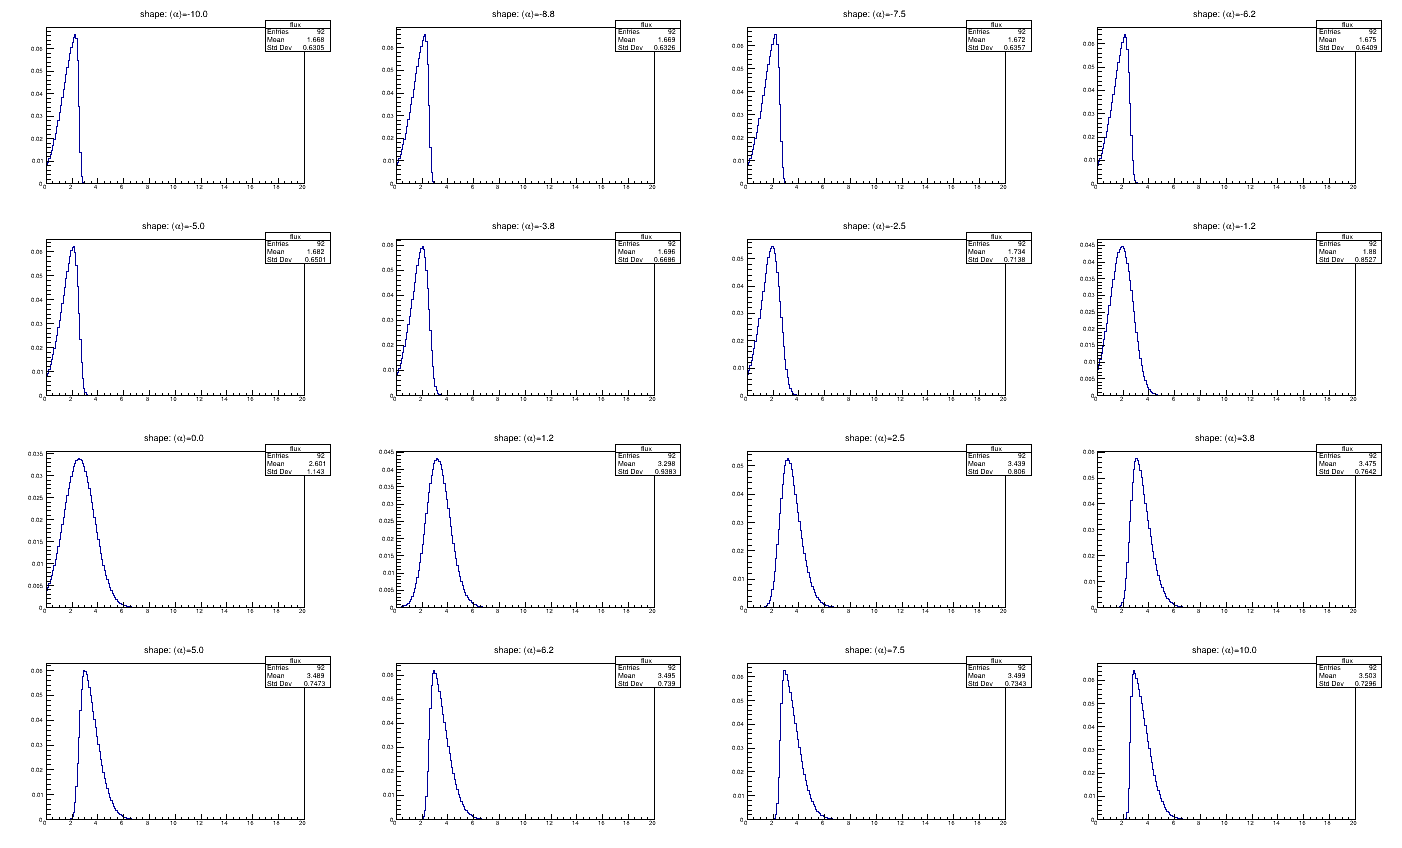
\includegraphics[width=1.\textwidth]{img/skew_normal_histogram_test_1.png}
    \centering
     \cprotect\caption{Histogramas de 16 distribuciones generados con \verb|SeedGenerator()| para la opción \verb|dist=3| en \verb|Test_Unfolding_TH1D(2.5,0.2,3,sigl1,1.0)|} 
\label{skew_normal_histogram_test_1}
\end{figure}

 \begin{figure}[H]
    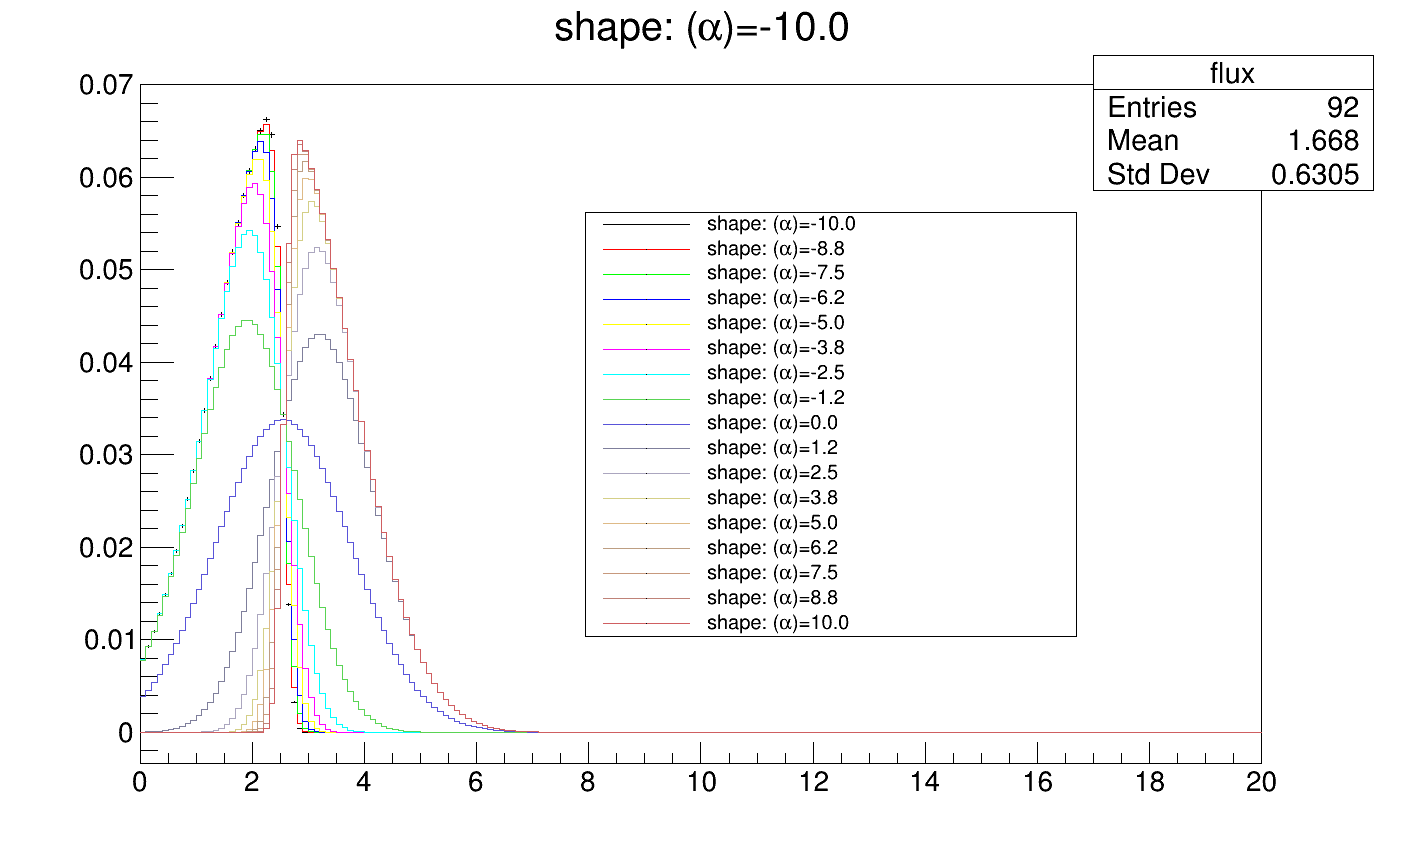
\includegraphics[width=1.\textwidth]{img/skew_normal_histogram_test_2.png}
    \centering
     \cprotect\caption{Superposición de histogramas de 16 distribuciones generados con \verb|SeedGenerator()| para la opción \verb|dist=3| en \verb|Test_Unfolding_TH1D(2.5,0.2,3,sigl1,1.0)|} 
\label{skew_normal_histogram_test_2}
\end{figure}

En la Fig \ref{skew_normal_histogram_test_1} al hacer click en cualquier caja de estadística y establecer la opción \verb|SetOptStat()| en 1001111, se puede ver que todos los histogramas están normalizados a 1, es decir, la integral de cada uno de estos es igual a 1.

En la Fig \ref{skew_normal_histogram_test_2} mostramos el valor del parámetro \textit{shape} para cada histograma. Notamos además que los histogramas del lado derecho tienen una amplitud ligeramente menor en comparación a sus  histogramas espejo del lado izquierdo. Pero estos deberían ser idénticos de acuerdo a la Fig \ref{skew_normal_dist_same}.

De esta manera, realizamos las siguientes simulaciones:

\subsection*{Simulacion 31 (usando boost)}

Instrucciones para su ejecución:

\begin{itemize}
\item \verb|ulimit -n 20000|: donde 18029  es el número total de filas en \verb|chi2_test.dat| (121 distribuciones semillas $\times$ 149 distribuciones gaussianas inventadas, es decir, por cada distribución inventada se itera (deconvoluciona) usando una semilla, generando un total de $121 \times 149=18029$ iteraciones.)
\item \verb|root -l|
\item \verb|.L InitVar.cc++|
\item \verb|.L ANPulses.cc++|
\item \verb|.L neutron_sim_generator.C|
\item \verb|neutron_sim_generator_merge_fluxinvG()|: Se genera el archivo \verb|neutrones_calculados_merge.dat| con los neutrones calculados asociados a un disparo (ancho determinado) y sistema de detección. Los pasos de ancho para el flujo corresponden a 0.01 o 10 keV, con un máximo de 1.49. Generando de esta manera 149 distribuciones
\item \verb|.L deconvoluciones.C|
\item \verb|neutrones_deconv_31_skewnormal()|: \\
Input: \verb|neutrones_calculados_merge.dat| Output:  \verb|chi2_test.dat|.

Función que realiza las deconvoluciones utilizando semillas skew normal distribution (3) y flujos inventados gaussianos simétricos (1). En ambas distribuciones los pasos de energía para las iteraciones pueden ser ajustados, para la primera se ajusta el parámetro \verb|shape| ($\alpha$) y para la segunda el ancho de la distribución $\sigma$.
 
Dada la forma del skewness (ver Fig \ref{skewness_function}), el parámetro $\alpha$ para las semillas se varía en cuatro intervalos:

\begin{itemize}
\item[•] 1er intervalo: $[-10,-5[$ con pasos de $0.5$
\item[•] 2do intervalo: $[-5,-0.09[$ con pasos de $0.1$
\item[•] 3er intervalo: $[0,5]$ con pasos de $0.1$
\item[•] 4to intervalo: $[5.5,10]$ con pasos de $0.5$
\end{itemize}

Esta elección, genera 121 valores de $\alpha$ uniformen te distribuidos en cada uno de los intervalos anteriores. Así como 121 distribuciones skew normal (semilla), y por lo tanto, 121 valores distintos de skewness (con valores idénticos pero negativos con respecto al punto espejo $\gamma_1 = 0$).

Se genera entonces el archivo \verb|chi2_test.dat| donde los datos de las columnas corresponden a la salida generada por estas líneas de código (ver \verb|Pretty_EMsimple_em1()| de la clase $\verb|ANPulses|$).

\begin{lstlisting}[language=c++]
...
else if ( (dist==3) && (dist_inv==1))
{
double_t sk = boost::math::skewness(boost::math::skew_normal_distribution<double>(2.5,1.2,SIG_L));
double_t mode = boost::math::mode(boost::math::skew_normal_distribution<double>(2.5,1.2,SIG_L));
double_t median = boost::math::median(boost::math::skew_normal_distribution<double>(2.5,1.2,SIG_L));
double_t mean = boost::math::mean(boost::math::skew_normal_distribution<double>(2.5,1.2,SIG_L));
double_t variance = boost::math::variance(boost::math::skew_normal_distribution<double>(2.5,1.2,SIG_L));

           chi2_test << left <<setw(5)<< setfill(' ') << shot << " "
         <<setw(5) << setfill(' ') << it << " "
         <<setw(5) << setfill(' ') << SIG_L  << " " /*shape*/        
         <<setw(5) << setfill(' ') << sk  << " " /*skewness de boost libray*/
         <<setw(5) << setfill(' ') << mode  << " "
         <<setw(5) << setfill(' ') << median  << " "
         <<setw(5) << setfill(' ') << mean  << " "
         <<setw(5) << setfill(' ') << variance << " "
         <<setw(5) << setfill(' ') << par2_inv  << " "
         <<setw(5) << setfill(' ') << chi2_em2 << endl;

}
...
\end{lstlisting}

\item \verb|neutrones_deconv_plot_31_tgraph()|: Input: \verb|chi2_test.dat| Output: Dos mapas de calor generados con root.

\end{itemize}

Los mapas de calor generados son los siguientes:

 \begin{figure}[H]
    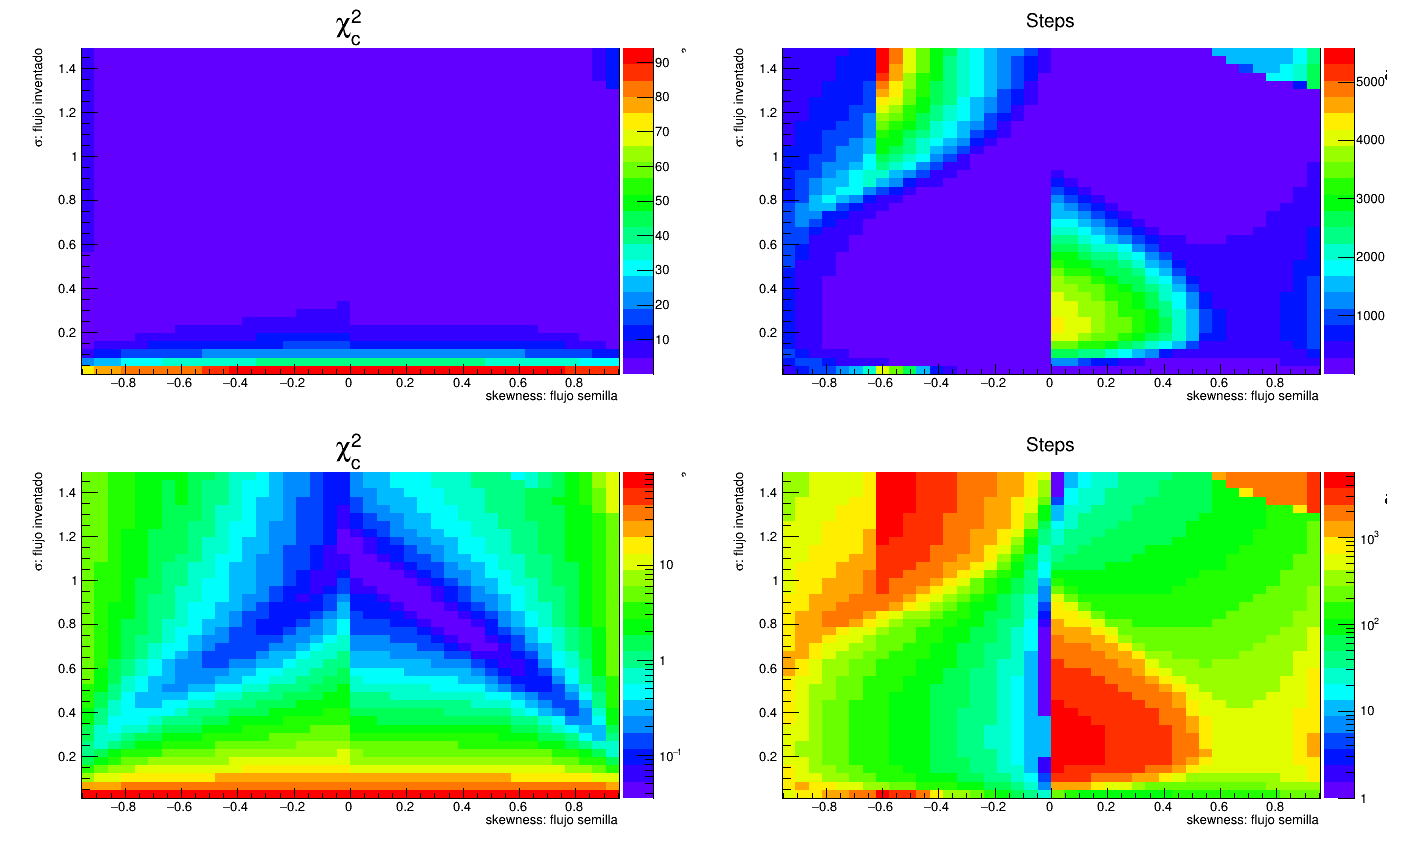
\includegraphics[width=1.\textwidth]{img/plot_deconv_31_tgraph_1.png}
    \centering
     \cprotect\caption{Grafico salida de la función \verb|neutrones_deconv_plot_31_tgraph()|. En los pad11 y 21 se grafica $\chi_c^2$ en función del valor del skewness del flujo semilla y el valor de $\sigma$ del flujo inventado.  En los pad12 y 22 se grafica los pasos que le toma converger a $\chi^2$  en función del valor del skewness del flujo semilla y el valor de $\sigma$ del flujo inventado.} 
\label{plot_deconv_31_tgraph_skewness}
\end{figure}

 \begin{figure}[H]
    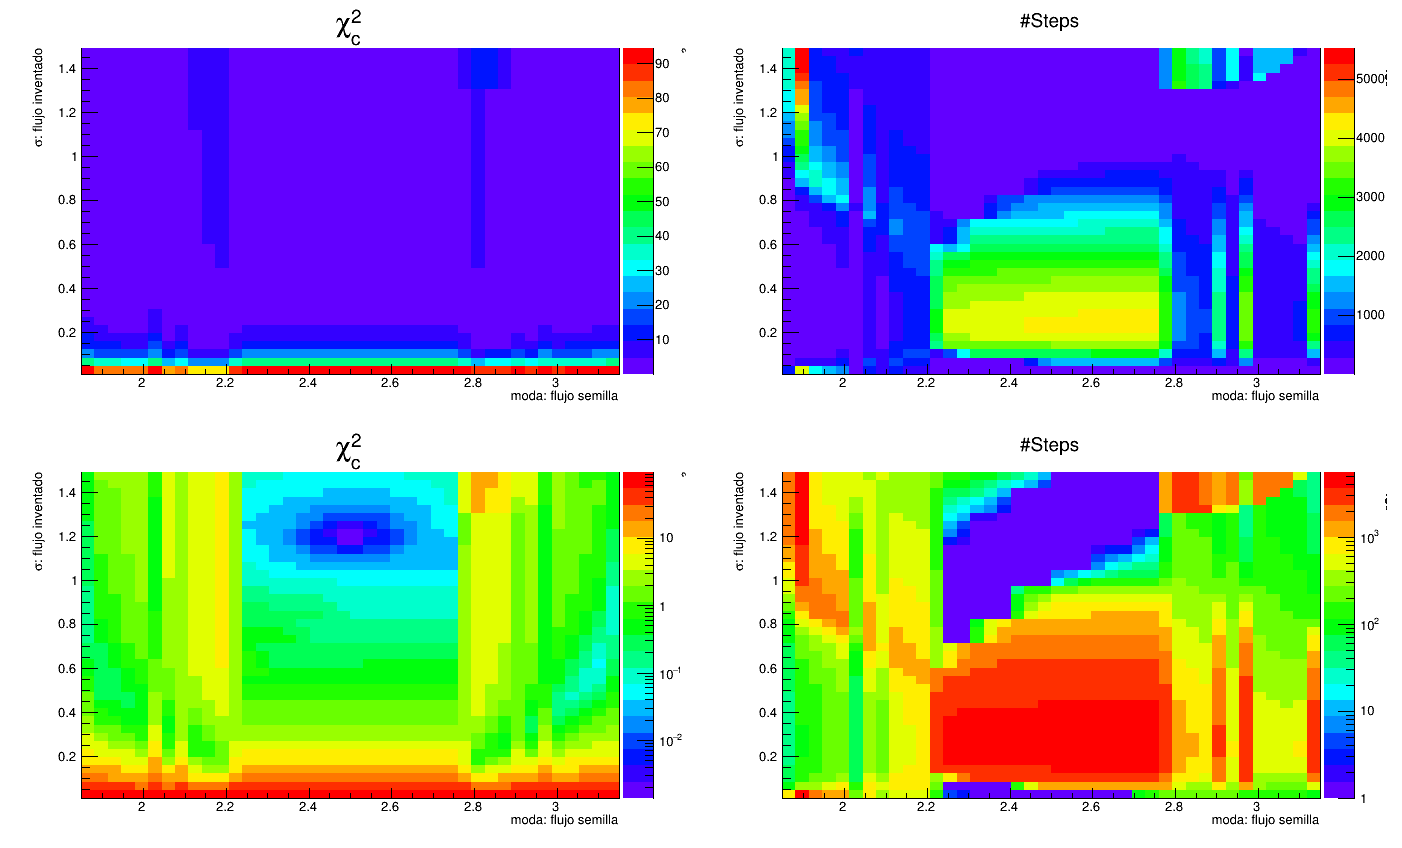
\includegraphics[width=1.\textwidth]{img/plot_deconv_31_tgraph_2.png}
    \centering
     \cprotect\caption{Grafico salida de la función \verb|neutrones_deconv_plot_31_tgraph()|. En los pad11 y 21 se grafica $\chi_c^2$ en función del valor de la moda del flujo semilla y el valor de $\sigma$ del flujo inventado.  En los pad12 y 22 se grafica los pasos que le toma converger a $\chi^2$  en función del valor de la moda del flujo semilla y el valor de $\sigma$ del flujo inventado.} 
\label{plot_deconv_31_tgraph_moda}
\end{figure}

El archivo de salida de salida de la simulación 31 de nombre \verb|chi2_test.dat| es renombrado como \verb|chi2_skewnormal_31_allst.dat|, donde en las distintas columnas y en orden ascendente se almacena 

\begin{itemize}
\item[•] \verb|shot|: número de disparo (asociado a un único parámetro $\sigma$ del flujo inventado)
\item[•] \verb|it|: pasos que le toma al algoritmo em1(\ref{EM1}) $\chi^2$ satisfacer su condición de salida o quiebre ($\chi^2>N$). 
\item[•] \verb|SIG_L|: Cuando en  \verb|Pretty_EMsimple_em1()| el valor de \verb|dist=3|, tenemos que el parámetro para la distribución semilla (\verb|SIG_L|) corresponde al shape ($\alpha$) de una distribución skew normal generada con boost de location $\xi=2.5$ y scale $\omega=1.2$. El parámetro \verb|SIG_R| no se considera en la salida ni tampoco para generar la distribución semilla.
\item[•] \verb|sk|: corresponde al skewness de la distribución semilla obtenida con \verb|boost|.
\item[•] \verb|mode|: corresponde a la moda de la distribución semilla obtenida con \verb|boost|.
\item[•] \verb|median|: corresponde a la mediana de la distribución semilla obtenida con \verb|boost|.
\item[•] \verb|mean|: corresponde al promedio de la distribución semilla obtenida con \verb|boost|.
\item[•] \verb|variance|: corresponde a la varianza de la distribución semilla obtenida con \verb|boost|.
\item[•] \verb|par2_inv|: corresponde al $\sigma$ de la distribución de flujo inventado.
\item[•] \verb|chi2_em2|: corresponde al valor de $\chi^2_c$ del algoritmo em2 \ref{EM2}, que resulta de comparar las formas del flujo deconvolucionado con el flujo inventado.
\end{itemize}


\subsection*{Simulacion 33 (usando boost)}

Instrucciones para su ejecución:

\begin{itemize}
\item \verb|ulimit -n 20000|: donde 18029  es el número total de filas en \verb|chi2_test.dat| (121 distribuciones semillas $\times$ 149 distribuciones gaussianas inventadas, es decir, por cada distribución inventada se itera (deconvoluciona) usando una semilla, generando un total de $121 \times 149=18029$ iteraciones.)
\item \verb|root -l|
\item \verb|.L InitVar.cc++|
\item \verb|.L ANPulses.cc++|
\item \verb|.L neutron_sim_generator.C|
\item \verb|neutrones_sim_generator_merge_skewnormal_L()|: \\
Se genera el archivo \verb|neutrones_calculados_merge.dat| con los neutrones calculados asociados a un disparo (valor de shape $\alpha$) y sistema de detección. Los pasos de $\alpha$ para el flujo corresponden a cuatro los dado en cuatro intervalos:

\begin{itemize}
\item[•] 1er intervalo: $[-10,-5[$ con pasos de $0.5$
\item[•] 2do intervalo: $[-5,-0.09[$ con pasos de $0.1$
\item[•] 3er intervalo: $[0,5]$ con pasos de $0.1$
\item[•] 4to intervalo: $[5.5,10]$ con pasos de $0.5$
\end{itemize}

Generando así 121 distribuciones skew normal como flujos inventados.

\item \verb|.L deconvoluciones.C|
\item \verb|neutrones_deconv_33_skewnormal()|: \\
Input: \verb|neutrones_calculados_merge.dat| Output:  \verb|chi2_test.dat|.
Función que realiza las deconvoluciones utilizando semillas skew normal distribution (3) y flujos inventados skew normal distribution (3). En ambas distribuciones los pasos de energía para las iteraciones pueden ser ajustados, siendo en las dos el parámetro \verb|shape| ($\alpha$). El cual se distribuye para las semillas de igual manera que para los flujos inventados que se mostró anteriormente.

\item \verb|neutrones_deconv_plot_33_tgraph()|: Input: \verb|chi2_test.dat| Output: Dos mapas de calor generados con root.

\end{itemize}



Se genera entonces el archivo \verb|chi2_test.dat| donde los datos de las columnas corresponden a la salida generada por estas líneas de código (ver \verb|Pretty_EMsimple_em1()| de la clase $\verb|ANPulses|$):

\begin{lstlisting}[language=c++]
else if ( (dist==3) && (dist_inv==3))
{
double_t sk = boost::math::skewness(boost::math::skew_normal_distribution<double>(2.5,1.2,SIG_L));
double_t mode = boost::math::mode(boost::math::skew_normal_distribution<double>(2.5,1.2,SIG_L));
double_t median = boost::math::median(boost::math::skew_normal_distribution<double>(2.5,1.2,SIG_L));
double_t mean = boost::math::mean(boost::math::skew_normal_distribution<double>(2.5,1.2,SIG_L));
double_t variance = boost::math::variance(boost::math::skew_normal_distribution<double>(2.5,1.2,SIG_L));

double_t sk_inv = boost::math::skewness(boost::math::skew_normal_distribution<double>(2.5,1.2,SIG_L_inv));
double_t mode_inv = boost::math::mode(boost::math::skew_normal_distribution<double>(2.5,1.2,SIG_L_inv));
double_t median_inv = boost::math::median(boost::math::skew_normal_distribution<double>(2.5,1.2,SIG_L_inv));
double_t mean_inv = boost::math::mean(boost::math::skew_normal_distribution<double>(2.5,1.2,SIG_L_inv));
double_t variance_inv = boost::math::variance(boost::math::skew_normal_distribution<double>(2.5,1.2,SIG_L_inv));

            chi2_test << left <<setw(5)<< setfill(' ') << shot << " "
         <<setw(5) << setfill(' ') << it << " "
         <<setw(5) << setfill(' ') << SIG_L  << " " /*shape semilla*/        
         <<setw(5) << setfill(' ') << sk  << " " /*skewness de boost libray*/
         <<setw(5) << setfill(' ') << mode  << " "
         <<setw(5) << setfill(' ') << median  << " "
         <<setw(5) << setfill(' ') << mean  << " "
         <<setw(5) << setfill(' ') << variance << " "
         <<setw(5) << setfill(' ') << SIG_L_inv  << " " /*shape flujo inventado*/
          <<setw(5) << setfill(' ') << sk_inv  << " " /*skewness de boost libray*/
         <<setw(5) << setfill(' ') << mode_inv  << " "
         <<setw(5) << setfill(' ') << median_inv  << " "
         <<setw(5) << setfill(' ') << mean_inv  << " "
         <<setw(5) << setfill(' ') << variance_inv << " "
         <<setw(5) << setfill(' ') << chi2_em2 << endl;
}
\end{lstlisting}

Que de manera ordena corresponden a:


\begin{itemize}
\item[•] \verb|shot|: número de disparo (asociado a un único parámetro $\gamma$ del flujo inventado)
\item[•] \verb|it|: pasos que le toma al algoritmo em1(\ref{EM1}) $\chi^2$ satisfacer su condición de salida o quiebre ($\chi^2>N$). 
\item[•] \verb|SIG_L|: Cuando en  \verb|Pretty_EMsimple_em1()| el valor de \verb|dist=3|, tenemos que el parámetro para la distribución semilla (\verb|SIG_L|) corresponde al shape ($\alpha$) de una distribución skew normal generada con boost de location $\xi=2.5$ y scale $\omega=1.2$. El parámetro \verb|SIG_R| no se considera en la salida ni tampoco para generar la distribución semilla.
\item[•] \verb|sk|: corresponde al skewness de la distribución semilla obtenida con \verb|boost|.
\item[•] \verb|mode|: corresponde a la moda de la distribución semilla obtenida con \verb|boost|.
\item[•] \verb|median|: corresponde a la mediana de la distribución semilla obtenida con \verb|boost|.
\item[•] \verb|mean|: corresponde al promedio de la distribución semilla obtenida con \verb|boost|.
\item[•] \verb|variance|: corresponde a la varianza de la distribución semilla obtenida con \verb|boost|.


\item[•] \verb|SIG_L_inv|: corresponde al $\alpha$ de la distribución skew normal de flujo inventado obtenida con \verb|boost|.
\item[•] \verb|sk_inv|: corresponde al skewness de la distribución skew normal de flujo inventado obtenida con \verb|boost|.
\item[•] \verb|mode_inv|: corresponde a la moda de la distribución skew normal de flujo inventado obtenida con \verb|boost|.
\item[•] \verb|median_inv|: corresponde a la mediana de la distribución skew normal de flujo inventado obtenida con \verb|boost|.
\item[•] \verb|mean_inv|: corresponde al promedio de la distribución skew normal de flujo inventado obtenida con \verb|boost|.
\item[•] \verb|variance_inv|: corresponde a la varianza de la distribución skew normal de flujo inventado obtenida con \verb|boost|.

\item[•] \verb|chi2_em2|: corresponde al valor de $\chi^2_c$ del algoritmo em2 \ref{EM2}, que resulta de comparar las formas del flujo deconvolucionado con el flujo inventado.
\end{itemize}

Los mapas de calor generados por la simulación 33 son los siguientes:

 \begin{figure}[H]
    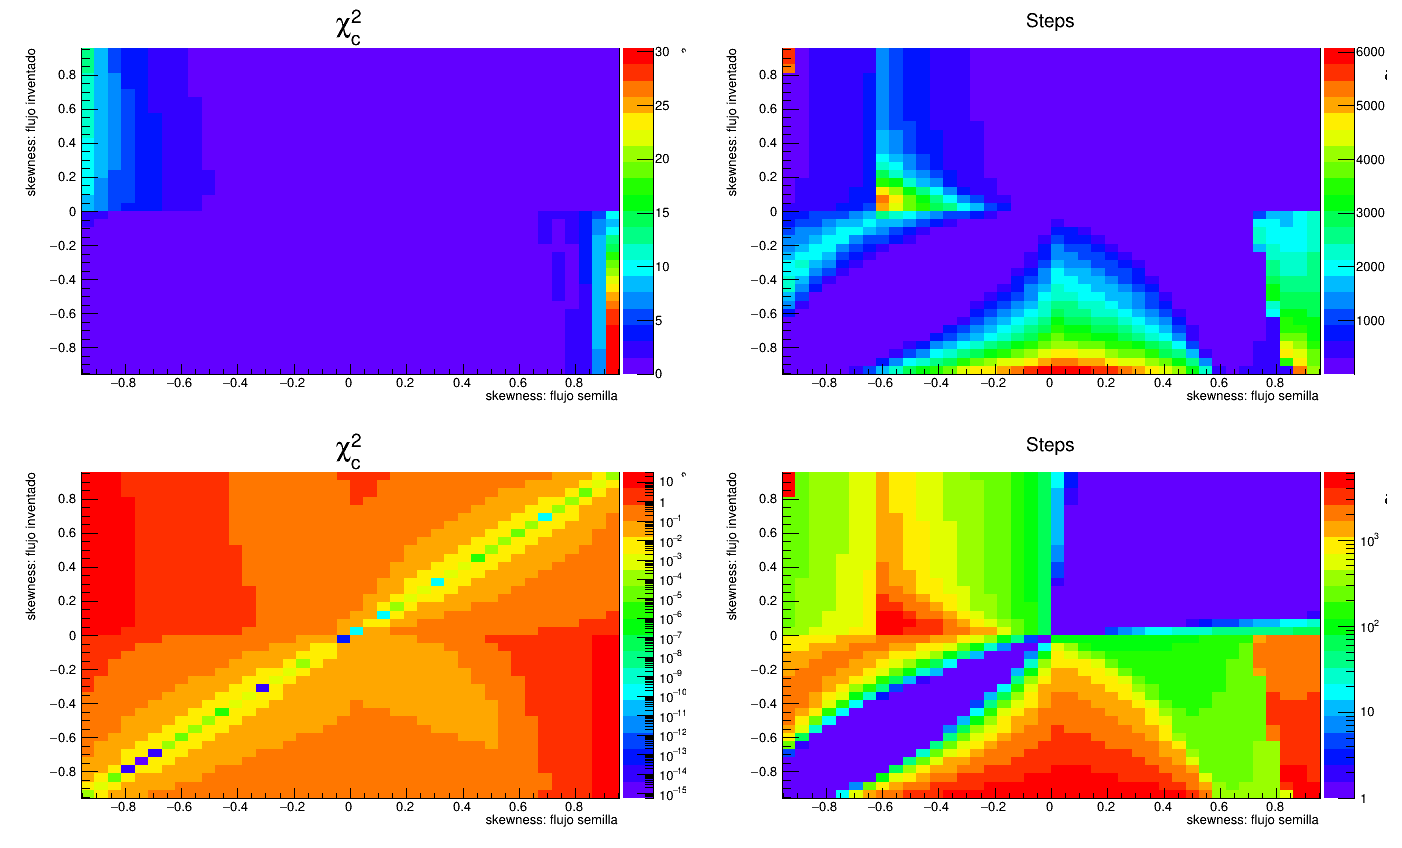
\includegraphics[width=1.\textwidth]{img/plot_deconv_33_tgraph_1.png}
    \centering
     \cprotect\caption{Grafico salida de la función \verb|neutrones_deconv_plot_33_tgraph()|. En los pad11 y 21 se grafica $\chi_c^2$ en función del valor del skewness del flujo semilla y el valor del skewness del flujo inventado.  En los pad12 y 22 se grafica los pasos que le toma converger a $\chi^2$  en función del valor del skewness del flujo semilla y el valor del skewness flujo inventado.} 
\label{plot_deconv_33_tgraph_skewness}
\end{figure}

 \begin{figure}[H]
    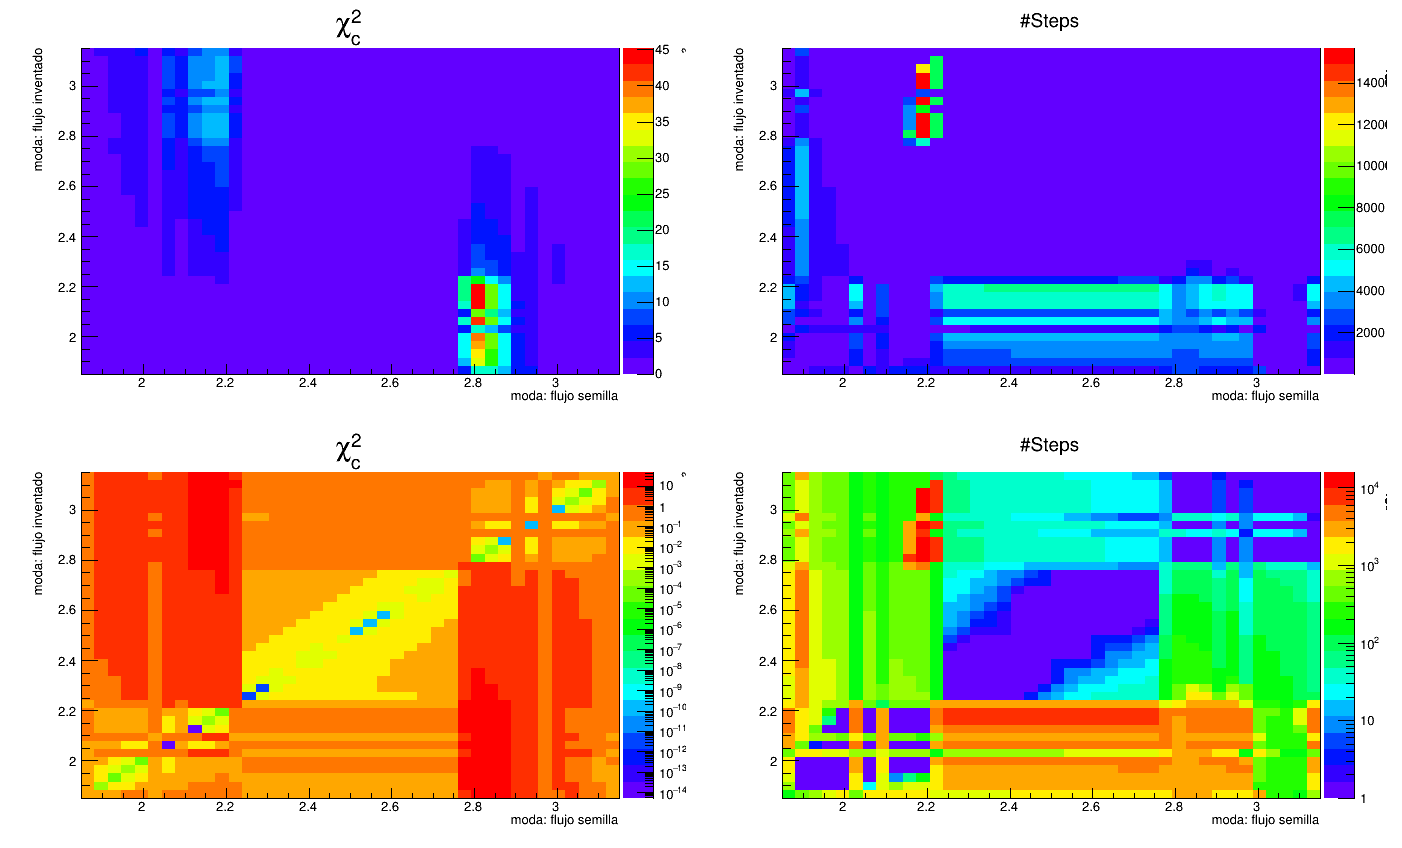
\includegraphics[width=1.\textwidth]{img/plot_deconv_33_tgraph_2.png}
    \centering
     \cprotect\caption{Grafico salida de la función \verb|neutrones_deconv_plot_33_tgraph()|. En los pad11 y 21 se grafica $\chi_c^2$ en función del valor de la moda del flujo semilla y el valor de $\gamma$ del flujo inventado.  En los pad12 y 22 se grafica los pasos que le toma converger a $\chi^2$  en función del valor de la moda del flujo semilla y el valor de $\gamma$ del flujo inventado.} 
\label{plot_deconv_33_tgraph_moda}
\end{figure}


Antes de continuar, revisando el código, se encontró en la línea 1883 de la clase \verb|ANPulses.cc| de la última actualización del repositorio en gitlab, en específico en la función \verb|Pretty_EMsimple_em1()|, una doble definición de \verb|chi2_em2|:

\begin{lstlisting}[language=c++]
	 chi2_em2 =  Xi_Square_em2(vec_fluxinv, vec_fluxdeconv,flux_inv->Integral() , flux_inv->GetNbinsX());chi2_em2 =  Xi_Square_em2(vec_fluxinv, vec_fluxdeconv,flux_deconv->Integral() , flux_inv->GetNbinsX());
\end{lstlisting}

En  principio la única repercusión que debería tener es en el tiempo de ejecución del código, ya que hace un cálculo repetido e innecesario. Por lo tanto, en la actualización siguiente del repositorio se elimina la definición repetida.

\subsection*{Entrada del 2022-01-14}

De la Fig. \ref{plot_deconv_33_tgraph_skewness} podemos ver en el pad21 que los menores valores de $\chi_c^2$ corresponden a la diagonal, esto es así ya que el método de la maximización de la expectación obtiene un mejor resultado de flujo deconvolucionado cuando la semilla es muy parecida al flujo inventado.

\subsection*{Reunión con los profesores Francisco Molina y Víctor Múñoz. (5ta)} 

Se muestran los resultados obtenidos de las simulaciones 31 (Fig. \ref{plot_deconv_31_tgraph_skewness}) y 33 (Fig. \ref{plot_deconv_31_tgraph_skewness}). Se comenta la extraña discontinuidad que se ve en el pad 21 de la Fig. \ref{plot_deconv_31_tgraph_skewness}, una de las posibles causas de esta es que al definir un valor de shape $\alpha$ para cada flujo semilla ( y por lo tanto un valor de skewness $\gamma$ asociado) se está moviendo al mismo tiempo tanto el centroide de la distribución (la moda para una distribución skew normal) como la amplitud de la distribución semilla (ver Fig. \ref{skew_normal_histogram_test_2}). Es decir, estamos observando el efecto en el algoritmo EM para el flujo deconvolucionado con respecto de la variación de dos valores, cuando en principio queremos estudiar el efecto de una sola variación, que es la deformación o skewness de la distribución semilla.

El profesor VM sugiere utilizar la nomenclatura de \textit{momentos} para referirnos a las propiedades de una distribución, como lo son: la media, varianza y skewness. También se sugiere seguir explorando en aplicar algoritmos de redes neuronales para obtener el flujo de neutrones medido por los detectores.

%----------------------------------------------------------------------------------------
%   REFERENCE LIST
%----------------------------------------------------------------------------------------
\clearpage
\appendix
\section{Resources}
\begin{tip}
It is a good idea to record sources that explain concepts or provide tools so the research is both better documented and if someone has to continue with it, there is enough supporting documentation.
\end{tip}
\begin{itemize}
    \item Quick read in DTW and Keogh Lower Bounding

\url{http://alexminnaar.com/time-series-classification-and-clustering-with-python.html}

\url{http://nbviewer.jupyter.org/github/alexminnaar/time-series-classification-and-clustering/blob/master/Time%20Series%20Classification%20and%20Clustering.ipynb}
    \item Parallelizing DTW -- Good article on making a parallel version of DTW. Uses Keogh lower bound not as a linear approximation but as a pruning device.

    \url{https://www.andrew.cmu.edu/user/mmohta/15418Project/finalreport.html}

    \item Deep Learning
    \begin{itemize}
        \item Intro to LSTM

        \url{https://colah.github.io/posts/2015-08-Understanding-LSTMs}
        
        \item Intro to CNN

        \url{https://colah.github.io/posts/2014-07-Conv-Nets-Modular/}

        \item Why are LSTMs are so useful, impressive result in character pattern and syntax learning

        \url{https://karpathy.github.io/2015/05/21/rnn-effectiveness/}
    \end{itemize}
\end{itemize}
\section{References}
\begin{tip}
Do not forget to cite the papers that you are using in your research, this way the \textbf{Previous Work} part in your paper will be infinitely easier to write when the time comes.
\end{tip}
\nocite{*}
\bibliographystyle{alpha}
\bibliography{mybib}
\clearpage
\section{TO DO}
\begin{tip}
Here you will have all your TODOs grouped with anchor links to the parts of the document where they are. Really handy if you do not know where to continue with your project.
\end{tip}
\listoftodos

\newpage

\section{Conceptos}


\begin{multicols}{2}
\subsection{Sistemas de adquisión de datos (DAQ)}

\begin{enumerate}
\item \textbf{Dead time}: Para un sistema de detección, es el tiempo mínimo de separación de dos eventos para que sean medidos como dos pulsos independientes. En algunos casos las limitaciones para este tiempo mínimo está determinada por los procesos en el detector mismo y en otros casos este límite está asociado a la electrónica del sistema de detección.

\item \textbf{Gain}

\item \textbf{Rango dinámico (de una señal)}

\item \textbf{Sampleo} La tarjeta digitalizadora samplea a 62.5 MHz (max 125 MHz), lo cual sirve para guardar el EFIR, obteniendo así una buena resolución en el espectro de altura de pulso, pero para guardar samples (pulsos) al samplear con esta frecuencia estaríamos sobre sampleando la señal, lo cuál se traduce en una mayor información digitalizada por sample, es decir, a un mayor tamaño del archivo .dlt. Es por esta razón, que para el experimento de neutrones pulsados se utilizó un clock externo que sampleaba la señal a 25 MHz.

\item \textbf{Ancho de ventana de adquisición de samples} Para la tarjeta digitalizadora Struck SIS3316-125-16, se tiene que cada bin corresponde a un ancho de tiempo de 40 ns, de esta manera, para un signal length (en GASIFIC) de $2^{16}-1=65535$ se tiene que la máxima ventana posible de adquisición de una señal (sample, para disparos) corresponde a $40 \phantom{!} \text{ns} \times 2^{16}-1  \approx 2.6 \phantom{!} \text{ms} $. Luego para movies (samples de neutrones de fondo) no necesitamos una ventana tan ancha de adquisición, ya que nos importa más la subida (para hacer el análisis de rise time usando TDC), de esta manera, para un signal length de $5000$ en GASIFIC, tenemos que la ventana de adquisición corresponde a $40 \phantom{!} \text{ns} \times 5000  \approx 0.2 \phantom{!} \text{ms} \phantom{@} (200 \mu s) $, la cuál es suficiente para capturar la forma de la subida de la señal.
\end{enumerate}


\subsection{Física Nuclear}

\begin{enumerate}

\item \textbf{Material Fisible}: $^{235}$U

\item \textbf{Material Fisionable} $^{238}$U

\item \textbf{Eficiencia Intrínseca de detección ($\varepsilon_{int}$)}: Corresponde a la probabilidad de detectar una partícula en un detector. No depende de la distancia a la fuente. 

\item \textbf{Eficiencia Absoluta de detección ($\varepsilon_{abs}$)}: Corresponde a la probabilidad de detectar una partícula emitida desde la fuente. Depende de la distancia fuente-detector.\\
\begin{align}
\varepsilon_{abs}=\varepsilon_{int} \frac{\Omega}{4\pi}
\end{align}

\item \textbf{Neutron Recoil}

\item \textbf{Flujo diferencial:}

\cprotEnv \begin{align}
\frac{d\Phi}{dE} \longrightarrow \verb|Flux[i]| =  \verb|Seed[i]| /\verb|dE[i]| 
\end{align}

\item \textbf{ Flujo integral:}

\cprotEnv \begin{align}
\frac{d\Phi}{dE}\cdot{dE} \rightarrow \verb|Flux[i]|= (\verb|Seed[i] |/\verb|dE[i]|) \verb|*dE[i]|
\end{align}

\subsection{Física de Plasmas}

\item \textbf{Drive parameter}: Este parámetro se define como:
\begin{align}
{\displaystyle {\frac {I}{a{\sqrt {\rho}}}}}
\end{align}
donde ${\displaystyle I}$ es la corriente, ${\displaystyle a}$ es el radio del ánodo, y ${\displaystyle \rho}$ es la densidad de gas o presión.\\
Es proporcional a la velocidad del plasma tanto en su fase axial como radial. Es uno de los parámetros más importantes que determina el rendimiento de un
PF como fuente de neutrones de fusión. Su valor constante en una amplia gama de PF's indica realmente que todos estos dispositivos funcionan a las mismas velocidades axial y radial y, por lo tanto, por inferencia, todos tienen las mismas temperaturas en las fases axial y radial \cite{Zhang2006} .
\item \textbf{Pinch lifetime ($t_{pf}$)}: Definido como el tiempo desde la primera compresión a un radio mínimo hasta el momento de la ruptura violenta de la columna de plasma. Con valores entre decenas de ns a 100-200 ns \cite{SingLee1996}. De acuerdo a CP, el $t_{pf}$ del PF400J es de 3 a 4 ns.
\subsection{Estadística}
\item \textbf{Skewness}: Es el tercer momento estándar de una distribución de probabilidad y da cuenta de la asimetría de esta. El grado de asimetría de una distribución se denomina sesgo hacia la derecho o hacia la izquierda




\end{enumerate}

\end{multicols}

\end{document}